% !TeX program = xelatex
% !TeX encoding = UTF-8
\documentclass{MathorCupmodeling}
\usepackage{mwe,color,float}
\usepackage[linesnumbered,ruled]{algorithm2e}
\usepackage{setspace}
\usepackage{pdfpages}
\extrafloats{100}
\bianhao{MCB2201112}
\tihao{B}
\timu{\textbf{基于多模型调参优化的Stacking用户评分预测集成学习}}
\keyword{特征工程;合理性分析;Stacking集成学习;评分预测;可视化评估}
\begin{document}
	\begin{abstract}
		随着移动通信技术的迅猛发展和网络工程的不断建设,在信息透明、产品同质化的今天,提升语音通话及网络服务的质量,满足用户对高质量语音通话、网络服务的需求显得尤为重要。本文旨在\textbf{建立一个基于多模型调参优化的Stacking集成学习},\textbf{完善且合理地预测用户评分的普适性模型},从已有数据中心获得有效信息,更高效地提升服务质量,从而完善业务服务体系。

		{\heiti 针对问题一},本文分析了语音及上网业务用户评分高分与低分的特征,并对用户评分的合理性进行分析。在此基础上筛选出评分较为合理的用户数据,利用该数据建立预测模型,对用户评分进行预测,并解释合理性。本文首先对数据集进行统一处理,包括:\textbf{初步剔除相关列数据}、\textbf{学习数据与预测数据指标一致化}、\textbf{指标规范化}、\textbf{空缺值处理}、\textbf{标签编码}、\textbf{特征构造}、\textbf{数据标准化}、\textbf{学习数据与预测数据一致化}、\textbf{学习数据训练集与测试集划分}。在此基础上,我们综合用户评分箱线图、皮尔逊相关系数热力图、联合分布图,在保证评分数据不失真的情况下,计算出用户对于某一业务的整体评分,并将评分划分为高分组、中间组、低分组。之后着重分析高分组与低分组用户特征,并进行比较,得到一般性结论,发现高分组与低分组用户差异较为明显,比如:无论是语音还是上网业务,高分组近半成用户手机品牌均为“华为”,而低分组超半成用户手机品牌均为“苹果”……同时,本文由此分析各用户评分的合理性,确定剔除不合理评分用户的标准及方案,以多元指标进行剔除,最终筛选出评分合理的用户群体,语音业务及上网业务数据保留率分别为97.88 \%,97.12 \%。在此基础上,本文重新建立与初赛一致的多种多分类预测模型,并依据模型准确率、平均绝对误差、均方误差等指标进行Stacking集成学习,预测结果符合预期效果,各评分预测模型效果见\textcolor{blue}{\cref{tab:StackingResult2}},明显优于单一模型。在保证准确率的同时,预测的平均绝对误差、均方误差\textbf{均有一定优化},同时本文还注重结果的可解释性及模型的现实意义。此外,本文绘制出模型的\textbf{混淆矩阵热力图}、\textbf{分类报告}、\textbf{ROC/AUC曲线},多方面评估模型效果及解释模型的合理性。此外,我们还将初赛中模型与复赛中模型进行对比,发现模型的平均绝对误差及均方误差均大幅度提升,详见\textcolor{blue}{\cref{tab:优化结果}},其中平均绝对误差最高提升12.47 \%,均方误差最高提升18.06 \%;此外本文还对比模型可视化效果,发现模型各项指标均优于初赛中模型,效果良好。
		
		{\heiti 针对问题二},我们结合初赛及复赛问题一的分析、研究结果,设计出一份非技术性报告,将本文的发现提供给中国移动公司,并提出建设性、可执行性建议。
		
		{\heiti 最后},本文对所建立的模型的优缺点进行了中肯的评价、提出了模型的改进措施以及对模型进行了一定推广。
	\end{abstract}

	\pagestyle{empty}
	\tableofcontents
	\newpage
	\pagestyle{fancy}

	\setcounter{page}{1}
	\section{问题的提出}
	\subsection{问题背景}
	随着移动通信技术的迅猛发展和网络工程的不断建设,在信息透明、产品同质化的今天,提升语音通话及网络服务的质量,满足用户对高质量语音通话、网络服务的需求显得尤为重要。由于当今用户数量的不断增多、用户需求不断提高、运营商业务不断广泛化,因此点对点、传统方法解决问题逐渐困难化。而现在有来自移动通信集团北京分公司根据用户对语音业务及上网业务的满意度进行的评分及相关影响因素的数据,我们需要对其进行分析、建立相关数学模型,以便从数据中心获得有效信息,更高效地提升服务质量,为客户提供更好的服务。
	\subsection{问题要求}
	\begin{itemize}
		\item 初赛要求:
		\begin{itemize}
			\item \textbf{问题一}:研究并量化分析影响用户对语音及上网业务满意度的主要因素;
			\item \textbf{问题二}:建立基于影响用户评分影响因素的数学模型,并依据附件3、4中相关因素对其评分进行预测,并解释预测评分的合理性。
		\end{itemize}
		\item 复赛要求:
		\begin{itemize}
			\item \textbf{问题一}:结合初赛的分析、研究结果,分析用户对语音及上网业务的评分高低,并得出高分组与低分组的特征;同时对客户评分的合理性进行分析,筛选出评分合理的客户数据,并利用新的数据集重新建立预测模型,再对附件3、4中评分进行预测;
			\item \textbf{问题二}:依据初赛及复赛的分析结果,设计一份不超过一页纸的非技术报告,并将发现及建议提供给中国移动北京公司。
		\end{itemize}
	\end{itemize}

	\textbf{本文将在初赛的基础上完成复赛问题要求,且解决问题的大方向不变。同时大多解决方案与初赛一致,对于特定问题,我们也将进行合理地修改。}

	\section{问题的分析}
	\subsection{问题的整体分析}
	该题是一个关于移动用户对语音及上网业务体验评分的数据分析、预测类问题。

	\textbf{从分析目的看},本题需要结合初赛的分析、研究结果,对数据集进行再分析,分析评分高分组与低分组的各自特征,对原数据集进行重采样,进行更深层次的分析。同时需要对用户的评分进行预测及研究,为运营商提供参考,从而提升用户语音及上网的优质体验。因此本题主要需完成两方面任务:{\heiti 其一},结合初赛的分析、研究结果,分析用户对语音及上网业务的评分高低,并得出高分组与低分组的特征;同时对客户评分的合理性进行分析,筛选出评分合理的客户数据,并利用新的数据集重新建立预测模型,再对附件3、4中评分进行预测;{\heiti 其二},依据初赛及复赛的分析结果,设计一份不超过一页纸的非技术报告,并将发现及建议提供给中国移动北京公司。

	\textbf{从数据来源、特征看},本题的数据来源于北京移动用户的语音与上网业务评分数据,数据包括用户对语音业务下“语音通话整体满意度”“网络覆盖与信号强度”“语音通话清晰度”“语音通话稳定性”,上网业务下“手机上网整体满意度”“网络覆盖与信号强度”“手机上网速度”“手机上网稳定性”方面的评分,以及相关的影响评分的因素。评分数据具有主观性,影响因素数据具有高维、多样、标准体系不一致、量纲不一致等特点,且数据量较大。因此,本题数据相对特殊且复杂,需要对数据进行一定的预处理,以便于后续的分析。
	
	\textbf{从模型的选择看},本题数据量较大、维度较高,且分析目的是分析影响用户评分的主要因素,并对用户的评分进行预测及研究。本文将评分视为多分类,且评分具有一定主观性、分类种类多,因此,在模型的选择上,本文结合多种分类预测模型,构建集成学习模型,尽可能多地学习到用户评分特点,提升模型的准确性、稳健性及可泛化性能。

	\textbf{从软件的选择看},本题为数据类型,且需要进行大量的数据分析、预测等,因此我们选择Python Jupyter对问题进行求解,其交互式的编程范式,方便且高效。

	\subsection{初赛总结}
	{\heiti 针对问题一},主要需要对用户语音及上网业务评分影响因素的程度进行量化分析。我们首先对数据集进行统一处理,包括:\textbf{初步剔除相关列数据}、\textbf{学习数据与预测数据指标一致化}、\textbf{指标规范化}、\textbf{空缺值处理}、\textbf{标签编码}、\textbf{特征构造}、\textbf{数据标准化}、\textbf{学习数据与预测数据一致化}、\textbf{学习数据训练集与测试集划分}。之后在处理好的数据集上建立\textbf{熵权法}、\textbf{灰色关联度分析}、\textbf{随机森林分类}模型,多方面综合考虑,量化分析各影响因素对评分的影响程度,并依此来确定影响评分的主要因素。量化结果接近于实际生活,效果良好,且可为后续问题奠定基础。
	
	{\heiti 针对问题二},主要需要根据已有影响因素对用户的评分进行预测,并解释预测的合理性。我们首先结合问题一量化结果以及建立\textbf{主成分分析}模型,对数据\textbf{累计方差}进行解释,确定特征个数;之后建立\textbf{XGBoost模型},并得出各影响因素的重要性,与随机森林模型结合分析,确定特征的选择;再建立\textbf{KNN}、\textbf{SVM}、\textbf{LightGBM}以及\textbf{多分类逻辑回归模型},对数据进行学习分析;随后,对各个模型进行\textbf{超参数调优},模型准确率均有大幅度提升,如随机森林\textbf{较原先提升了}$\boldsymbol{11.69\%}$,\textbf{最高提升较原先可达到}$\boldsymbol{14.25\%}$,效果良好。再者,以模型的准确率、平均绝对误差、均方误差为标准,选择表现较优的模型作为\textbf{Stacking集成学习}的基模型,同时选择余下的一个模型作为第二层模型,在提升准确率的同时,避免过拟合。同时对其采用\textbf{五折交叉验证},验证其\textbf{稳健性}。Stacking集成学习结果符合预期效果,且明显优于单一模型。在保证准确率的同时,预测的平均绝对误差、均方误差\textbf{均有一定优化},同时我们还注重结果的可解释性及模型的现实意义。最后,我们进行\textbf{可视化分析},绘制原始数据及预测数据评分人数\textbf{南丁格尔玫瑰图},查看数据分布,绘制模型的\textbf{混淆矩阵热力图}、\textbf{分类报告}、\textbf{ROC/AUC曲线},多方面评估模型效果及解释模型的合理性。综合上述分析,可以确认模型效果良好,具有良好的稳健性、泛化能力。
	
	{\heiti 最后},我们还对所建立的模型的优缺点进行了中肯的评价、提出了模型的改进措施以及对模型进行了一定推广。

	\subsection{问题一的分析}
	问题一的核心目的在于\textbf{对原数据集进行重采样,并进行更深层次的分析}。对于主观性因素过强的用户评分数据,为尽可能提升预测的准确率,我们需要先筛选出高分组及低分组用户,对其行为特征进行分析,筛选出评分合理的用户,依此重新建立分类预测模型,提升移动公司对用户对各项业务的满意程度的把握程度,从而更好地解决现存问题,为用户提供更优质服务。
	\subsection{问题二的分析}
	问题二的核心目的在于\textbf{为移动公司撰写一份非技术性报告,为其提供合理性建议,从而为客户提供更好的服务}。
	\section{符号说明}
	\begin{center}
		\scalebox{0.92}{
		\begin{tabularx}{0.7\textwidth}{c@{\hspace{1pc}}|@{\hspace{2pc}}X}
			\Xhline{0.08em}
			符号 & \multicolumn{1}{c}{符号说明}\\
			\Xhline{0.05em}
			$\mu$ & 样本平均值\\
			$\sigma$ & 样本方差\\
			$x_{\mathrm{standard}}$ & 经过标准化后的数据\\
			$R\left(x\right)_{m\times n}$ & 经过某项处理后的数据特征集\\
			$\rho$ & 皮尔逊相关系数\\
			$x'$ & 经过某项处理后的数据\\
			$Gini$ & 样本集合基尼系数\\
			$\hat{y}$ & 预测值\\
			$L^{\left(t\right)}$ & 目标函数\\
			$\Omega$ & 叶节点正则项惩罚系数\\
			$P$ & 某事件发生的概率\\
			$\omega$ & 权重\\
			\Xhline{0.08em}
		\end{tabularx}}
	\end{center}
	\section{模型的假设}
	本文对于模型的假设与初赛假设一致,如下:
	\begin{itemize}
		\item \textbf{假设一}:语音与上网业务的八项评分中,存在个别用户乱评、错评现象;
		\item \textbf{假设二}:除个别用户的部分评分外,其余所有数据真实且符合实际情况;
		\item \textbf{假设三}:用户评分还受到除附件中因素之外的因素的影响;
		\item \textbf{假设四}:给定的数据集可全面体现用户整体情况;
		\item \textbf{假设五}:对于同一业务,学习数据与预测数据的内在规律是一致的。
	\end{itemize}
	\section{模型的建立与求解}
	\subsection{相关准备工作}
	为方便、准确、高效解决问题,我们需要对数据进行预处理,处理过程与初赛大致相同,但本文对部分操作进行的合理地修改,以适应本题要求。主要过程见\textcolor{blue}{\cref{fig:dataprepare}},包括:初步剔除相关列数据、学习数据与预测数据指标一致化、指标规范化、空缺值处理、标签编码、特征构造、标准化、学习数据与预测数据一致化、学习数据训练集与测试集划分。\textbf{本文后续的模型建立都在此基础之上}。
	\begin{figure}[H]
		\centerline{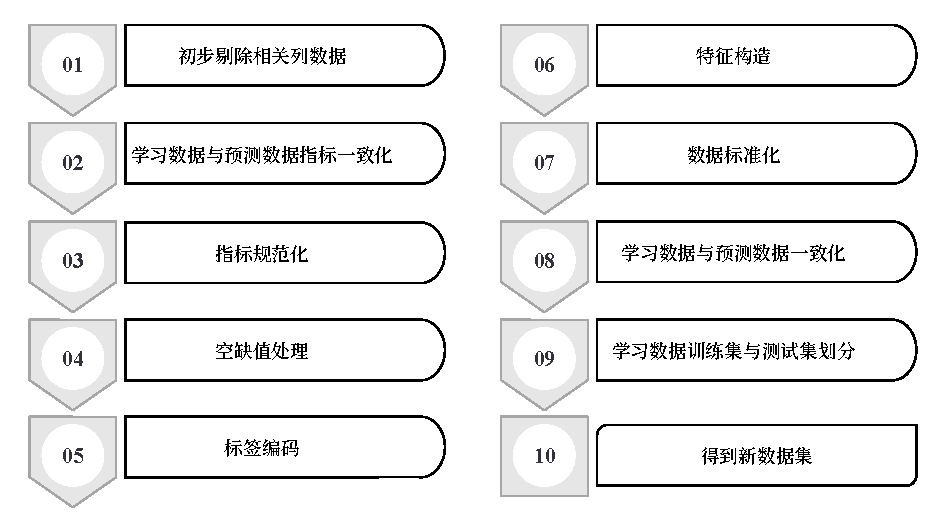
\includegraphics[scale=0.78]{数据的准备.pdf}}
		\caption{数据的准备主要过程}\label{fig:dataprepare}
	\end{figure}
	\begin{itemize}
		\item \textbf{Step1 初步剔除相关列数据}
		
		由于“用户id”为连续编号,且与评分无任何关系,故本文将该列数据剔除;同时对于“用户描述”等文字性叙述指标,由于其均为文本,且描述特征难以提取,难以量化,本文将该列数据剔除,但为了获得客户相关描述,本文将绘制用户描述高频词汇云图;此外,对于“终端品牌类型”等多类别指标,由于其类别较多,量化后难以提取出有效信息,故也将其剔除,其余列暂时保留。

		\item \textbf{Step2 学习数据与预测数据指标一致化}
		
		附件1与附件3为用户语音业务数据,但两表数据影响的因素存在不一致的现象,需要对指标取交集,确保两者一致,附件2与附件4同理。这里我们利用Python中集合set容器元素唯一性特征及pandas库,筛选出相同因素。而对于可能重合的指标,我们在下文也会进行一定处理。这样即可确保在学习数据上建立的模型依据的指标存在于预测数据集上,避免两者指标不一的情况。

		\item \textbf{Step3 指标规范化}
		
		经过上述处理后,我们发现大部分影响因素为分类指标,其划分“是”“否”的字段不统一,故依据“附件5附件1、2、3、4的字段说明.xlsx”文件,本文对附件1、2、3、4中的分类指标进行规范化,记“是”类别为1,“否”类别为0,方便后续模型的建立。

		\item \textbf{Step4 空缺值处理}
		
		在给定数据集中,部分空缺值可以依据附件5的解释进行填充。经过一定处理后,附件3与附件4中无空缺值,故本文对附件1与附件2中的空缺值进行分析与处理:
		\begin{itemize}
			\item \textbf{对于附件1}:据附件5解释进行填充后,还存在个别用户的空缺值,空缺值的列名为:“是否4G网络客户(本地剔除物联网)”“终端品牌”“是否5G网络客户”“客户星级标识”,且这些空缺值均在同一用户中出现,用户id分别为1573、1601、2326、2827、3265。附件1的空缺值有集中、个数少的特点,存有空缺值的用户仅有5个,占整体用户的$0.0920\%$,对于模型的建立影响较小,因此我们将这5行用户剔除。
			\item \textbf{对于附件2}:经过指标一致化后及初步数据空缺值的填补后,附件2中仅剩“终端品牌”列指标存在14个空缺值,根据该列数据其余特征,我们将这个14个空缺值以0填充。
		\end{itemize}

		\item \textbf{Step5 标签编码}
		
		首先,对用户的评分进行编码,由于部分分类模型需要分类量值从0开始,因此,为方便后续集成学习等,本文将评分从$\left[1,10\right]$映射至$\left[0,9\right]$,且仍均为整数,即将评分减1。其次,对“终端品牌”“4\textbackslash{}5G用户”指标利用Python的sklearn库中的LabelEncoder进行标签编码。此外,对于“客户星级标识”指标,我们依据移动公司对客户星级标识的划分进行编码,编码值对应见\textcolor{blue}{\cref{tab:客户星级标志对应表}}。
		\begin{table}[htbp]
			\centering
			\caption{客户星级标识编码对应表}\label{tab:客户星级标志对应表}
			\scalebox{0.8}{
			\begin{tabular}{ccccccccc}
				\toprule
				未评级 & 准星 & 一星 & 二星 & 三星 & 银卡 & 金卡 & 白金卡 & 钻石卡 \\
				\midrule
				0 & 1 & 2 & 3 & 4 & 5 & 6 & 7 & 8 \\
				\bottomrule
			 \end{tabular}}
		\end{table}

		\item \textbf{Step6 特征构造}
		
		观察并分析给定的数据,我们可以构造以下特征:
		\begin{itemize}
			\item \textbf{对于附件1与附件3}:
			\begin{itemize}
				\item 观察到附件1中有“家宽投诉”与“资费投诉”两项,而在附件3中有“是否投诉”一项,因此,我们在附件1中构造“是否投诉”一项。若“家宽投诉”与“资费投诉”均为0,则“是否投诉”记为0,否则记为1。并同时删去“家宽投诉”与“资费投诉”;
				\item 观察到附件1中有多个出现问题的场所,因此我们将每一用户出现问题的场所求和,构造“场所合计”,他们为“居民小区”“办公室”“高校”“商业街”“地铁”“农村”“高铁”“其他,请注明”;
				\item 观察到附件1中有多个类型的问题,因此我们将出现问题求和,构造出“出现问题合计”,他们为“手机没有信号”有信号无法拨通”“通话过程中突然中断”“通话中有杂音、听不清、断断续续”“串线”“通话过程中一方听不见”“其他,请注明.1”;
				\item 观察到附件1中“脱网次数”“mos质差次数”“未接通掉话次数”有相似特征,故将每一用户该三项数据求和,构造出“脱网次数、mos质差次数、未接通掉话次数合计”。
			\end{itemize}
			\item \textbf{对于附件2与附件4}:
			\begin{itemize}
				\item 观察到附件2中有多个出现问题的场所,构造出“出现问题场所或应用总”;
				\item 观察到附件2中“手机上网速度慢”“打游戏延时大”“显示有信号上不了网”“全部都卡顿”“全部游戏都卡顿”“手机支付较慢”“看视频卡顿”“上网过程中网络时断时续或时快时慢”“打开网页或APP图片慢”“全部网页或APP都慢”“下载速度慢”“网络信号差/没有信号”特征相似,故将每一用户对应的项目数据求和,构造出”网络卡速度慢延时大上不了网总“;
				\item 观察到附件2中“微信质差次数”以及“上网质差次数”均为质差量值,故将每一用户该二项数据求和,构造出“质差总”;
				\item 观察到附件2中的场所类别较多,故将场所求和,构造出“地点总”。
			\end{itemize}
		\end{itemize}

		\item \textbf{Step7 数据标准化}
		
		该处标准化处理为\textbf{Z-score}方法,仅用于后续机器学习模型的使用。而在问题一的熵权法、灰色关联度分析中我们采用\textbf{Min-Max}方法,该方法在后文模型中会具体说明。

		对于某一列数据$x=\left[x_1,x_2,\cdots,x_m\right]^{\mathrm{T}}$,其平均值为
		\begin{equation}
			\mu=\frac{1}{m}\sum_{i=1}^{m}x_i \label{fmean}
		\end{equation}
		标准差为
		\begin{equation}
			\sigma=\sqrt{\frac{1}{m}\sum_{i=1}^{m}\left(x_i-\mu\right)^2} \label{fstd}
		\end{equation}
		则标准化后的数据为
		\begin{equation}
		\left(x_{\mathrm{standard}}\right)_i=\frac{x_i-\mu}{\sigma} \label{fstandardprocess}
		\end{equation}

		利用上述计算公式,我们对非分类指标进行处理,使得原数据经过处理后,其值聚集于0附近,即均值为0,标准差为1。这样处理,利于机器学习模型的建立、学习与预测,加快模型的收敛速度,并在一定程度上提升模型的准确性。同时该标准化处理方法适合当代嘈杂的大数据场景\textcolor{blue}{\cite{pstandard}}。因此对于大样本的数据,如出现部分异常值,使用该方法对最终结果影响较小。

		\item \textbf{Step8 学习数据与预测数据一致化}
		
		经过上述几项处理后,我们还需要将附件1与附件3数据集一致化,包括指标一致化以及数据字段、分布排列一致化,从而保证对于需要预测的数据集附件3利用在附件1中建立的模型所利用到的数据集的一致性,避免造成数据的不一致,导致预测错误。本文对附件2与附件4进行上述相同的操作。

		\item \textbf{Step9 学习数据训练集与测试集划分}
		
		为计算问题二中建立的模型的准确性等指标,需要在附件1与附件2中均划分训练集与测试集。对于语音业务划分训练集与测试集比例为8:2;而对于上网业务,其比例设为9:1。对于比例的设置,本文将在后文解释其合理性。且上述划分利用sklearn库中的train\_test\_split函数实现,且任意设定随机种子为2022,确保多次调试结果的一致性。该函数可确保划分的随机性,确保训练集与测试集数据分布规律大致相同。

	\end{itemize}
	
	\subsection{初赛研究相关结论}
	在初赛中,我们通过熵权法、灰色关联度分析以及随机森林多分类模型,量化影响用户评分的各因素,并得出主要因素,结果见\textcolor{blue}{\cref{tab:语音业务影响因素量化}},\textcolor{blue}{\cref{tab:上网业务影响因素量化1}}及\textcolor{blue}{\cref{tab:上网业务影响因素量化2}}。
	\begin{table}[htbp]
		\centering
		\caption{语音业务总体以及四项评分各个指标影响程度量化结果}
		\setlength{\aboverulesep}{0pt}
		\setlength{\belowrulesep}{0pt}
		\scalebox{0.66}{
		  \begin{tabular}{c|cccc|c}
		  \toprule
		  \textbf{因素} & \textbf{语音通话整体满意度} & \textbf{网络覆盖与信号强度} & \textbf{语音通话清晰度} & \textbf{语音通话稳定性} & \textbf{语音业务总} \\
		  \midrule
		  GPRS总流量(KB) & 0.1266  & 0.1151  & 0.1181  & 0.1263  & 0.1215  \\
		  当月ARPU & 0.1154  & 0.1116  & 0.1000  & 0.1032  & 0.1111  \\
		  是否遇到过网络问题 & 0.0922  & 0.1015  & 0.0953  & 0.1080  & 0.0995  \\
		  前3月MOU & 0.0996  & 0.1232  & 0.1028  & 0.0993  & 0.0964  \\
		  语音通话-时长(分钟) & 0.0726  & 0.0762  & 0.0754  & 0.0680  & 0.0747  \\
		  当月MOU & 0.0671  & 0.0715  & 0.0722  & 0.0689  & 0.0673  \\
		  mos质差次数 & 0.0645  & 0.0512  & 0.0617  & 0.0670  & 0.0604  \\
		  脱网次数  & 0.0388  & 0.0406  & 0.0361  & 0.0444  & 0.0372  \\
		  未接通掉话次数 & 0.0334  & 0.0319  & 0.0328  & 0.0302  & 0.0327  \\
		  客户星级标识 & 0.0315  & 0.0233  & 0.0259  & 0.0243  & 0.0316  \\
		  终端品牌  & 0.0356  & 0.0297  & 0.0368  & 0.0382  & 0.0310  \\
		  4\textbackslash{}5G用户 & 0.0114  & 0.0137  & 0.0177  & 0.0119  & 0.0212  \\
		  GPRS-国内漫游-流量(KB) & 0.0105  & 0.0112  & 0.0162  & 0.0136  & 0.0145  \\
		  高铁    & 0.0107  & 0.0114  & 0.0141  & 0.0118  & 0.0124  \\
		  农村    & 0.0117  & 0.0106  & 0.0105  & 0.0076  & 0.0124  \\
		  地铁    & 0.0151  & 0.0126  & 0.0152  & 0.0129  & 0.0121  \\
		  通话过程中突然中断 & 0.0081  & 0.0134  & 0.0096  & 0.0075  & 0.0117  \\
		  外省流量占比 & 0.0133  & 0.0125  & 0.0110  & 0.0094  & 0.0115  \\
		  是否5G网络客户 & 0.0116  & 0.0090  & 0.0128  & 0.0091  & 0.0112  \\
		  商业街   & 0.0096  & 0.0080  & 0.0124  & 0.0071  & 0.0109  \\
		  手机没有信号 & 0.0167  & 0.0076  & 0.0142  & 0.0177  & 0.0108  \\
		  套外流量费(元) & 0.0063  & 0.0077  & 0.0089  & 0.0102  & 0.0106  \\
		  通话过程中一方听不见 & 0.0112  & 0.0121  & 0.0171  & 0.0085  & 0.0093  \\
		  外省语音占比 & 0.0023  & 0.0069  & 0.0051  & 0.0066  & 0.0091  \\
		  居民小区  & 0.0115  & 0.0112  & 0.0091  & 0.0148  & 0.0086  \\
		  办公室   & 0.0073  & 0.0145  & 0.0117  & 0.0085  & 0.0085  \\
		  省际漫游-时长(分钟) & 0.0086  & 0.0114  & 0.0078  & 0.0060  & 0.0081  \\
		  串线    & 0.0053  & 0.0036  & 0.0035  & 0.0057  & 0.0079  \\
		  套外流量(MB) & 0.0071  & 0.0070  & 0.0037  & 0.0070  & 0.0071  \\
		  通话中有杂音、听不清、断断续续 & 0.0105  & 0.0078  & 0.0067  & 0.0106  & 0.0070  \\
		  其他,请注明 & 0.0040  & 0.0052  & 0.0050  & 0.0065  & 0.0058  \\
		  有信号无法拨通 & 0.0076  & 0.0051  & 0.0087  & 0.0088  & 0.0058  \\
		  其他,请注明.1 & 0.0036  & 0.0065  & 0.0040  & 0.0048  & 0.0051  \\
		  是否关怀用户 & 0.0070  & 0.0041  & 0.0055  & 0.0059  & 0.0044  \\
		  是否投诉  & 0.0028  & 0.0029  & 0.0047  & 0.0032  & 0.0041  \\
		  高校    & 0.0039  & 0.0038  & 0.0049  & 0.0033  & 0.0031  \\
		  前3月ARPU & 0.0044  & 0.0037  & 0.0022  & 0.0030  & 0.0031  \\
		  是否4G网络客户(本地剔除物联网) & 0.0008  & 0.0005  & 0.0009  & 0.0004  & 0.0005  \\
		  \bottomrule
		  \end{tabular}}
		\label{tab:语音业务影响因素量化}
	\end{table}
	\begin{table}[htbp]
		\centering
		\caption{上网业务总体以及四项评分各个指标影响程度量化结果[续表见\textcolor{blue}{\cref{tab:上网业务影响因素量化2}}]}
		\setlength{\aboverulesep}{0pt}
		\setlength{\belowrulesep}{0pt}
		\scalebox{0.66}{ 
		  \begin{tabular}{c|cccc|c}
		  \toprule
		  \textbf{因素} & \textbf{手机上网整体满意度} & \textbf{网络覆盖与信号强度} & \textbf{手机上网速度} & \textbf{手机上网稳定性} & \textbf{上网业务总} \\
		  \midrule
		  当月MOU & 0.1563  & 0.2447  & 0.2530  & 0.2436  & 0.2278  \\
		  网络卡速度慢延时大上不了网总 & 0.0899  & 0.1259  & 0.0292  & 0.1295  & 0.1244  \\
		  终端品牌  & 0.0332  & 0.0484  & 0.0643  & 0.0594  & 0.0551  \\
		  客户星级标识 & 0.0223  & 0.0596  & 0.0531  & 0.0549  & 0.0522  \\
		  出现问题场所或应用总 & 0.4678  & 0.0402  & 0.1258  & 0.0407  & 0.0394  \\
		  性别    & 0.0242  & 0.0440  & 0.0286  & 0.0315  & 0.0387  \\
		  脱网次数  & 0.0383  & 0.0282  & 0.0284  & 0.0323  & 0.0318  \\
		  质差总   & 0.0107  & 0.0289  & 0.0334  & 0.0330  & 0.0317  \\
		  是否5G网络客户 & 0.0092  & 0.0301  & 0.0350  & 0.0267  & 0.0296  \\
		  微信质差次数 & 0.0104  & 0.0251  & 0.0205  & 0.0210  & 0.0233  \\
		  是否不限量套餐到达用户 & 0.0078  & 0.0183  & 0.0189  & 0.0172  & 0.0226  \\
		  套外流量费(元) & 0.0089  & 0.0206  & 0.0249  & 0.0213  & 0.0221  \\
		  上网质差次数 & 0.0058  & 0.0185  & 0.0208  & 0.0183  & 0.0215  \\
		  农村    & 0.0067  & 0.0154  & 0.0150  & 0.0154  & 0.0163  \\
		  显示有信号上不了网 & 0.0105  & 0.0131  & 0.0146  & 0.0150  & 0.0161  \\
		  居民小区  & 0.0138  & 0.0185  & 0.0185  & 0.0170  & 0.0161  \\
		  地铁    & 0.0100  & 0.0141  & 0.0145  & 0.0169  & 0.0151  \\
		  高铁    & 0.0016  & 0.0138  & 0.0123  & 0.0123  & 0.0150  \\
		  商业街   & 0.0090  & 0.0124  & 0.0127  & 0.0149  & 0.0139  \\
		  上网过程中网络时断时续或时快时慢 & 0.0038  & 0.0102  & 0.0107  & 0.0103  & 0.0137  \\
		  网络信号差/没有信号 & 0.0046  & 0.0109  & 0.0138  & 0.0139  & 0.0133  \\
		  办公室   & 0.0091  & 0.0136  & 0.0156  & 0.0144  & 0.0120  \\
		  套外流量(MB) & 0.0029  & 0.0107  & 0.0089  & 0.0134  & 0.0119  \\
		  手机支付较慢 & 0.0000  & 0.0073  & 0.0069  & 0.0058  & 0.0086  \\
		  其他,请注明 & 0.0031  & 0.0123  & 0.0090  & 0.0100  & 0.0079  \\
		  下载速度慢 & 0.0023  & 0.0073  & 0.0071  & 0.0067  & 0.0074  \\
		  拼多多   & 0.0000  & 0.0035  & 0.0033  & 0.0038  & 0.0063  \\
		  打游戏延时大 & 0.0094  & 0.0044  & 0.0033  & 0.0025  & 0.0063  \\
		  抖音    & 0.0015  & 0.0081  & 0.0072  & 0.0051  & 0.0059  \\
		  百度    & 0.0000  & 0.0064  & 0.0048  & 0.0061  & 0.0059  \\
		  其他,请注明.1 & 0.0033  & 0.0041  & 0.0028  & 0.0056  & 0.0059  \\
		  看视频卡顿 & 0.0020  & 0.0056  & 0.0054  & 0.0055  & 0.0056  \\
		  微信    & 0.0012  & 0.0054  & 0.0042  & 0.0051  & 0.0052  \\
		  \bottomrule
		  \end{tabular}}
		\label{tab:上网业务影响因素量化1}
	\end{table}
	\begin{table}[htbp]
		\centering
		\caption{上网业务总体以及四项评分各个指标影响程度量化结果[\textcolor{blue}{\cref{tab:上网业务影响因素量化1}}续表]}
		\setlength{\aboverulesep}{0pt}
		\setlength{\belowrulesep}{0pt}
		\scalebox{0.66}{
		  \begin{tabular}{c|cccc|c}
		  \toprule
		  \textbf{因素} & \textbf{手机上网整体满意度} & \textbf{网络覆盖与信号强度} & \textbf{手机上网速度} & \textbf{手机上网稳定性} & \textbf{上网业务总} \\
		  \midrule
		  高校    & 0.0000  & 0.0046  & 0.0063  & 0.0052  & 0.0051  \\
		  腾讯视频  & 0.0022  & 0.0042  & 0.0044  & 0.0040  & 0.0049  \\
		  打开网页或APP图片慢 & 0.0054  & 0.0042  & 0.0045  & 0.0042  & 0.0044  \\
		  全部网页或APP都慢 & 0.0023  & 0.0031  & 0.0030  & 0.0028  & 0.0044  \\
		  京东    & 0.0000  & 0.0064  & 0.0041  & 0.0060  & 0.0043  \\
		  快手    & 0.0000  & 0.0026  & 0.0058  & 0.0042  & 0.0041  \\
		  淘宝    & 0.0022  & 0.0044  & 0.0043  & 0.0054  & 0.0040  \\
		  手机上网速度慢 & 0.0022  & 0.0031  & 0.0032  & 0.0034  & 0.0038  \\
		  今日头条  & 0.0000  & 0.0047  & 0.0044  & 0.0048  & 0.0035  \\
		  王者荣耀  & 0.0000  & 0.0030  & 0.0021  & 0.0020  & 0.0034  \\
		  新浪微博  & 0.0000  & 0.0039  & 0.0033  & 0.0041  & 0.0029  \\
		  爱奇艺   & 0.0016  & 0.0040  & 0.0049  & 0.0035  & 0.0027  \\
		  优酷    & 0.0025  & 0.0021  & 0.0014  & 0.0026  & 0.0026  \\
		  芒果TV  & 0.0000  & 0.0014  & 0.0016  & 0.0026  & 0.0026  \\
		  全部都卡顿 & 0.0020  & 0.0033  & 0.0040  & 0.0029  & 0.0026  \\
		  手机QQ  & 0.0000  & 0.0027  & 0.0040  & 0.0023  & 0.0026  \\
		  其他,请注明.2 & 0.0000  & 0.0017  & 0.0017  & 0.0010  & 0.0019  \\
		  搜狐视频  & 0.0000  & 0.0011  & 0.0006  & 0.0013  & 0.0018  \\
		  咪咕视频  & 0.0000  & 0.0016  & 0.0009  & 0.0019  & 0.0017  \\
		  其他,请注明.3 & 0.0000  & 0.0016  & 0.0030  & 0.0024  & 0.0015  \\
		  其他,请注明.5 & 0.0000  & 0.0011  & 0.0016  & 0.0004  & 0.0013  \\
		  全部游戏都卡顿 & 0.0000  & 0.0010  & 0.0006  & 0.0005  & 0.0013  \\
		  火山    & 0.0000  & 0.0004  & 0.0003  & 0.0000  & 0.0011  \\
		  和平精英  & 0.0000  & 0.0015  & 0.0014  & 0.0011  & 0.0008  \\
		  欢乐斗地主 & 0.0000  & 0.0006  & 0.0003  & 0.0010  & 0.0008  \\
		  其他,请注明.4 & 0.0000  & 0.0012  & 0.0002  & 0.0004  & 0.0007  \\
		  梦幻西游  & 0.0000  & 0.0000  & 0.0009  & 0.0000  & 0.0003  \\
		  穿越火线  & 0.0000  & 0.0005  & 0.0003  & 0.0004  & 0.0002  \\
		  炉石传说  & 0.0000  & 0.0000  & 0.0007  & 0.0003  & 0.0001  \\
		  部落冲突  & 0.0000  & 0.0004  & 0.0000  & 0.0002  & 0.0001  \\
		  梦幻诛仙  & 0.0000  & 0.0000  & 0.0000  & 0.0000  & 0.0001  \\
		  阴阳师   & 0.0000  & 0.0000  & 0.0000  & 0.0000  & 0.0000  \\
		  龙之谷   & 0.0000  & 0.0000  & 0.0000  & 0.0000  & 0.0000  \\
		  \bottomrule
		  \end{tabular}}
		\label{tab:上网业务影响因素量化2}
	\end{table}
	
	{\heiti 分析\textcolor{blue}{\cref{tab:语音业务影响因素量化}},可以得到如下结论:}
	\begin{itemize}
		\item 对于\textbf{手机上网整体满意度},影响客户满意度的主要因素有:“当月MOU”、“出现问题场所或应用总”(特征构造出的因素)、“终端品牌”、“脱网次数”、“网络卡速度慢延时大上不了网总”(特征构造出的因素)、“性别”、“客户星级标识”、“质差总”(特征构造出的因素)、“微信质差次数”、“居民小区”、“显示有信号上不了网”、“地铁”等;而类似于:“龙之谷”、“阴阳师”、“梦幻诛仙”等游戏或是APP,影响度量化值趋近于0,对于客户满意度影响较小;
		\item 对于\textbf{网络覆盖与信号强度},影响客户满意度的主要因素有:“当月MOU”、“网络卡速度慢延时大上不了网总”、“客户星级标识”、“终端品牌”、“出现问题场所或应用总”、“性别”、“是否5G网络客户”、“脱网次数”、“质差总”、“微信质差次数”、“套外流量费(元)”、“上网质差次数”、“农村”、“居民小区”等;而类似于:而类似于:“龙之谷”、“阴阳师”、“梦幻诛仙”等游戏或是APP,影响度量化值趋近于0,对于客户满意度影响较小;
		\item 对于\textbf{手机上网速度},影响客户满意度的主要因素有:“当月MOU”、“出现问题场所或应用总”、“终端品牌”、“客户星级标识”、“质差总”、“是否5G网络客户”、“网络卡速度慢延时大上不了网总”、“性别”、“脱网次数”、“套外流量费(元)”、“上网质差次数”等;而类似于:“龙之谷”、“阴阳师”、“梦幻诛仙”等游戏或是APP,影响度量化值趋近于0,对于客户满意度影响较小;
		\item 对于\textbf{手机上网稳定性},影响客户满意度的主要因素有:“当月MOU”、“网络卡速度慢延时大上不了网总”、“终端品牌”、“客户星级标识”、“出现问题场所或应用总”、“脱网次数”、“质差总”、“性别”等;而类似于:“龙之谷”、“阴阳师”、“梦幻诛仙”等游戏或是APP,影响度量化值趋近于0,对于客户满意度影响较小;
		\item 对于\textbf{上网业务四项评分},我们可以发现,影响客户满意度的主要因素大致相同,在不同的评分中,其量化出的影响程度不相同,但大致趋势一致。
	\end{itemize}

	{\heiti 分析\textcolor{blue}{\cref{tab:上网业务影响因素量化1}}及\textcolor{blue}{\cref{tab:上网业务影响因素量化2}},可以得到如下结论:}
	\begin{itemize}
		\item 对于\textbf{语音通话整体满意度},影响客户满意度的主要因素有:“当月ARPU”、“GPRS总流量(KB)”、“语音通话-时长(分钟)”、“mos质差次数”、“手机没有信号”、“未接通掉话次数”、“有信号无法拨通”、“通话中有杂音、听不清、断断续续”、“通话过程中突然中断”、“通话过程中一方听不见”,以及在各场所发生上述情况;
		\item 对于\textbf{网络覆盖与信号强度},影响客户满意度的主要因素有:“GPRS总流量(KB)”、“前3月MOU”、“当月ARPU”、“是否遇到过网络问题”、“mos质差次数”、“脱网次数”、“语音通话-时长(分钟)”、“手机没有信号”,以及在各场所发生上述情况;
		\item 对于\textbf{语音通话清晰度},影响客户满意度的主要因素有:“GPRS总流量(KB)”、“前3月MOU”、“当月ARPU”、“通话中有杂音、听不清、断断续续”、“mos质差次数”、“语音通话-时长(分钟)”、“未接通掉话次数”,以及在各场所发生上述情况;
		\item 对于\textbf{语音通话稳定性},影响客户满意度的主要因素有:“GPRS总流量(KB)”、“当月ARPU”、“语音通话-时长(分钟)”、“前3月MOU”、“mos质差次数”、“终端品牌”、“未接通掉话次数”、“客户星级标识”、“脱网次数”、“通话过程中突然中断”、“通话过程中一方听不见”、“手机没有信号”、“通话中有杂音、听不清、断断续续”、“有信号无法拨通”,以及在各场所发生上述情况;
		\item 对于\textbf{语音业务四项评分},我们可以发现,影响客户满意度的主要因素大致相同,在不同的评分中,其量化出的影响程度不相同,但大致趋势一致。
	\end{itemize}

	依据此量化结果及上述分析,我们可以得到影响用户对各业务评分的主要因素,本文下文将对其进行更深层次地分析,同时分析其主要特征,为后续分析奠定基础。

	\subsection{高分组与低分组的分类}
	首先,我们绘制出用户对于语音及上网业务评分的箱线图,如\textcolor{blue}{\cref{fig:语音业务箱线图}}、\textcolor{blue}{\cref{fig:上网业务箱线图}}所示。
	\begin{figure}[H]
		\centering
		\begin{minipage}{0.48\linewidth}
			\centering
			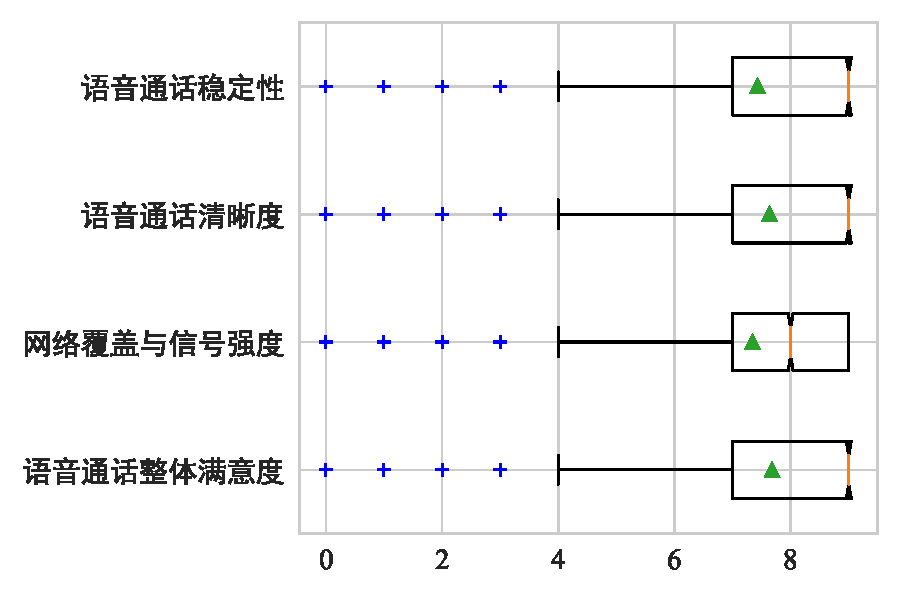
\includegraphics[width=1.0\linewidth]{[附件1][语音通话整体满意度、网络覆盖与信号强度、语音通话清晰度、语音通话稳定性]评分箱线图.pdf}
			\caption{语音业务用户四项评分箱线图}
			\label{fig:语音业务箱线图}
		\end{minipage}
		%\qquad
		\begin{minipage}{0.48\linewidth}
			\centering
			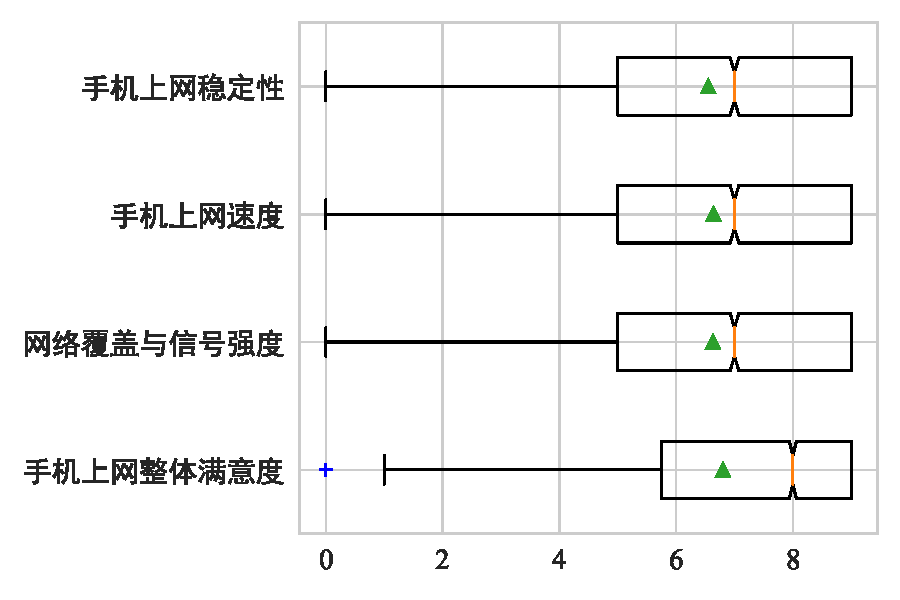
\includegraphics[width=1.0\linewidth]{[附件2][手机上网整体满意度、网络覆盖与信号强度、手机上网速度、手机上网稳定性]评分箱线图.pdf}
			\caption{上网业务用户四项评分箱线图}
			\label{fig:上网业务箱线图}
		\end{minipage}
	\end{figure}
	同时我们还绘制出用户对于语音及上网业务共计八项评分的皮尔逊相关系数热力图,如\textcolor{blue}{\cref{fig:语音业务热力图}}、\textcolor{blue}{\cref{fig:上网业务热力图}}所示。其中皮尔逊相关系数计算方法如下:
	\begin{equation}
		\rho\left(x,y\right)=\frac{\sum\limits_{i=1}^{n}\left(x_{i}-\mu_x\right)\left(y_{i}-\mu_y\right)}{\sqrt{\sum\limits_{i=1}^{n}\left(x_{i}-\mu_x\right)^{2}}\sqrt{\sum\limits_{i=1}^{n}\left(y_{i}-\mu_y\right)^{2}}} \label{fpearson}
		\end{equation}
	其中$\mu$计算见\textcolor{blue}{\eqref{fmean}}。
	
	由该定义,显然$\rho\in[-1,1]$。当$\rho>0$时,上述两变量呈正相关;当$\rho=0$时,上述两变量不相关;当$\rho<0$时,上述两变量呈负相关。当$\left|\rho\right|$越接近于$1$时,则上述两变量相关性就越强\textcolor{blue}{\cite{ppearson}}。
	\begin{figure}[H]
		\centering
		\begin{minipage}{0.48\linewidth}
			\centering
			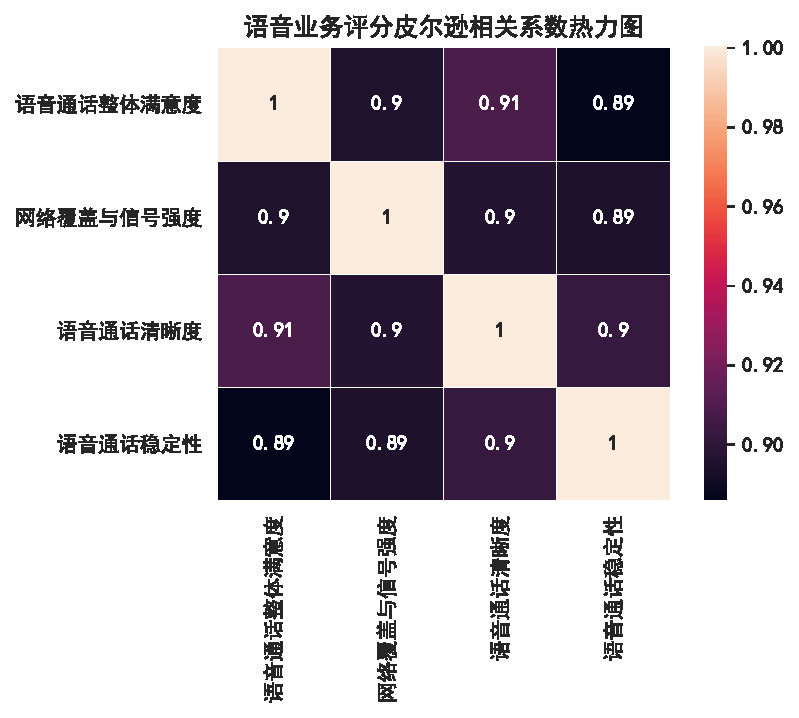
\includegraphics[width=1.0\linewidth]{[附件1]语音业务评分皮尔逊相关系数热力图.pdf}
			\caption{语音业务评分皮尔逊相关系数热力图}
			\label{fig:语音业务热力图}
		\end{minipage}
		%\qquad
		\begin{minipage}{0.48\linewidth}
			\centering
			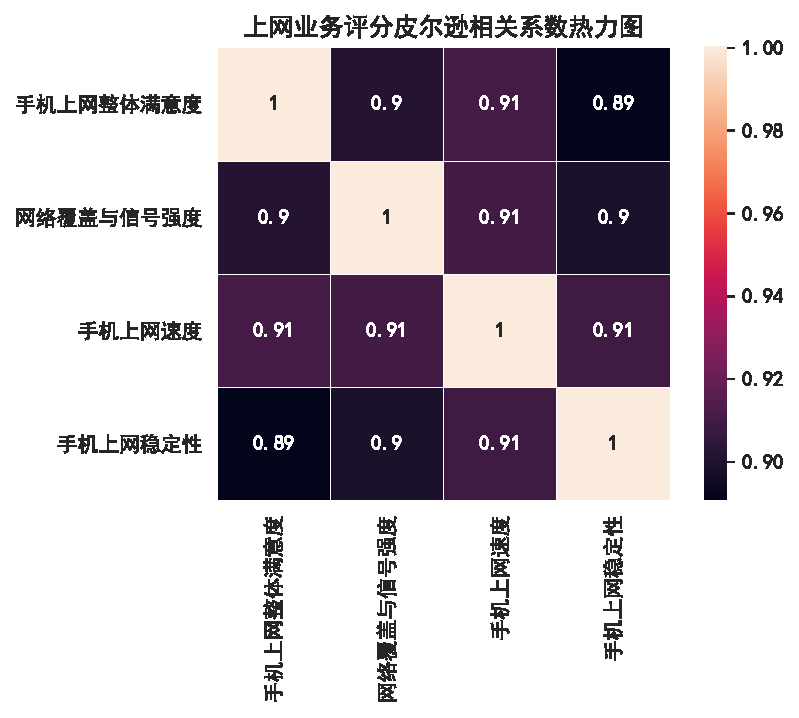
\includegraphics[width=1.0\linewidth]{[附件2]上网业务评分皮尔逊相关系数热力图.pdf}
			\caption{上网业务评分皮尔逊相关系数热力图}
			\label{fig:上网业务热力图}
		\end{minipage}
	\end{figure}
	依据对上图的分析,我们可以发现用户对于每一业务的四项评分,其分布规律大致一致,且皮尔逊相关程度高,数据内部差异较小。同时为了方便、快捷、高效地将评分数据分为高分组及低分组,为后续分析评分为高分及低分的用户的特征做好充足准备,本文对于两项业务的各四项评分取平均值且取整,得到用户对于该项业务的整体评分,这样处理好处有二:
	\begin{itemize}
		\item \textbf{降低评分维度,方便后续整体分析};
		\item \textbf{避免相似因素特征的重复分析,提高处理效率}。
	\end{itemize}

	得到语音及上网业务的“整体评分”后,我们依据实际情况,划定高分组、中间组、低分组评分,如\textcolor{blue}{\cref{tab:评分划定}}所示。
	\begin{table}[H]
	\centering
	\caption{低分组、中间组、高分组评分划定及结果}
	\scalebox{0.92}{
	  \begin{tabular}{cccc}
	  \toprule
	  \textbf{项目} & \textbf{低分组} & \textbf{中间组} & \textbf{高分组} \\
	  \midrule
	  整体评分  & 1、2、3、4、5 & 6、7   & 8、9、10 \\
	  语音业务用户数量/占比 & 413 / 7.61 \% & 1102 / 20.30 \% & 3913 / 72.09 \% \\
	  上网业务用户数量/占比 & 1005 / 14.32 \% & 2170 / 30.91 \% & 3845 / 54.77 \% \\
	  \bottomrule
	  \end{tabular}}
	\label{tab:评分划定}
  	\end{table}

	\subsection{用户评分分组特征分析}
	依据上述评分划定,我们划分用户评分的高分组、中间组及低分组,这里我们着重分析高分组及低分组用户的特征。
	\begin{itemize}
		\item \textbf{语音业务}:
		通过对比语音业务评分低分组和高分组的各项特征,我们可以发现:
		\begin{itemize}
			\item 低分组“脱网次数”“mos质差次数”“未接通电话次数”和“遇到过网络问题”的平均数普遍高于高分组,反映了在网络与信号质量方面评分低的用户普遍低于评分高的用户,用户使用感相对于评分高的用户更差,根据mos语音质量评价方法,说明低分组用户在语音通话的过程中存在较多听不太清,有较大的杂音和断续,失真严重的情况。
			\item 低分组出现“手机没有信号”“有信号无法拨通”“通话过程中突然中断”“通话中有杂音、听不清、断断续续”“串线”“通话过程中一方听不见”这些问题的次数明显高于高分组,同时低分组的1/2分位数及3/4分位数大多为1,而高分组的1/4,1/2,3/4分位数皆为0,说明在不考虑个别极端值的条件下,一般低分用户,即超过一半以上的低评分用户相较于高分用户大多存在语音通话中的各样的问题。
			\item 低分组“套外流量和费用”“外省流量占比”“GPRS总流量”“GPRS-国内漫游的流量”“当月ARPU”和“前3月MOU”的平均值皆高于高分组,说明评分低的客户对流量的使用和对手机依赖程度相较于评分高的用户更高,平均每个用户贡献的通信业务收入更多。
			\item 低分组“外省语音占比”“语音通话-时长”“省际漫游-时长”“当月MOU”和“前3月MOU”的平均值皆高于高分组,说明低分组在日常生活中手机通话次数与通话时长皆高于高分组,手机使用更为频繁。
			\item 在原数据集中,“居民小区”“办公室”“高校”“商业街”“地铁”“农村”“高铁”均为出现问题的场所,本文绘制出语音业务高分组与低分组场所二层饼图,其中外层为低分组,内层为高分组,如\textcolor{blue}{\cref{fig:语音业务高分组与低分组场所二层饼图}}所示。
			\begin{figure}[H]
				\centering
				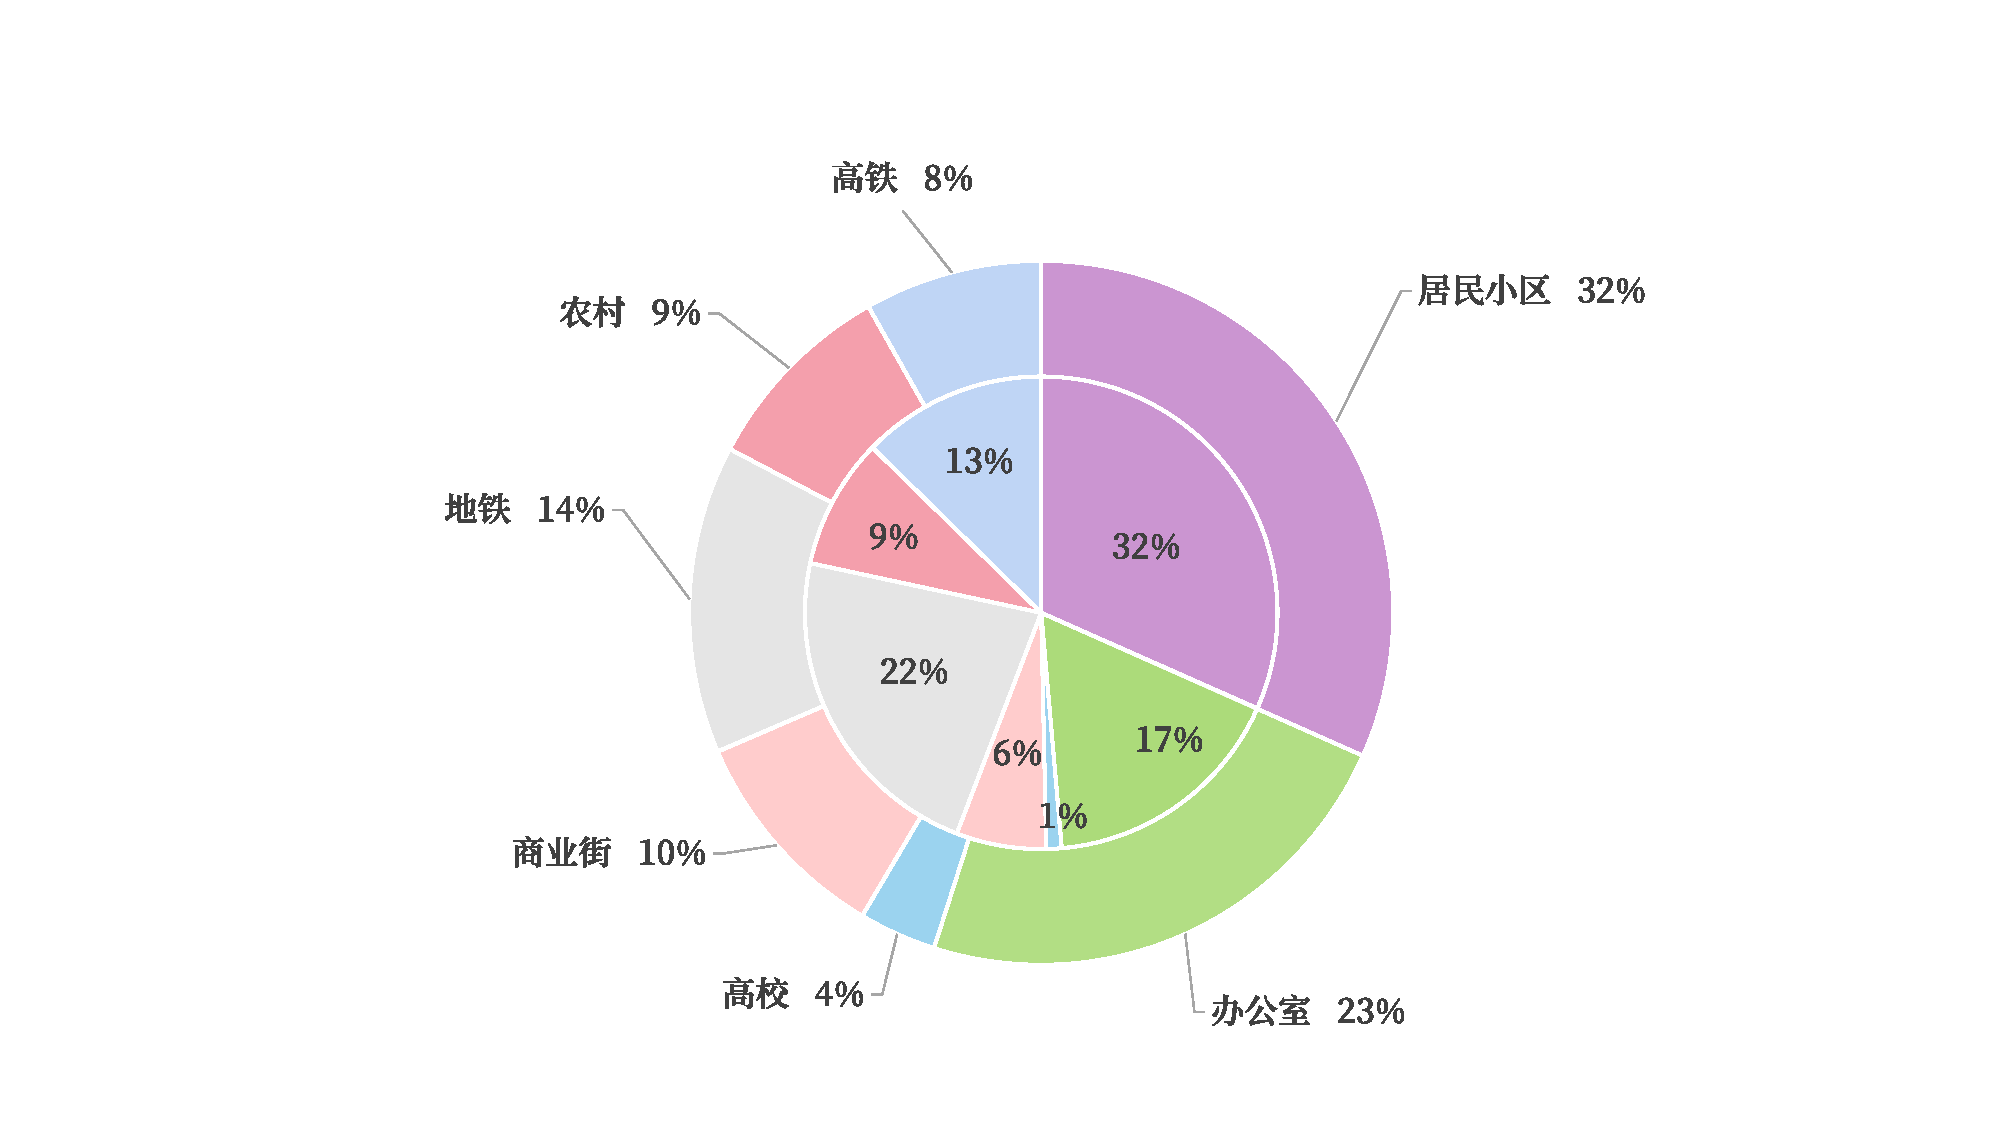
\includegraphics[width=0.48\textwidth]{语音业务二层饼图.pdf}
				\caption{语音业务高分组与低分组场所二层饼图}
				\label{fig:语音业务高分组与低分组场所二层饼图}
			\end{figure}
			观察上图,我们可以发现,无论是高分组还是低分组,其出现问题的场所大致相似,但更多用户在“高校”“办公室”“商业街”出现问题后,极有可能给出较低的评分。
			\item 在品牌方面,我们发现受调查用户大多均为苹果、华为手机,因此,这里我们统计低分组及高分组中各品牌手机用户占比,如\textcolor{blue}{\cref{tab:语音业务各手机品牌用户占比}}所示。
\begin{table}[H]
	\centering
	\caption{语音业务各手机品牌用户占比}
	\scalebox{0.92}{
	  \begin{tabular}{cccc}
	  \toprule
	  \textbf{分组} & \textbf{华为} & \textbf{苹果} & \textbf{其他} \\
	  \midrule
	  高分组   & 44.70 \% & 33.55 \% & 21.75 \% \\
	  低分组   & 20.58 \% & 61.74 \% & 17.68 \% \\
	  \bottomrule
	  \end{tabular}}
	\label{tab:语音业务各手机品牌用户占比}
\end{table}
			由上表,我们可以明显发现,对于语音业务,高分组用户使用的手机品牌多为“华为”,而低分组用户使用的手机品牌多为“苹果”。
			\item 在先前,本文提及到对于语音业务构造出的三列新数据集,分别为:“场所合计”“出现问题合计”“脱网次数、mos质差次数、未接通掉话次数合计”,我们分别绘制出高分组与低分组对应的散点分布图,在图示中,若散点颜色越深,则说明对应的指标数量也就越多。如\textcolor{blue}{\cref{fig:语音业务场所合计高分组}}\textasciitilde\textcolor{blue}{\cref{fig:语音业务脱网次数、mos质差次数、未接通掉话次数合计低分组}}所示。
			
			观察\textcolor{blue}{\cref{fig:语音业务场所合计高分组}}及\textcolor{blue}{\cref{fig:语音业务场所合计低分组}},我们可以发现:高分组用户“场所合计”指标明显少于低分组用户,且低分组用户“场所合计”指标中,展现出的用户群体呈现更分散化,这也说明低分组用户在日常生活中对于移动手机的使用更为频繁,且使用的场所环境更多元。

			观察\textcolor{blue}{\cref{fig:语音业务出现问题合计高分组}}及\textcolor{blue}{\cref{fig:语音业务出现问题合计低分组}},我们可以发现:高分组用户“出现问题合计”指标数值及用户群体明显少于低分组,且低分组用户“出现问题合计”分布更为离散,说明低分组用户在语音通话的过程中存在较多方面的不同的问题,如掉话、通话质量差等,而高分组用户遇到的不佳情况明显少于低分组用户,同时遇到的问题类型也更为单一。
			\begin{figure}[htbp]
				\centering
				\begin{minipage}{0.48\linewidth}
					\centering
					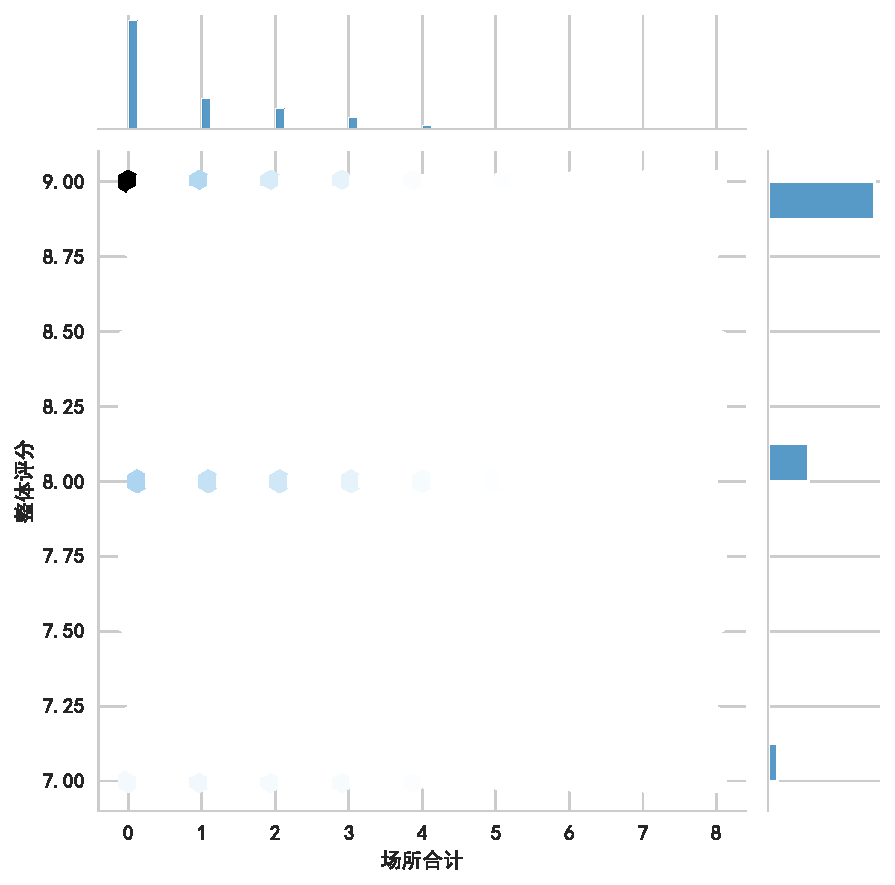
\includegraphics[width=0.70\linewidth]{[附件1]高分组场所合计分布情况.pdf}
					\caption{语音业务场所合计高分组散点分布图}
					\label{fig:语音业务场所合计高分组}
				\end{minipage}
				%\qquad
				\begin{minipage}{0.48\linewidth}
					\centering
					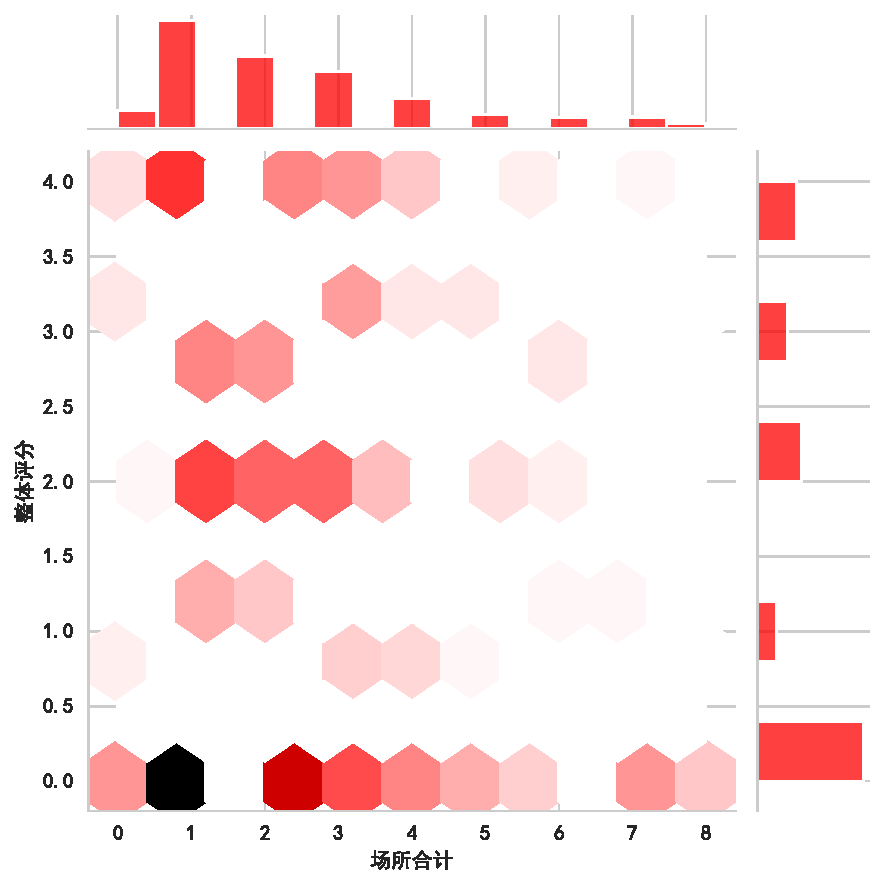
\includegraphics[width=0.70\linewidth]{[附件1]低分组场所合计分布情况.pdf}
					\caption{语音业务场所合计低分组散点分布图}
					\label{fig:语音业务场所合计低分组}
				\end{minipage}
			\end{figure}
			\begin{figure}[htbp]
				\centering
				\begin{minipage}{0.48\linewidth}
					\centering
					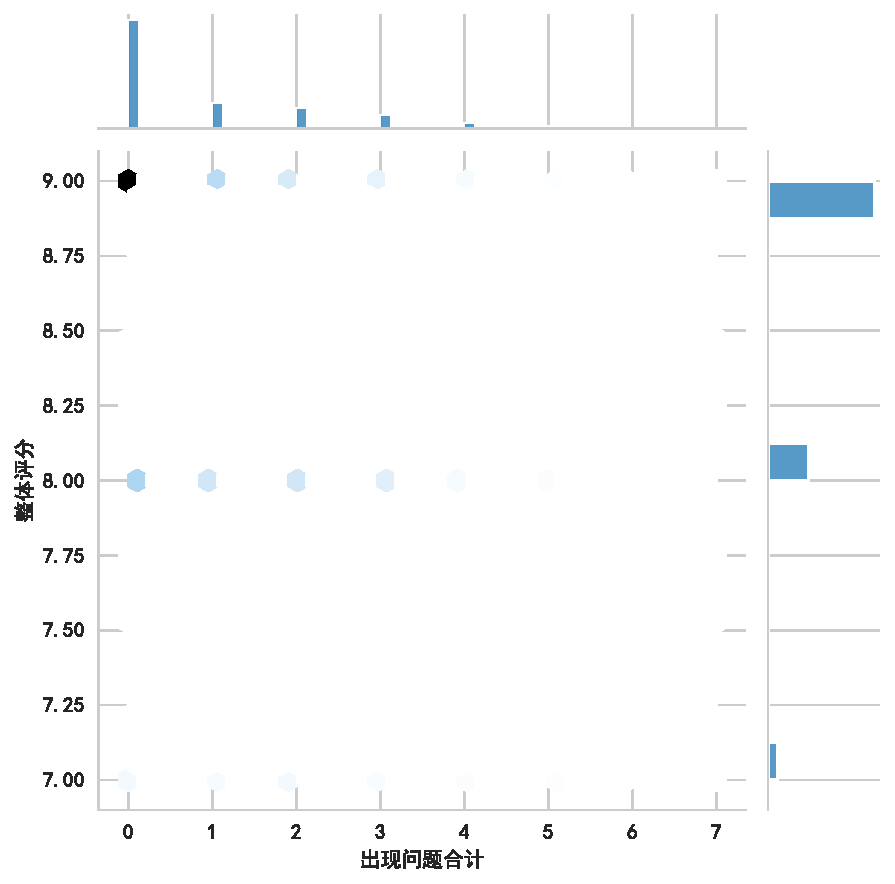
\includegraphics[width=0.70\linewidth]{[附件1]高分组出现问题合计分布情况.pdf}
					\caption{语音业务出现问题合计高分组散点分布图}
					\label{fig:语音业务出现问题合计高分组}
				\end{minipage}
				%\qquad
				\begin{minipage}{0.48\linewidth}
					\centering
					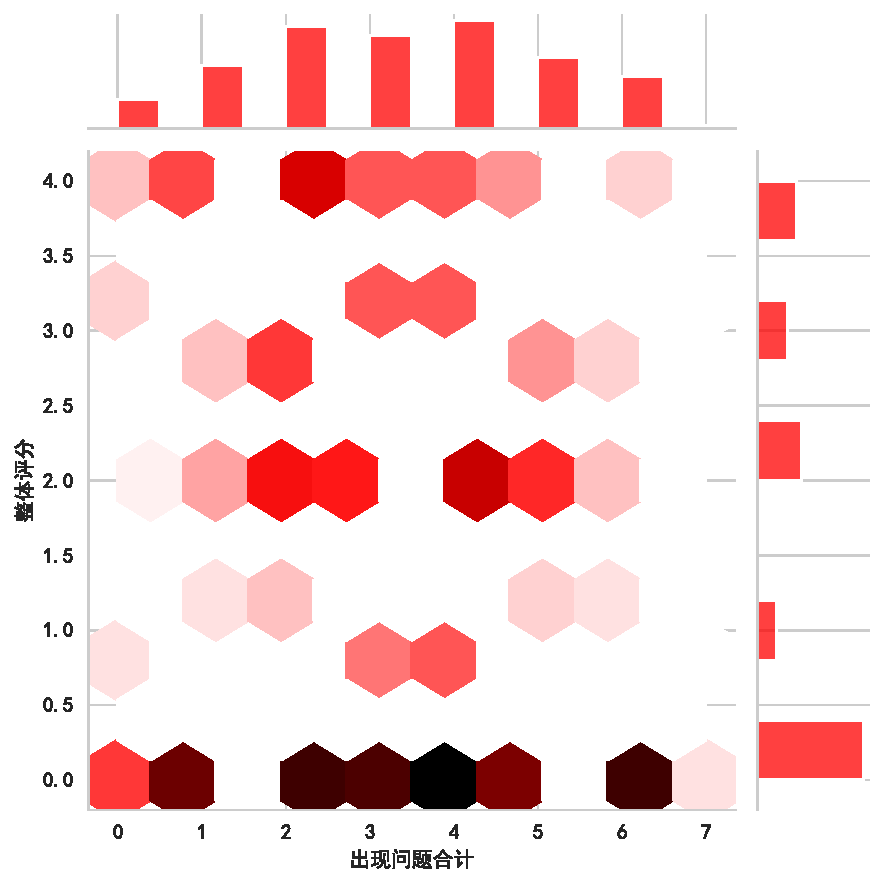
\includegraphics[width=0.70\linewidth]{[附件1]低分组出现问题合计分布情况.pdf}
					\caption{语音业务出现问题合计低分组散点分布图}
					\label{fig:语音业务出现问题合计低分组}
				\end{minipage}
			\end{figure}
			\begin{figure}[H]
				\centering
				\begin{minipage}{0.48\linewidth}
					\centering
					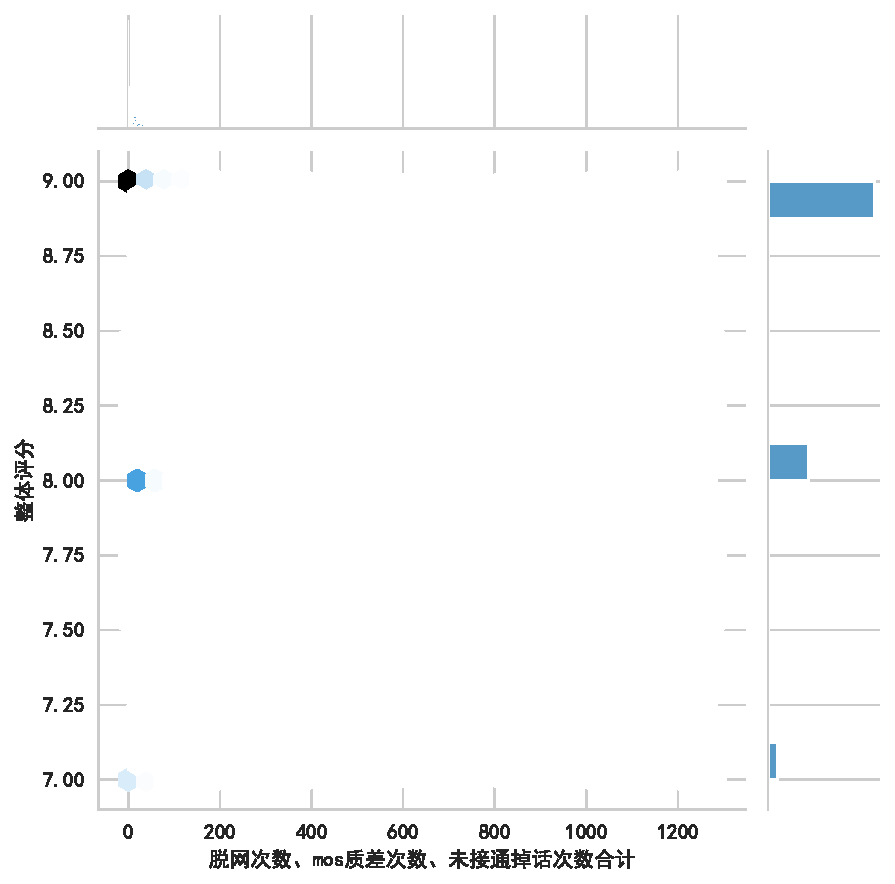
\includegraphics[width=0.70\linewidth]{[附件1]高分组脱网次数、mos质差次数、未接通掉话次数合计分布情况.pdf}
					\caption{语音业务不稳定情况高分组散点分布图}
					\label{fig:语音业务脱网次数、mos质差次数、未接通掉话次数合计高分组}
				\end{minipage}
				%\qquad
				\begin{minipage}{0.48\linewidth}
					\centering
					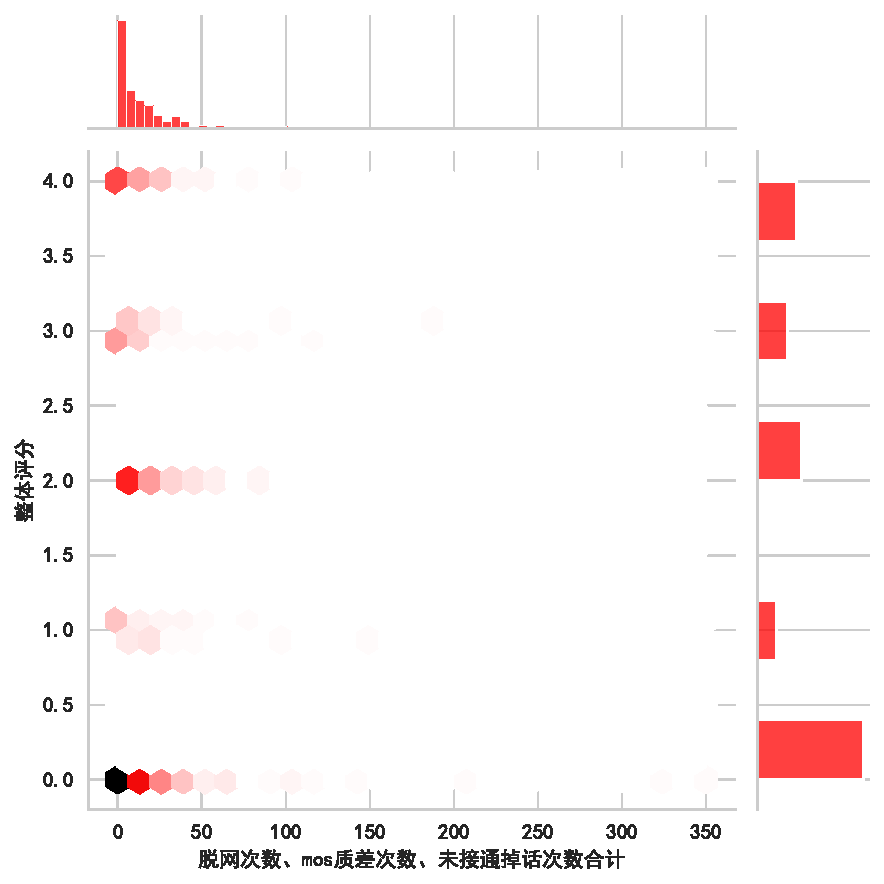
\includegraphics[width=0.70\linewidth]{[附件1]低分组脱网次数、mos质差次数、未接通掉话次数合计分布情况.pdf}
					\caption{语音业务不稳定情况低分组散点分布图}
					\label{fig:语音业务脱网次数、mos质差次数、未接通掉话次数合计低分组}
				\end{minipage}
			\end{figure}
		\end{itemize}
		观察\textcolor{blue}{\cref{fig:语音业务脱网次数、mos质差次数、未接通掉话次数合计高分组}}及\textcolor{blue}{\cref{fig:语音业务脱网次数、mos质差次数、未接通掉话次数合计低分组}},我们可以发现:高分组用户“语音业务脱网次数、mos质差次数、未接通掉话次数合计”次数在整体上明显少于低分组用户,且高分组用户在实际使用移动通信时,遇到的问题类型明显少于低分组用户,相反,低分组用户在整体上遇到的问题类型更多,对于单个用户,其在一定程度上,极有可能因遇到的问题类型较多,而给出较低评分。

		\item \textbf{上网业务}:通过对比上网业务评分低分组和高分组的各项特征,我们可以发现:
		\begin{itemize}
		\item 我们将用户上网满意度数据中针对软件的部分划分为视频类应用,游戏类应用,社交类应用,生活类应用四大类,通过对比评分高的用户与评分低的用户,对于这四大类应用,评分低用户的使用次数相较于评分高的用户更多,对手机软件的使用也更为频繁。
		\item 低分组出现“手机上网速度慢”“打游戏延时大”“显示有信号上不了网”“上网质差次数”“全部都卡顿全部游戏都卡顿”“脱网次数”“微信质差次数”“上网过程中网络时断时续或时快时慢”“打开网页或APP图片慢”“全部网页或APP都慢”“下载速度慢”“网络信号差/没有信号”“手机支付较慢”“和“看视频卡顿”这一系列网络问题的次数高于高分组,说明评分低的用户上网过程出现网络卡顿及不流畅的情况较多,网络整体质量较差,上网速度较慢;而评分高较少出现此类问题,上网过程更为清晰流畅。
		\item 在原数据集中,“居民小区”“办公室”“高校”“商业街”“地铁”“农村”“高铁”均为出现问题的场所,本文绘制出上网业务高分组与低分组场所二层饼图,其中外层为低分组,内层为高分组,如\textcolor{blue}{\cref{fig:上网业务高分组与低分组场所二层饼图}}所示。
		\begin{figure}[H]
			\centering
			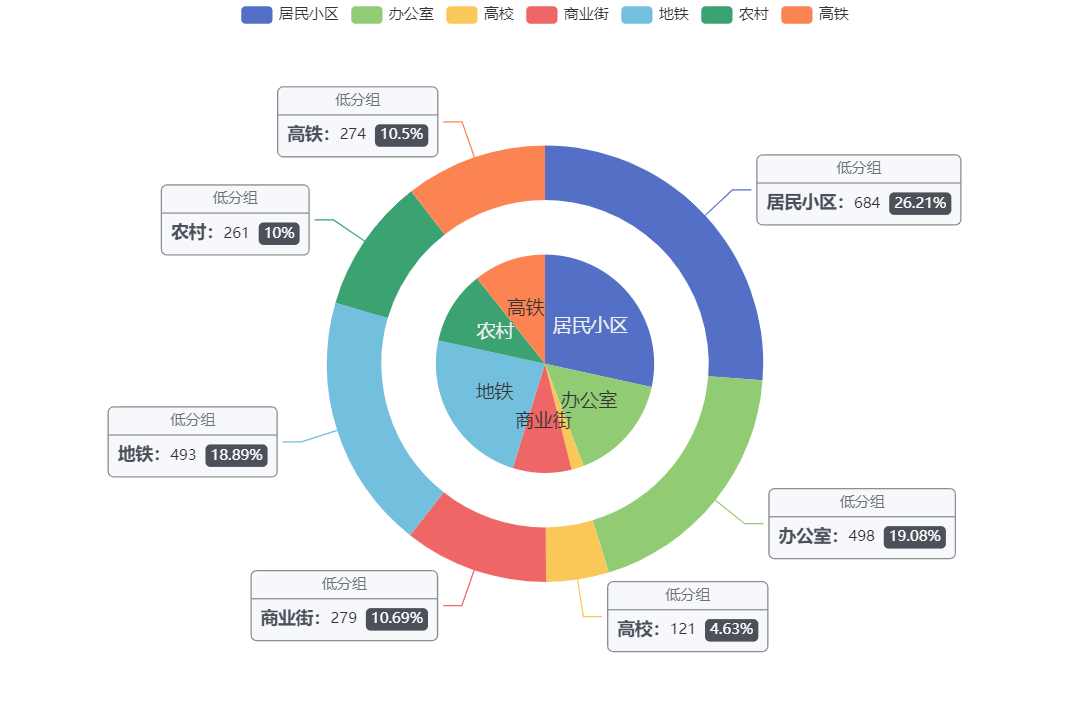
\includegraphics[width=0.70\textwidth]{上网业务地点.png}
			\caption{上网业务高分组与低分组场所二层饼图}
			\label{fig:上网业务高分组与低分组场所二层饼图}
		\end{figure}
		\item 在品牌方面,我们发现受调查用户大多均为苹果、华为手机,因此,这里我们统计低分组及高分组中各品牌手机用户占比,如\textcolor{blue}{\cref{tab:上网业务各手机品牌用户占比}}所示。
		\begin{table}[H]
			\centering
			\caption{上网业务各手机品牌用户占比}
			\scalebox{0.92}{
			  \begin{tabular}{cccc}
			  \toprule
			  \textbf{分组} & \textbf{华为} & \textbf{苹果} & \textbf{其他} \\
			  \midrule
			  高分组   & 41.59 \% & 29.36 \% & 29.05 \% \\
			  低分组   & 21.99 \% & 54.13 \% & 23.88 \% \\
			  \bottomrule
			  \end{tabular}}
			\label{tab:上网业务各手机品牌用户占比}
		\end{table}
		由上表,我们可以明显发现,对于上网业务,高分组用户使用的手机品牌多为“华为”,而低分组用户使用的手机品牌多为“苹果”。这与语音业务情况一致。
		\item 低分组“套外流量费”“套外流量”的平均值皆高于高分组,说明低分组在上网过程中使用流量的次数更多,同时对手机使用较为频繁以至于使用超出了流量套餐以外的费用较高。
		\item 在先前,本文提及到对于语音业务构造出的三列新数据集,分别为:“出现问题场所或应用总”“网络卡速度慢延时大上不了网总”“质差总”“地点总”,我们分别绘制出高分组与低分组对应的散点分布图\textcolor{blue}{\footnote{由于图幅与语音业务类似,且篇幅原因,本文将其放于附录[A]中,读者可自行查阅。同时下文多数图示由于篇幅过大且与在正文中展示的图示类似,故本文将部分图示放于附录[A]中,读者可自行查阅。}},在图示中,若散点颜色越深,则说明对应的指标数量也就越多。如\textcolor{blue}{\cref{fig:上网业务高分组问题及场所分布}}\textasciitilde\textcolor{blue}{\cref{fig:上网业务低分组地点分布}}所示。
		
		观察上述图示,我们可以发现:对于上网业务,低分组用户在日常生活中使用移动网络时,会在各主要场所,如“高校”“地铁”“办公室”等地点遇到各种类型的网络问题,且遇到的次数在整体上明显多于高分组用户;同时低分组用户及高分组用户都遇到质差问题。
	\end{itemize}
	\end{itemize}
	
	\subsection{用户评分合理性分析}
	
	为了更清晰地发现及描述各评分之间的散点关系,我们在此基础上绘制语音及上网业务的评分联合分布图,如\textcolor{blue}{\cref{fig:语音业务联合分布图}}、\textcolor{blue}{\cref{fig:上网业务联合分布图}}所示。
	\begin{figure}[H]
		\centering
			\centering
			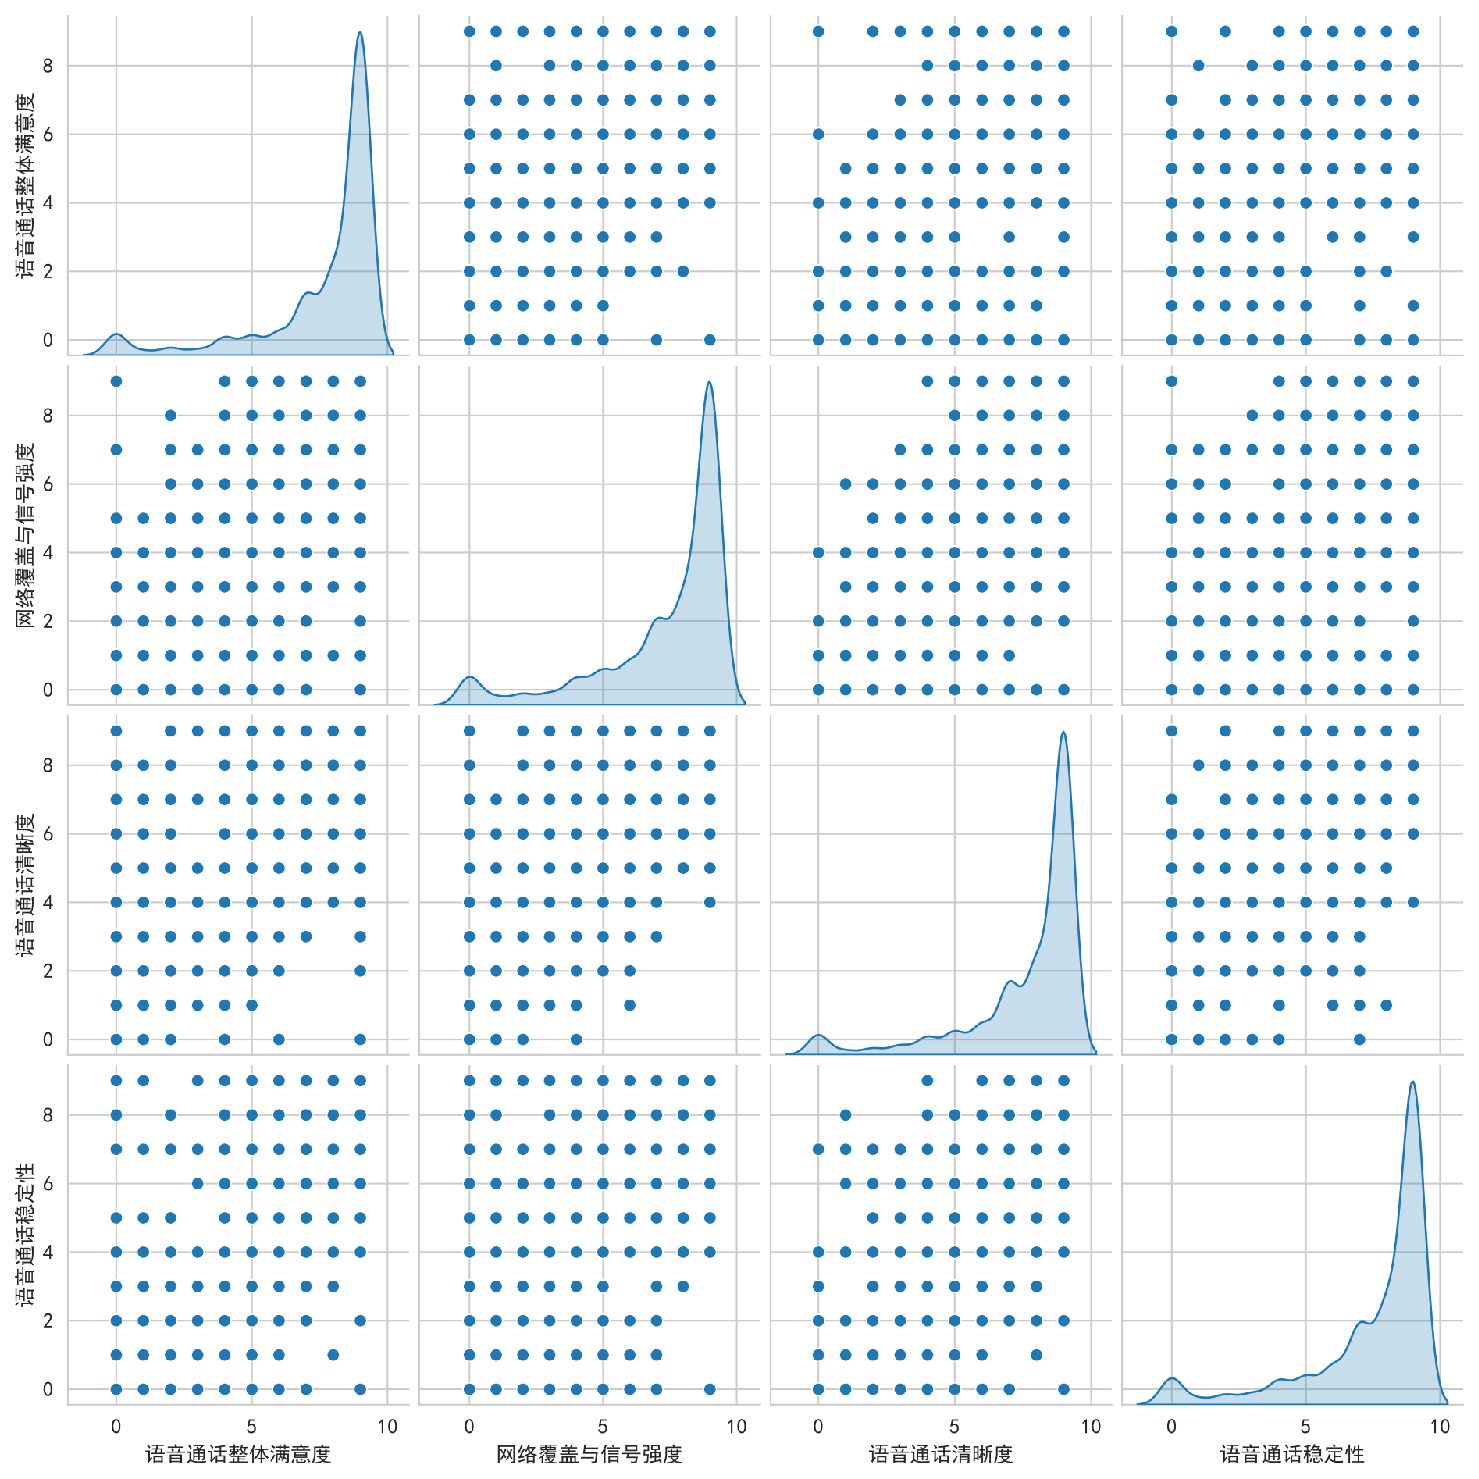
\includegraphics[width=0.66\linewidth]{[附件1][语音通话整体满意度、网络覆盖与信号强度、语音通话清晰度、语音通话稳定性]评分联合分布图_纯图版.pdf}
			\caption{语音业务用户四项评分联合分布图}
			\label{fig:语音业务联合分布图}
	\end{figure}

	观察\textcolor{blue}{\cref{fig:语音业务联合分布图}},我们可以发现其主对角线图示分别为语音业务中“语音通话整体满意度”、“网络覆盖与信号强度”、“语音通话清晰度”、“语音通话稳定性”四项评价指标的用户评分直方图,我们可以发现用户的评分在区间的两侧部分出现了两次极值,并结合实际考虑,利用上述四项评分的数据绘制联合分布图,即确定一项用户评分可得出其余三项用户评分的分布区间,由于评分中间的用户评分基数较小,故我们主要选取评分两侧分布更为集中,基数更大的用户评分区间进行分析,通过分布图我们可以看出在图的右下和左上两部分用户评分的分布更为分散,可视为离群点。例如我们选取语音通话整体满意度为1时的情况,对应的网络覆盖与信号强度出现了评分为10的情况,通过计算出同一用户对于不同的评价指标评分的极大值和极小值,若两者之间的差值超过了一定的阈值,即评分相差较大,便可以看做用户评分合理性较低的数据对此进行剔除以提升用户评分数据的准确度和合理性。
	
	观察\textcolor{blue}{\cref{fig:上网业务联合分布图}},我们可以发现用户评分的集中区间与直方图的趋势变化与语音业务用户评分大体相同,并出现了一次较小的峰值在评分为8的部分。于是,同语音业务分析一致,选取两侧用户评分的数据作为我们的主要分析对象,通过观察可以发现离群点同语音业务出现在图的右下,左上两个部分,但相比较与语音业务联合分布图,出现离群点的范围与个数有所缩小,但仍存在同一用户对于不同维度评价指标评分差异较大的现象,对此我们同样进行剔除处理以提升模型预测的效果。

	此外,我们还绘制出语音及上网业务的整体评分的低分组及高分组与前文我们提及到的特征因素的联合分布直方、散点图,如\textcolor{blue}{\cref{fig:语音业务高分组评分及特征多变量联合分布图}}\textasciitilde\textcolor{blue}{\cref{fig:上网业务低分组评分及特征多变量联合分布图}}所示。结合前文高分组与低分组用户特征的分析,我们可以发现,在数据集中存在少量用户实际体验与其评分结果相差较大,下文,本文将提出剔除不合理评分的依据及措施。

	\subsection{新数据集的建立}
	根据上述分析,我们对不合理用户的评分数据进行剔除,主要标准如下:
	\begin{itemize}
		\item 用户每一业务四项评分之间的差值若超过设定阈值即剔除,在这里,对于语音业务,我们设定“语音通话整体满意度”与“网络覆盖与信号强度”之间差值的阈值为5,“语音通话整体满意度”与其余两项评分之间的差值的阈值为4,“语音通话清晰度”与“语音通话稳定性”评分之间的差值的阈值为3;对于上网业务,我们设定“手机上网整体满意度”与“网络覆盖与信号强度”之间差值的阈值为5,“手机上网整体满意度”与其余两项评分之间的差值的阈值为4,“手机上网速度”与“手机上网稳定性”评分之间的差值的阈值为3;
		\item 同时也应考虑到非数字类型数据,即附件中“其他,请注明”列数据,在初赛中我们利用其绘制出用户提及高频词汇云图,发现该数据存在利用价值,因此本文有理由认为,若某一用户数据中有效存在该数据内容,即认为该用户对于该业务的评分合理;
		\item 此外,通过上述对各业务高分组及低分组用户行为特征的分析,我们针对部分少量用户不符整体行为特征的用户进行剔除,保证训练数据集的纯度;
		\item 这里,我们主要对高分组与低分组用户进行合理性分析,并对该两组不合理情况进行剔除,而对于中间组评分用户,我们认为其评分合理性较高,故不对其进行剔除。
	\end{itemize}
	
	依据上述剔除标准,我们对原数据集进行合理性剔除,剔除结果如\textcolor{blue}{\cref{tab:剔除结果}}所示。\textbf{注:原数据集用户量是经过数据预处理后得到的数量。}
\begin{table}[H]
	\centering
	\caption{数据集合理性剔除结果}
	  \begin{tabular}{ccccc}
	  \toprule
	  \textbf{业务类型} & \textbf{原数据集用户量} & \textbf{被剔除用户量} & \textbf{新数据集用户量} & \textbf{合理用户量占比} \\
	  \midrule
	  语音业务  & 5428  & 115   & 5313  & 97.88 \% \\
	  上网业务  & 7020  & 202   & 6818  & 97.12 \% \\
	  \bottomrule
	  \end{tabular}
	\label{tab:剔除结果}
\end{table}
\textbf{后文模型的建立将在新数据集上进行,此外,本文也将会将新数据集上建立的模型效果与初赛模型效果进行对比,分析预测合理性。}
	\subsection{多分类模型的建立}
	本文依旧采用初赛使用的六种多分类模型,并对其进行Stacking集成学习。首先多分类基本模型建立理论如下:
	\begin{itemize}
		\item \textbf{随机森林(Random Forest, RF)}是由多棵决策树(Decision Tree)进行组合后对预测结果投票或取均值的一种算法\textcolor{blue}{\cite{prf}}。其有分类和回归两种模型,对于本题,我们选择分类模型。其简要过程如\textcolor{blue}{\cref{fig:RF}}所示,算法伪代码如\textcolor{blue}{Algorithm\ref{RFfunction}}所示。

		\begin{figure}[H]
			\centerline{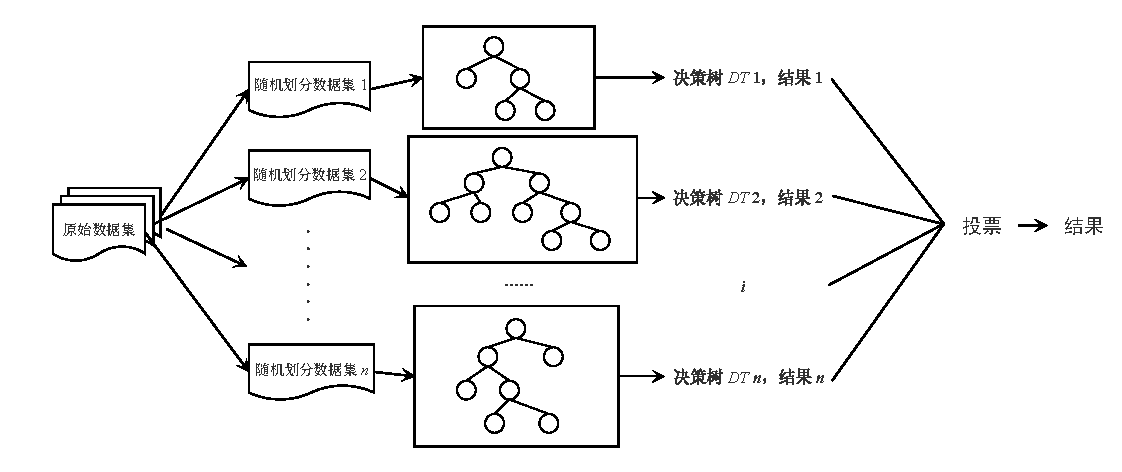
\includegraphics[scale=0.66]{随机森林简图.pdf}}
			\caption{随机森林算法简图}\label{fig:RF}
		\end{figure}
		
		对于单棵决策树而言,本文利用\textbf{CART}算法\textcolor{blue}{\cite{prf}}构建。基尼系数是衡量样本集合纯度的指标,当该值越小时,其纯度也就越高。计算公式如下
		\begin{equation}
			Gini\left( R_i \right)=\sum\limits_{k=1}^{K}\sum\limits_{k\ne k'}P_k P_{k'}=1-\sum\limits_{k=1}^{K}P_k^2 \label{fGini}
		\end{equation}
		其中,$R$为选取出的特征(影响因素),$K$表示在该特征中包含的类别数,$P_k$表示该特征中第$k$类别的出现概率。
	
		由上述分析可知,对于单棵决策树而言,其叶子节点的分裂特征为选择的所有特征中基尼系数最小的特征。

		\scalebox{0.88}{
		\begin{algorithm}[H]
			\label{RFfunction}
			\KwData{数据集$\mathcal{D}$}
			\textbf{function} DTree$\left(\mathcal{D}\right)$\
			
			\eIf{Termination}
			{\textbf{return} $\mathrm{base}\left(g_t\right)$}
			{\textbf{learn} $b\left(x\right)$并且依据$b\left(x\right)$划分$\mathcal{D}$为$\mathcal{D}_C$\
	
			\textbf{build} $G_C \leftarrow$ DTree($\mathcal{D}_C$)\
	
			\textbf{return} $G\left(x\right)=\sum\limits_{C=1}^{C}[\![b\left(x\right)=C]\!]G_C\left(x\right)$}
			
			\textbf{function} RandomForest$\left(\mathcal{D}\right)$\
			
			\For{$t=1,2,3,\cdots,T$}{\textbf{request} 数据集$\tilde{\mathcal{D}}_t \leftarrow$ BoostStrapping$\left(\mathcal{D}\right)$\
			
			\textbf{obtain} DTree $g_t\leftarrow$ DTree$\left(\tilde{\mathcal{D}}_t\right)$\
	
			\textbf{return} $G=$ Uniform$\left(g_t\right)$
			}
			
			\KwResult{随机森林模型$G=\mathrm{Uniform}\left(g_t\right)$}
			\caption{随机森林(RF)}
		\end{algorithm}}

		\item \textbf{极端梯度提升(eXtreme Gradient Boosting, XGBoost)}。XGBoost算法是一种基于树模型的优化模型,其将弱分类器组合,训练出一个较强的分类器。该算法通过多次迭代,生成一个新的树模型用于优化前一个树模型,随着迭代次数的增多,该模型的预测精度也会相应提高\textcolor{blue}{\cite{pxgboost1}}。

		记通过数据处理后的数据集特征为$R\left(x_{ij}\right)_{m\times n}$,表示其包含$m$个用户,$n$个特征,在训练中形成的CART树的集合记为$F=\left\{f\left(x\right)=w_{q\left(x\right)},q:\mathbf{R}^n\to T,w\in \mathbf{R}^T\right\}$,其中$q$为树模型的叶节点决策规划,$T$为某一树模型叶节点数量,$w$为叶节点对应的得分\textcolor{blue}{\cite{pxgboost2}}。对于预测的$y$值,其计算公式为
		\begin{equation}
			\hat{y}=\varphi \left( x_i \right) =\sum\limits_{k=1}^K{f_k\left( x_i \right)} \label{fXGBoostypre}
		\end{equation}
	
		XGBoost算法在每一次迭代过程中会保存前面所学习的模型,会将这些模型加入到新一轮迭代过程中,因此我们记第$i$个模型为预测结果为
		\begin{equation}
			\hat{y}_{i}^{\left(t\right)}=\hat{y}_{i}^{\left(t-1\right)}+f_t\left(x_i\right) \label{fXGBoostyprei}
		\end{equation}
		
		XGBoost算法的目标函数计算公式如下
		\begin{equation}
			L^{\left(t\right)}=\sum\limits_{i=1}^{n}l\left(y_i,\hat{y}_{i}^{\left(t-1\right)}+f_t\left(x_i\right)\right)+\gamma T+\frac{1}{2}\lambda\sum\limits_{j=1}^T{w_j^2}+\mathrm{const} \label{fXGBoostL}
		\end{equation}
		% 其中
		% \begin{equation}
		% 	\Omega\left(f_t\right)=\gamma T+\frac{1}{2}\lambda\sum\limits_{j=1}^T{w_j^2} \label{fXGBoostOmega}
		% \end{equation}
		上述公式中,$l$为模型误差损失,描述在该模型下预测值与实际值之间的出差异损失,$\Omega$为模型叶节点的正则项惩罚系数,$\gamma$与$\lambda$为模型的超参数\textcolor{blue}{\cite{pxgboost2}}。
		通常情况下,我们难以用枚举法得到在模型中所训练出来的树结构,因此这里采用贪婪算法,从单叶子节点开始,通过迭代方法,将其加入到树结构中,从而得到最优解,其计算公式\textcolor{blue}{\cite{pxgboost3}}如下
		\begin{equation}
			\mathcal{L}_{split}=\frac{1}{2}\left[\frac{\left(\sum_{i\in I_L}g_i\right)^2}{\sum_{i\in I_L}h_i+\lambda}+\frac{\left(\sum_{i\in I_R}g_i\right)^2}{\sum_{i\in I_R}h_i+\lambda}-\frac{\left(\sum_{i\in I}g_i\right)^2}{\sum_{i\in I}h_i+\lambda}\right]-\gamma \label{fXGBoostLsplit}
		\end{equation}
		其中$I_j=\left\{i|q\left(x_i\right)=j\right\}$为叶节点$j$上的样本集合\textcolor{blue}{\cite{pxgboost2}},且有
		\begin{equation}
			g_i=\partial_{\hat{y}^{\left(t-1\right)}}l\left(y_i,\hat{y}_i^{\left(t-1\right)}\right)
		\end{equation}
		\begin{equation}
			h_i=\partial_{\hat{y}^{\left(t-1\right)}}^2l\left(y_i,\hat{y}_i^{\left(t-1\right)}\right) \label{xgboosthi}
		\end{equation}
	
		通过上述分析,我们可以得到XGBoost算法简图,如\textcolor{blue}{\cref{fig:XGBoost}}所示。
		\begin{figure}[h!t]
			\centerline{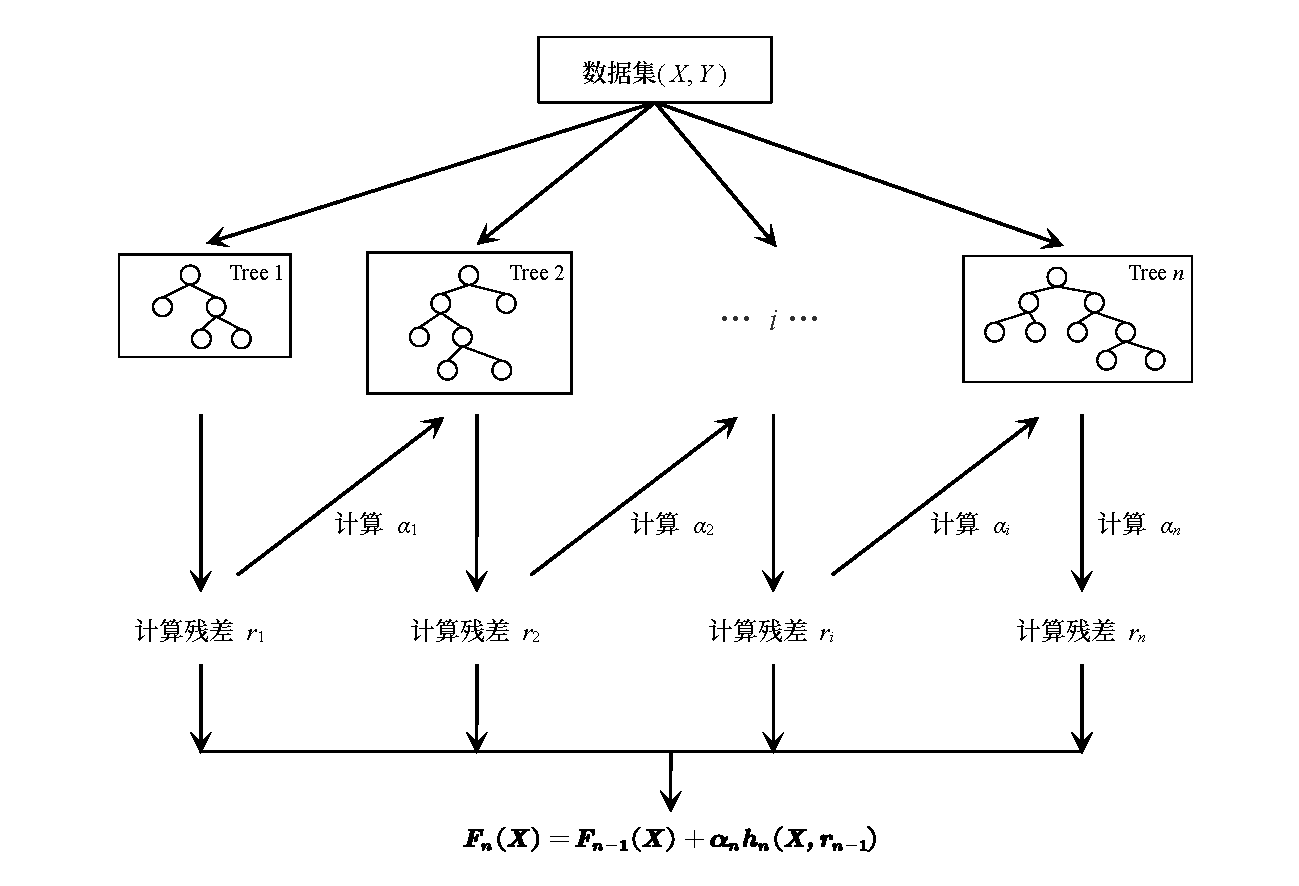
\includegraphics[scale=0.56]{XGBoost简图.pdf}}
			\caption{XGBoost算法简图}\label{fig:XGBoost}
		\end{figure}
		\item \textbf{K-近邻(K Nearest Neighbor, KNN)}。KNN算法的主要思想为:在出现新样本时从现有的训练数据中找到与其相对应的最接近的$K$个样本,并根据最相似的类别出现的样本进行分类。基于多数$K$个样本所属的类别来分辨待分类的数据集所属的类别\textcolor{blue}{\cite{pknn}}。接近度由两点之间的距离函数给出属性空间中的点决定。距离函数通常使用两个点之间的标准欧几里得距离。欧氏距离的计算公式如下
		\begin{equation}
			d(X, Y)=\sqrt{\sum\limits_{i=1}^{n}\left(X_{i}-Y_{i}\right)^{2}} \label{fdistance}
		\end{equation}
		其中$X=\left(x_{1},x_{2},\cdots,x_{m}\right)^{\mathrm{T}}$和$Y=\left(y_{1},y_{2},\cdots,y_{m}\right)^{\mathrm{T}}$表示两个样本列数据,$m$为样本数量。
		
		\item \textbf{支持向量机(Support Vector Machine, SVM)}。SVM建立在结构风险最小原理及Vapnik-Chervonenkis理论基础之上\textcolor{blue}{\cite{psvm}},以有限的数据信息,在数据样本中找出合适区分类别的决策分界面,且保证边界点与分界面尽可能远,即需要再找出合适的边界分界面,该算法示意图如\textcolor{blue}{\cref{fig:svmpicture}}所示。
		\begin{figure}[h!t]
			\centerline{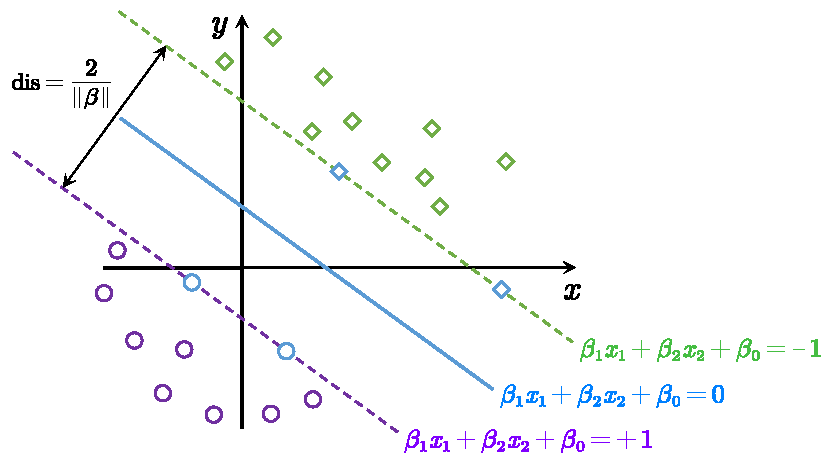
\includegraphics[scale=0.60]{SVM示意图.pdf}}
			\caption{SVM示意图}\label{fig:svmpicture}
		\end{figure}
		而由于SVM多应用于解决二分类问题,且我们需要建立多分类模型,因此需要对其进行相应的改进。本文采用OVR(One Versus Rest)方法,将该问题改进为多个二分类问题\textcolor{blue}{\cite{psvm}}。在模型的训练时,任意将某一类别记为一类,其余类别记为另一类别,依次下去,建立出多分类的SVM模型。而对于核函数的选择,本文选择高斯核函数进行求解,其定义公式如下
		\begin{equation}
			K\left(x_i, x_j\right)=\exp \left(-\frac{\left\|x_i-x_j\right\|^{2}}{2\sigma^{2}}\right)=\exp \left(-\gamma \left\|x_i-x_j\right\|^{2}\right) \label{fgauss}
		\end{equation}
		对于高斯核函数,其可以反映出样本两点之间的相似度大小。当$\sigma$确定后,若两点之间距离越小,则相似度趋近于1;若距离越大,则相似度趋近于0。
		\item \textbf{LightGBM(Light Gradient Boosting Machine)}。LightGBM模型是基于决策树算法构建的一种高效的机器学习算法\textcolor{blue}{\cite{plightgbm}}。其为XGBoost、直方图算法(Histogram)、基于梯度的单边采样(GOSS)算法以及互斥特征捆绑(EFB)算法的结合的一种算法。
		
		\item \textbf{多分类逻辑回归(Multinomial Logistic Regression)}。多分类逻辑回归是基于逻辑回归(Logistic Regression)进行学习的分类模型。对于逻辑回归模型,其属于分类模型,多用于二分类问题。若数据集为$\left(\boldsymbol{A},\boldsymbol{B}\right)=\left(\left(\boldsymbol{a}_1,b_1\right),\left(\boldsymbol{a}_2,b_2\right),\cdots,\left(\boldsymbol{a}_m,b_m\right)\right)^{\mathrm{T}}$,其中$\boldsymbol{a}_i=\left(a_i^1,a_i^2,\cdots,a_i^j\right)$,$a_i^j$为样本$\boldsymbol{a}_i$的第$j$个特征,$\boldsymbol{B}$为因变量标签矩阵,该模型使用Sigmoid函数,同时构建样本$\boldsymbol{a}_i$所属类别的概率,对于标签为$1$的结果,其概率可写为
		\begin{equation}
			P\left(b_i=1\mid \boldsymbol{a}_i,\boldsymbol{\omega}\right)=\frac{1}{1+\mathrm{e}^{-\boldsymbol{a}_ib_i\boldsymbol{\omega}^\mathrm{T}}} \label{fLRp}
		\end{equation}
		其中$\boldsymbol{\omega}=\left(\omega^0,\omega^1,\cdots,\omega^n\right)^\mathrm{T}$为权重向量,即为优化模型的超参数。
		逻辑回归中利用损失函数来评估模型的预测结果与实际值之间的误差,其计算公式如下
		\begin{equation}
			L\left(\boldsymbol{A},\boldsymbol{B},\boldsymbol{\omega}\right)=\frac{1}{m}\sum\limits_{i=1}^{m}\log \left(1+\mathrm{e}^{-\boldsymbol{a}_ib_i \boldsymbol{\omega}^{\mathrm{T}}}\right) \label{fLRl}
		\end{equation}
		而对于$\boldsymbol{\omega}$,常采用梯度下降法来获得模型参数的最优解,其通过
		\begin{equation}
			\boldsymbol{\omega}^{\alpha+1}=\boldsymbol{\omega}^\alpha-\frac{\gamma}{m}\sum\limits_{i=1}^{m}\left(\frac{1}{1+\mathrm{e}^{-\boldsymbol{a}_ib_i \boldsymbol{\omega}^{\mathrm{T}}}}-1\right)\boldsymbol{a}_ib_i \label{fLRw}
		\end{equation}
		进行迭代更新,其中$\gamma$为模型的学习率,当$\left|  \boldsymbol{\omega}^{\alpha}-\boldsymbol{\omega}^{\alpha+1} \right|<\eta$或达到最大迭代次数时,停止训练,输出最终模型,其中$\eta$为人为给定的阈值\textcolor{blue}{\cite{plr}}。
	\end{itemize}

	建立好上述六种多分类模型后,我们依据各模型的预测准确率、平均绝对误差、均方误差,建立Stacking集成学习,将上述模型有目的地进行合理组合,从各模型中学到优点,有利于模型的效果的提升。其基本过程为,首先将已经经过处理的原数据集划分成若干个子集数据,在第一层建立多个模型的融合模型,输入数据,并采用五折交叉验证,获得每个模型的对于因变量标签的预测结果;之后第一层的输出结果作为第二层较弱分类模型的输入数据,第二层单个模型进行训练学习,得到最终预测结果\textcolor{blue}{\cite{pstacking}}。算法示意图如\textcolor{blue}{\cref{fig:StackingPicture}}所示,算法伪代码如\textcolor{blue}{Algorithm\ref{StackingFunciton}}所示。

	\scalebox{0.88}{
	\begin{algorithm}[H]
		\label{StackingFunciton}
		\KwIn{训练集$\mathcal{D}$\

		第一层学习模型$\mathcal{F}_1$,$\mathcal{F}_2$,$\cdots$,$\mathcal{F}_n$\

		第二层学习模型$\mathcal{S}$}
		\For{$t=1,2,3,\cdots,n$}{$h_n=\mathcal{F}_n\left(\mathcal{D}\right)$}
		$\mathcal{D}'=\varnothing$\

		\For{$i=1,2,\cdots,m$}{\For{$t=1,2,\cdots,n$}{$z_{in}=h_n\left(x_i\right)$}
		$\mathcal{D}'=\mathcal{D}'\cup\left(\left(z_{i1},z_{i2},\cdots,z_{in}\right),y_i\right)$}
		$h'=\mathcal{S}\left(D'\right)$

		\KwOut{$\mathcal{H}\left(x\right)=h'\left(h_1\left(x\right),h_2\left(x\right),\cdots,h_n\left(x\right)\right)$}
		\caption{Stacking集成学习}
	\end{algorithm}}
	\begin{figure}[H]
		\centerline{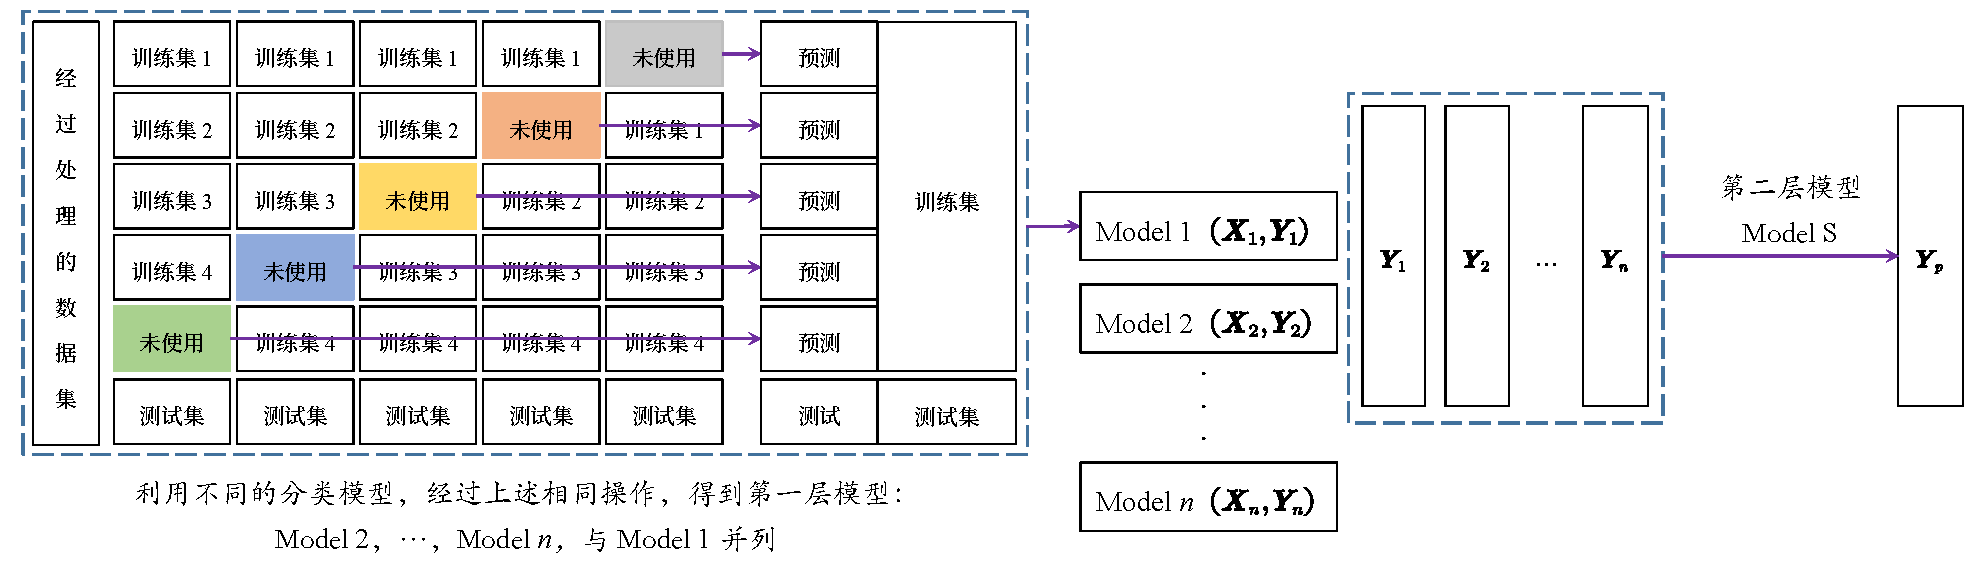
\includegraphics[scale=0.50]{Stacking示意图.pdf}}
		\caption{Stacking集成学习示意图}\label{fig:StackingPicture}
	\end{figure}
	\subsection{用户评分预测}
	在“5.1 相关准备工作”中,我们提到对学习数据与预测数据进行一致化,这是为了统一预测的自变量,避免不同的自变量的混乱,导致预测错误。经过对预测数据集的处理,利用上述已建立好的八个模型,对每一位用户的评分进行预测。这里我们需要注意的是:首先,要保证传入模型的变量要与训练时传入的指标一致;其次,在上文中我们提到我们选用多分类解决,而需要对评分进行标签编码,即将原评分$y\in\left[1,10\right]$映射至新评分标签$y'\in\left[0,9\right]$,即有关系式$y'=y-1$,而对于新数据的预测,我们要在模型的每个预测结果上加$1$,避免预测结果出错。由于被预测用户过多,我们将不在论文中展示,而将以文件形式保存至“附件6:result.xlsx”。
	
	\subsubsection{模型预测结果合理性分析}
	本文对于数据集充分分析,多方面考虑,首先对高分组与低分组评分用户分类讨论,分析及研究其主要特征;之后,我们依据整体用户行为进行分析,筛选出评分较为合理的用户群体作为新的数据集,并建立多模型调参融合的Stacking集成学习模型,且对模型训练采用五折交叉验证,保证模型的稳健性。对于语音业务数据的处理,我们将数据集划分训练集与测试集,比例为8:2;对于上网业务数据的处理,我们将数据集划分训练集与测试集,比例为9:1。对于两项业务这样处理有以下几点原因:
	\begin{itemize}
		\item 由于本题为用户对于移动公司语音及上网业务的评分预测,但该评分选择性较大且主观性强烈,难以以合理的量值确定用户对于该项业务的满意程度,因此仅能从整体用户行为中进行分析,分析出在整体用户中存在的部分”离群点“,即评分存在不合理的用户群体,从而对其进行剔除,在一定程度上保持样本数据的纯性,提升模型对于整体用户的预测准确性;
		\item 为验证模型的效果、分析模型的合理性、对模型参数进行调优、有监督地在数据上进行学习,更好地分析模型对于重要特征的选择,进行特征选择等,因此我们需要对数据集划分训练集与测试集;
		\item 对于语音业务,我们划分训练集与测试集比例为8:2,这是由于我们观察到,语音业务的数据分布较优,且需要学习的特征相对于上网业务较少,若过分提高该比例,模型可能会产生过拟合的情况,无法对未知数据进行高效分析,泛化能力差;
		\item 对于上网业务,我们划分训练集与测试集比例为9:1,这是由于我们观察到,上网业务需要学习的特征较多,若训练集样本过少,可能导致训练的模型发生欠拟合的情况,未能更好地学习到数据的内在规律,导致模型的多项指标为达到期望值。
	\end{itemize}
	
	此外,考虑到用户评分的主观性及数据分布,我们选择多分类模型解决,同时为更好地学习、预测,我们建立多个分类模型,且对各模型进行超参数的调节,在一定程度上提高模型的预测精度,分析各个影响因素的特征重要性。此外利用Stacking,对多模型进行集成学习,使得最终模型可以学习到各个模型的特性,且在一定程度上提升模型的泛化能力。

	\subsubsection{初赛模型与复赛模型的比较}
	在这里本文再次提及多分类模型的准确率(Accuracy)、平均绝对误差(Mean Absolute Error,MAE)、均方误差(Mean Square Error, MSE)指标计算方法,计算公式如下:
	\begin{itemize}
		\item \textbf{准确率}
			\begin{equation}
			\mathrm{Accuracy}=\frac{N_{\mathrm{TruePredict}}}{N_{\mathrm{Sample}}} \label{Accuracy}
			\end{equation}
		其中,$N_{\mathrm{TruePredict}}$为预测正确的样本数,$N_{\mathrm{Sample}}$为被预测的样本总数;
		\item \textbf{平均绝对误差}
			\begin{equation}
			\mathrm{MAE}=\frac{1}{n}\sum_{i=1}^{n}\left|y_{i}-\hat{y}_{i}\right| \label{MAE}
			\end{equation}
		其中,$y_i$为实际值,$\hat{y}_i$为预测值;
		\item \textbf{均方误差}
			\begin{equation}
			\mathrm{MSE}=\frac{1}{n}\sum_{i=1}^{n}\left(y_{i}-\hat{y}_{i}\right)^{2} \label{MSE}
			\end{equation}
	\end{itemize}

	在初赛中,我们假设”语音与上网业务的八项评分中,存在个别用户乱评、错评现象“,但并未对这些乱评、错评的用户进行深层次分析,在一定程度上可以确保模型的泛化能力,但可能会导致在预测数据中忽略整个用户群体的真实性,初赛最终模型的五折交叉验证平均准确率、平均绝对误差、均方误差如\textcolor{blue}{\cref{tab:StackingResult1}}所示。而在本文中,我们对不合理评分的用户进行剔除,再由此建立模型,并进行预测,其最终预测模型的相关指标如\textcolor{blue}{\cref{tab:StackingResult2}}所示。

	\begin{table}[htbp]
		\centering
		\caption{初赛中各评分预测模型效果}
		\setlength{\aboverulesep}{0pt}
		\setlength{\belowrulesep}{0pt}
		\scalebox{0.84}{
		  \begin{tabular}{cccc}
		  \toprule
		  \textbf{模型} & \textbf{五折交叉验证平均准确率} & \textbf{平均绝对误差} & \textbf{均方误差} \\
		  \midrule
		  模型一[预测语音业务,语音通话整体满意度] & 0.5773  & 1.2937  & 6.3877  \\
		  模型二[预测语音业务,网络覆盖与信号强度] & 0.4880  & 1.5387  & 7.3416  \\
		  模型三[预测语音业务,语音通话清晰度] & 0.5405  & 1.3527  & 6.4540  \\
		  模型四[预测语音业务,语音通话稳定性] & 0.5212  & 1.3913  & 6.3748  \\
		  模型五[预测上网业务,手机上网整体满意度] & 0.4359  & 1.7094  & 8.0684  \\
		  模型六[预测上网业务,网络覆盖与信号强度] & 0.3803  & 1.7650  & 7.7764  \\
		  模型七[预测上网业务,手机上网速度] & 0.3761  & 1.7208  & 7.3134  \\
		  模型八[预测上网业务,手机上网稳定性] & 0.3875  & 1.8276  & 8.0897  \\
		  \bottomrule
		  \end{tabular}}
		\label{tab:StackingResult1}
	\end{table}

	\begin{table}[htbp]
		\centering
		\caption{复赛中各评分预测模型效果}
		\setlength{\aboverulesep}{0pt}
		\setlength{\belowrulesep}{0pt}
		\scalebox{0.84}{
		  \begin{tabular}{cccc}
		  \toprule
		  \textbf{模型} & \textbf{五折交叉验证平均准确率} & \textbf{平均绝对误差} & \textbf{均方误差} \\
		  \midrule
		  模型一[预测语音业务,语音通话整体满意度] & 0.5757 
		  & 1.1722 		  & 5.3057		  \\
		  模型二[预测语音业务,网络覆盖与信号强度] & 0.4845  & 1.4610  & 6.5880  \\
		  模型三[预测语音业务,语音通话清晰度] & 0.5334  & 1.2578  & 5.6284  \\
		  模型四[预测语音业务,语音通话稳定性] & 0.5202  & 1.3584  & 6.1806  \\
		  模型五[预测上网业务,手机上网整体满意度] & 0.4355  & 1.6320  & 7.3827  \\
		  模型六[预测上网业务,网络覆盖与信号强度] & 0.3959  & 1.6979  & 7.1672  \\
		  模型七[预测上网业务,手机上网速度] & 0.4091  & 1.6965  & 7.1393  \\
		  模型八[预测上网业务,手机上网稳定性] & 0.4120  & 1.5997  & 6.6290  \\
		  \bottomrule
		  \end{tabular}}
		\label{tab:StackingResult2}
	\end{table}
	通过分析\textcolor{blue}{\cref{tab:StackingResult1}}与\textcolor{blue}{\cref{tab:StackingResult2}},我们可以发现,在本次进行采样的新数据集上建立的模型在五折交叉验证平均准确率上较原模型稍有下降,这可能是由于忽略少样本个性的影响,在一定程度上使得模型泛化能力下降,但模型的平均绝对误差、均方误差均有大幅度优化(即数值上减少),优化结果如\textcolor{blue}{\cref{tab:优化结果}}所示。
	\begin{table}[H]
		\centering
		\caption{复赛模型较初赛模型优化结果}
		\setlength{\aboverulesep}{0pt}
		\setlength{\belowrulesep}{0pt}
		\scalebox{0.84}{
		  \begin{tabular}{cccc}
		  \toprule
		  \textbf{模型} & \textbf{五折交叉验证平均准确率变化率} & \textbf{平均绝对误差优化} & \textbf{均方误差优化} \\
		  \midrule
		  一 & 0.0027 & 9.40 \% & 16.94 \% \\
		  二 & 0.0072 & 5.05 \% & 10.27 \% \\
		  三 & 0.0131 & 7.02 \% & 12.79 \% \\
		  四 & 0.0019 & 2.36 \% & 3.05 \% \\
		  五 & 0.0010 & 4.53 \% & 8.50 \% \\
		  六 & 0.0410 & 3.80 \% & 7.83 \% \\
		  七 & 0.0877 & 1.41 \% & 2.38 \% \\
		  八 & 0.0633 & 12.47 \% & 18.06 \% \\
		  \bottomrule
		  \end{tabular}}
		\label{tab:优化结果}
	\end{table}
	通过分析\textcolor{blue}{\cref{tab:优化结果}},我们可以发现优化效果良好,对于整体用户的评分把握程度大幅度提升。

	为了更好地评估模型,对预测结果的合理性进行分析,我们绘制出各个模型的\textbf{混淆矩阵热力图}、\textbf{分类报告}、\textbf{ROC/AUC曲线}。这里由于篇幅原因,我们仅展示“预测语音业务-网络覆盖与信号强度”三幅模型效果可视化图形,其余模型的分析与其一致。对于其余模型的可视化图形,读者可在附录中查看。其余七个模型的混淆矩阵热力图见\textcolor{blue}{\cref{fig:SecondModelConfusionMatrix}}\textasciitilde\textcolor{blue}{\cref{fig:EighthModelConfusionMatrix}};分类报告见\textcolor{blue}{\cref{fig:SecondModelClassificationReport}}\textasciitilde\textcolor{blue}{\cref{fig:EighthModelClassificationReport}};ROC/AUC曲线见\textcolor{blue}{\cref{fig:SecondModelROCAUC}}\textasciitilde\textcolor{blue}{\cref{fig:EighthModelROCAUC}}。
	\begin{itemize}
		\item \textbf{混淆矩阵热力图}。该可视化图形的每一行表示样本标签的实际类别,在本题中表示用户评分的实际值\textcolor{blue}{\footnote{上文中提到我们对用户评分进行标签编码,从原来的$\left[1,10\right]$映射至新评分标签$\left[0,9\right]$,即在原评分基础上减$1$,而在混淆矩阵热力图及分类报告图示中我们将标签编码已映射回原评分,对于模型的ROC/AUC曲线,我们未映射回原评分。}},而每一行表示样本标签的预测类别,在本题中表示用户评分的预测值。因此该图示的主对角线数据之和即为模型预测准确的样本数。对于多分类模型,我们可以随机指定一类为正类,而其余就为对应的负类。这里我们需要引入四项值,分别为$TP$、$FN$、$FP$、$TN$,其中T为True,F为False,这两个字母表示预测值与实际值是否相同;P为Positive,N为Negative,这两个字母表示预测出的是属于正类(阳性)还是负类(阴性)。而混淆矩阵热力图即为这些值组成,该图示可以直观地观察到预测准确与错误的情况,以及模型对于每一类别的区分程度。模型二的混淆矩阵热力图见\textcolor{blue}{\cref{fig:SecondModelConfusionMatrix}}。
		\begin{figure}[H]
			\centerline{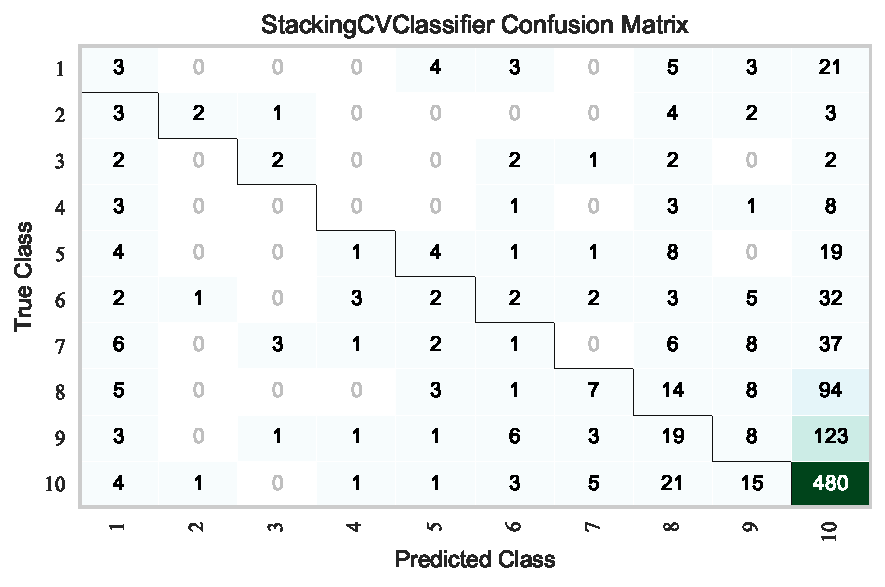
\includegraphics[scale=0.60]{[附件1]模型二混淆矩阵热力图.pdf}}
			\caption{模型二混淆矩阵热力图[语音业务-网络覆盖与信号强度]}\label{fig:SecondModelConfusionMatrix}
		\end{figure}

		观察该图,我们可以发现,该模型对于预测用户评分具有较好的效果,主对角线附近元素较多,说明模型预测正确的误差较小,预测得分与用户实际评分比较接近,可以较好预测用户评分。

		\item \textbf{分类报告}。分类报告图示可以直观得到模型各项参数,包括每一类别的精确率(Precision),召回率(Recall),F1分数值(F1-Score)。对于这三项值,其计算公式如下:
		\begin{itemize}
			\item {\heiti 精确率}
			\begin{equation}
				\mathrm{Precision} = \frac{TP}{TP+FP} \label{Precision}
			\end{equation}
			\item {\heiti 召回率}
			\begin{equation}
				\mathrm{Recall} = \frac{TP}{TP+FN} \label{Recall}
			\end{equation}
			\item {\heiti F1分数值} 
			\begin{equation}
				\mathrm{F}1 = \frac{2\times \mathrm{Precision}\times \mathrm{Recall}}{\mathrm{Precision}+\mathrm{Recall}}=\frac{TP}{TP+\frac{1}{2}\left(FP+FN\right)} \label{F1-Score}
			\end{equation}
		\end{itemize}
		根据上述\textcolor{blue}{\eqref{Precision}}、\textcolor{blue}{\eqref{Recall}}、\textcolor{blue}{\eqref{F1-Score}},我们可以计算出每一个模型对于每一类别的三项指标值,并绘制分类报告图,对于模型二的分类报告,见\textcolor{blue}{\cref{fig:SecondModelClassificationReport}}。
		\begin{figure}[htbp]
			\centerline{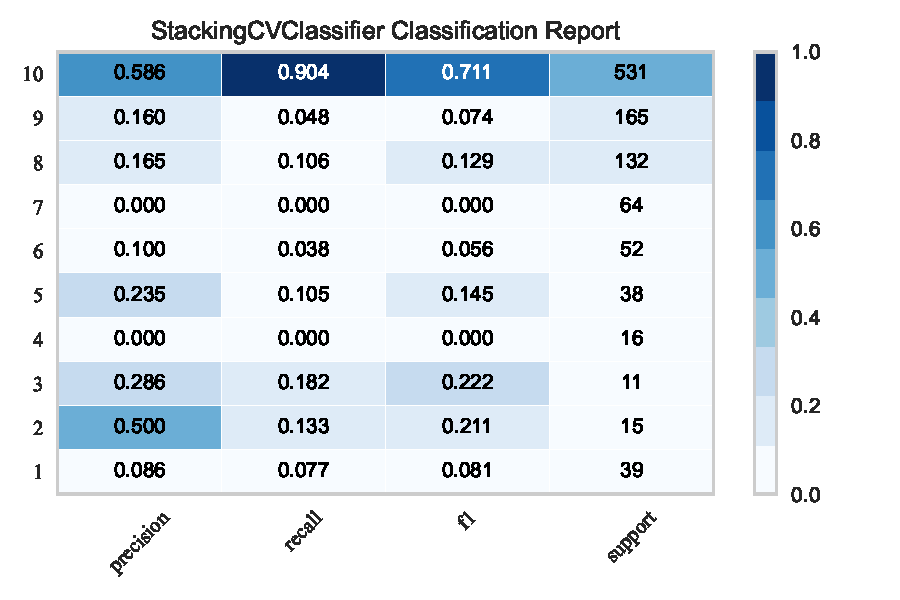
\includegraphics[scale=0.50]{[附件1]模型二分类报告.pdf}}
			\caption{模型二分类报告[语音业务-网络覆盖与信号强度]}\label{fig:SecondModelClassificationReport}
		\end{figure}

		对于模型的精确率、召回率,我们可以根据定义发现,这两项值显然较大,模型效果较好。同时根据定义,我们可以发现模型的精确率、召回率在理想情况下是相差较小的,我们可以根据图表结果验证,符合预期效果。对于模型的F1分数值,其为精确率与召回率的调和平均数,因此当精确率与召回率均有较好表现时,F1分数值会有较优秀表现。我们也可对\textcolor{blue}{\eqref{F1-Score}}进行一定变换,可以得到
		\begin{equation}
			\mathrm{F}1=\frac{2}{\frac{1}{\mathrm{Precision}}+\frac{1}{\mathrm{Recall}}} \label{ReacllNew}
		\end{equation}
		根据该式,我们可以得出上述结论。
		\item \textbf{ROC/AUC曲线}。在分析特征曲线及曲线下面积(Receiver Operating Characteristic/Area Under the Curve, ROC/AUC)图之前,我们需要了解模型的相关参数,定义如下:
		\begin{itemize}
			\item {\heiti 灵敏度}\textbf{(Sensitivity)}。灵敏度又被称为真阳性率,即$TP$率,定义为:
			\begin{equation}
				\mathrm{Sensitivity}=TPR=\frac{TP}{TP+FN} \label{Sensitivity}
			\end{equation}
			\item {\heiti 特异性}\textbf{(Specificity)}。特异性又被称为真阴性率,即$TN$率,定义为:
			\begin{equation}
				\mathrm{Specificity}=TNR=\frac{TN}{TN+FP} \label{Specificity}
			\end{equation}
			\item \textbf{1-Specificity}。称为假阳性率(False Positive Rate, $FPR$),定义为:
			\begin{equation}
				FPR=1-\mathrm{Specificity}=\frac{FP}{FP+TN} \label{FPR}
			\end{equation}
			\item \textbf{1-Sensitivity}。称为假阴性率(False Negative Rate, $FNR$),定义为:
			\begin{equation}
				FNR=1-\mathrm{Sensitivity}=\frac{FN}{FN+TP} \label{FNR}
			\end{equation}
		\end{itemize}
		$FPR$和$FNR$均对数据分布的变化不敏感\textcolor{blue}{\cite{procauc}},因此这两个指标可以用于在不平衡的数据上建立的模型效果的评价。
		
		对于ROC/AUC曲线,其以每一类别的$1-\mathrm{Specificity}$即$FPR$为横坐标,以$\mathrm{Sensitivity}$即$TPR$为纵坐标,其可体现出模型的灵敏度与特异性之间的关系与差异。因此,该图的理想点位于左上角,即$FPR=0$且$TPR=1$,换言之,当曲线越靠近左上角,模型效果就越优。从而,我们可以得到另一项指标,即曲线下面积(Area Under the Curve, AUC),由上述分析可知,AUC值越高,模型的整体效果也就越优。对于模型二的ROC/AUC曲线,见\textcolor{blue}{\cref{fig:SecondModelROCAUC}}。
		\begin{figure}[H]
			\centerline{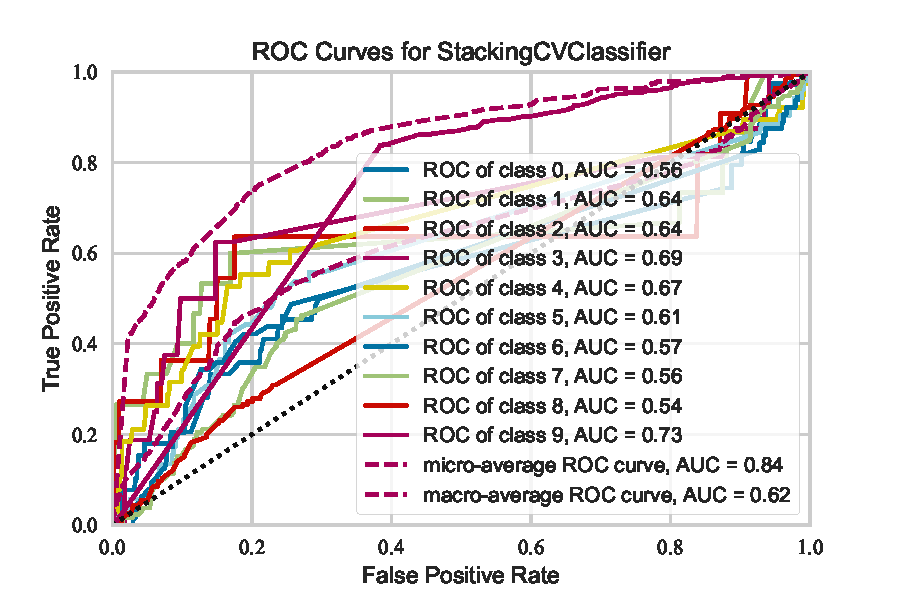
\includegraphics[scale=0.60]{[附件1]模型二ROCAUC.pdf}}
			\caption{模型二ROC/AUC曲线[语音业务-网络覆盖与信号强度]}\label{fig:SecondModelROCAUC}
		\end{figure}
		根据上图结果,我们可以发现,模型二预测用户对于“语音业务-语音通话整体满意度”的评分结果中,模型对各评分预测的$\mathrm{AUC}\geqslant0.50$,即以$y=x$为分界线。同时,我们可以发现“macro-average ROC curve”指标,其是通过Macro方法求得,在上文中我们提到,该数据样本的标签分类是严重不平衡的,该方法能够平等对待每一项分类,在此方法下,我们可以对于小样本类别的准确率有一定把握,其曲线下面积$\mathrm{AUC}=0.62$,位于分界线左上,预测效果良好;而对于“micro-average ROC curve”指标,其$\mathrm{AUC}=0.84$,这指的是利用Micro方法求得曲线,曲线下面积为0.84,曲线下面积较大,且曲线有向左上角最优点靠近的趋势,可以说明模型整体能力较优。
	\end{itemize}

	\section{模型的评价与推广}
	\subsection{模型的评价}
	\begin{itemize}
		\item \textbf{模型的优点}:
			\begin{enumerate}
				\item 对数据进行综合处理,层次清晰,模型具有一定解释性;
				\item 数据标准化,避免量纲不一造成的偏向学习影响的情况;
				\item 特征筛选,减少不重要性因素占比,减少数据维度,提升模型学习效率,一定程度上避免数据噪声,适当降低模型复杂度,使模型高效化,防止过拟合;
				\item 特征构造,由原数据构造出新数据特征,适当增多数据维度,防止欠拟合;
				\item 综合熵权法、灰色关联度分析及随机森林量化影响程度,避免局部最优;
				\item 对各模型进行参数调优,尽可能提高模型的多方面能力;
				\item 加入正则化方法,一定程度上也可防止过拟合;
				\item 交叉验证,更好地利用数据集,减少数据浪费,提高模型的泛化能力,验证模型的稳健性,防止过拟合情况的发生;
				\item 模型设置任意随机种子,在保证划分训练集及测试集的一般性、随机性的同时,确保可重复性的结果,方便后续处理;
				\item 通过主成分分析及随机森林进行特征选择,保证客观性;
				\item 多模型Stacking集成学习,更好地利用已有数据,多方面学习数据中内在联系,结合多个模型优良方面,避免陷入局部最优,对数据有更好的把控能力,提升模型的泛化能力、提高预测准确率、提高模型稳健性、鲁棒性,同时减小预测误差,且对异常值有一定识别能力。
			\end{enumerate}
		\item \textbf{模型的缺点}:
			\begin{enumerate}
				\item 模型对于小样本分类的识别能力较差,难以对这些用户进行深入分析;
				\item 模型对于预测主观性评分,难以提供完全一致的评分结果;
				\item Stacking在构造时,有一定复杂度,对基模型的要求较高;
				\item 对于部分评分,特征构造出的因素有一定局限性;
				\item 用户评分为主观性结果,本文大多模型选用客观性较强的模型进行解决,对数据利用有一定失真。
			\end{enumerate}
		\item \textbf{模型的改进}:
			\begin{enumerate}
				\item 在收集数据时,问卷设计需要更加合理化,多方面考虑其余未考虑到的影响因素对用户评分的影响;
				\item 在允许条件下获得更多训练样本;
				\item 对各模型可以选用非完全一致的特征,提升各模型的独特性,有目的地进行选择,减少学习的数据维度,加快模型收敛速度,使得模型学习高效化,结果准确化;
				\item 适当增加或减少数据维度,建立复杂度适中的模型;
				\item 对不平衡的多分类,可以采用“下采样”或“上采样”方法,使得分类平衡,但需要更多的数据集;
				\item 可适当增加基模型个数,并提高对基模型的筛选要求;
				\item 对主观性评分,可以建立主客观相结合的模型,从而优化模型各项指标。
			\end{enumerate}
	\end{itemize}
	\subsection{模型的推广}
	机器学习可利用现有的数据集进行有目的的训练,在此基础上预测分类标签下人为难以确定的结果,极大方便了当今对复杂数据的处理;多种机器学习相互结合,利用Stacking集成学习的方法,可以有效提高模型各方面能力,减少判断错误的情况。针对小部分样本的学习,需要更容易区分类别的特征进行学习,以及利用特征工程等方法进行解决。对于机器学习模型,我们可以作出其可视化图像,观察到模型的各项指标不易发现的问题,如欠拟合、过拟合等情况,我们可以依据模型效果评估可视化来对模型进行一定的调优。本文是以移动用户对业务的评分为基础,我们运用了多种机器学习的模型,再结合Stacking进行集成学习,可以发现模型的效果较优,对主观性评分模型有较好把控能力。利用该模型,可以根据用户对某些影响因素的情况,预测用户对于这项业务的满意程度,再结合相关描述性信息,有的放矢地解决用户遇到的问题,提升客户的满意程度,提升产品的服务质量,从而为业务创造更多价值。该模型在一定程度上虽有一定欠缺,但不仅仅可用于该领域的评分,也可用于其余领域,如用户对于某一产品的评价预测,根据用户评价,改善产品质量,提升经济效益,实现双赢。
	\newpage
	\section{非技术性报告}
	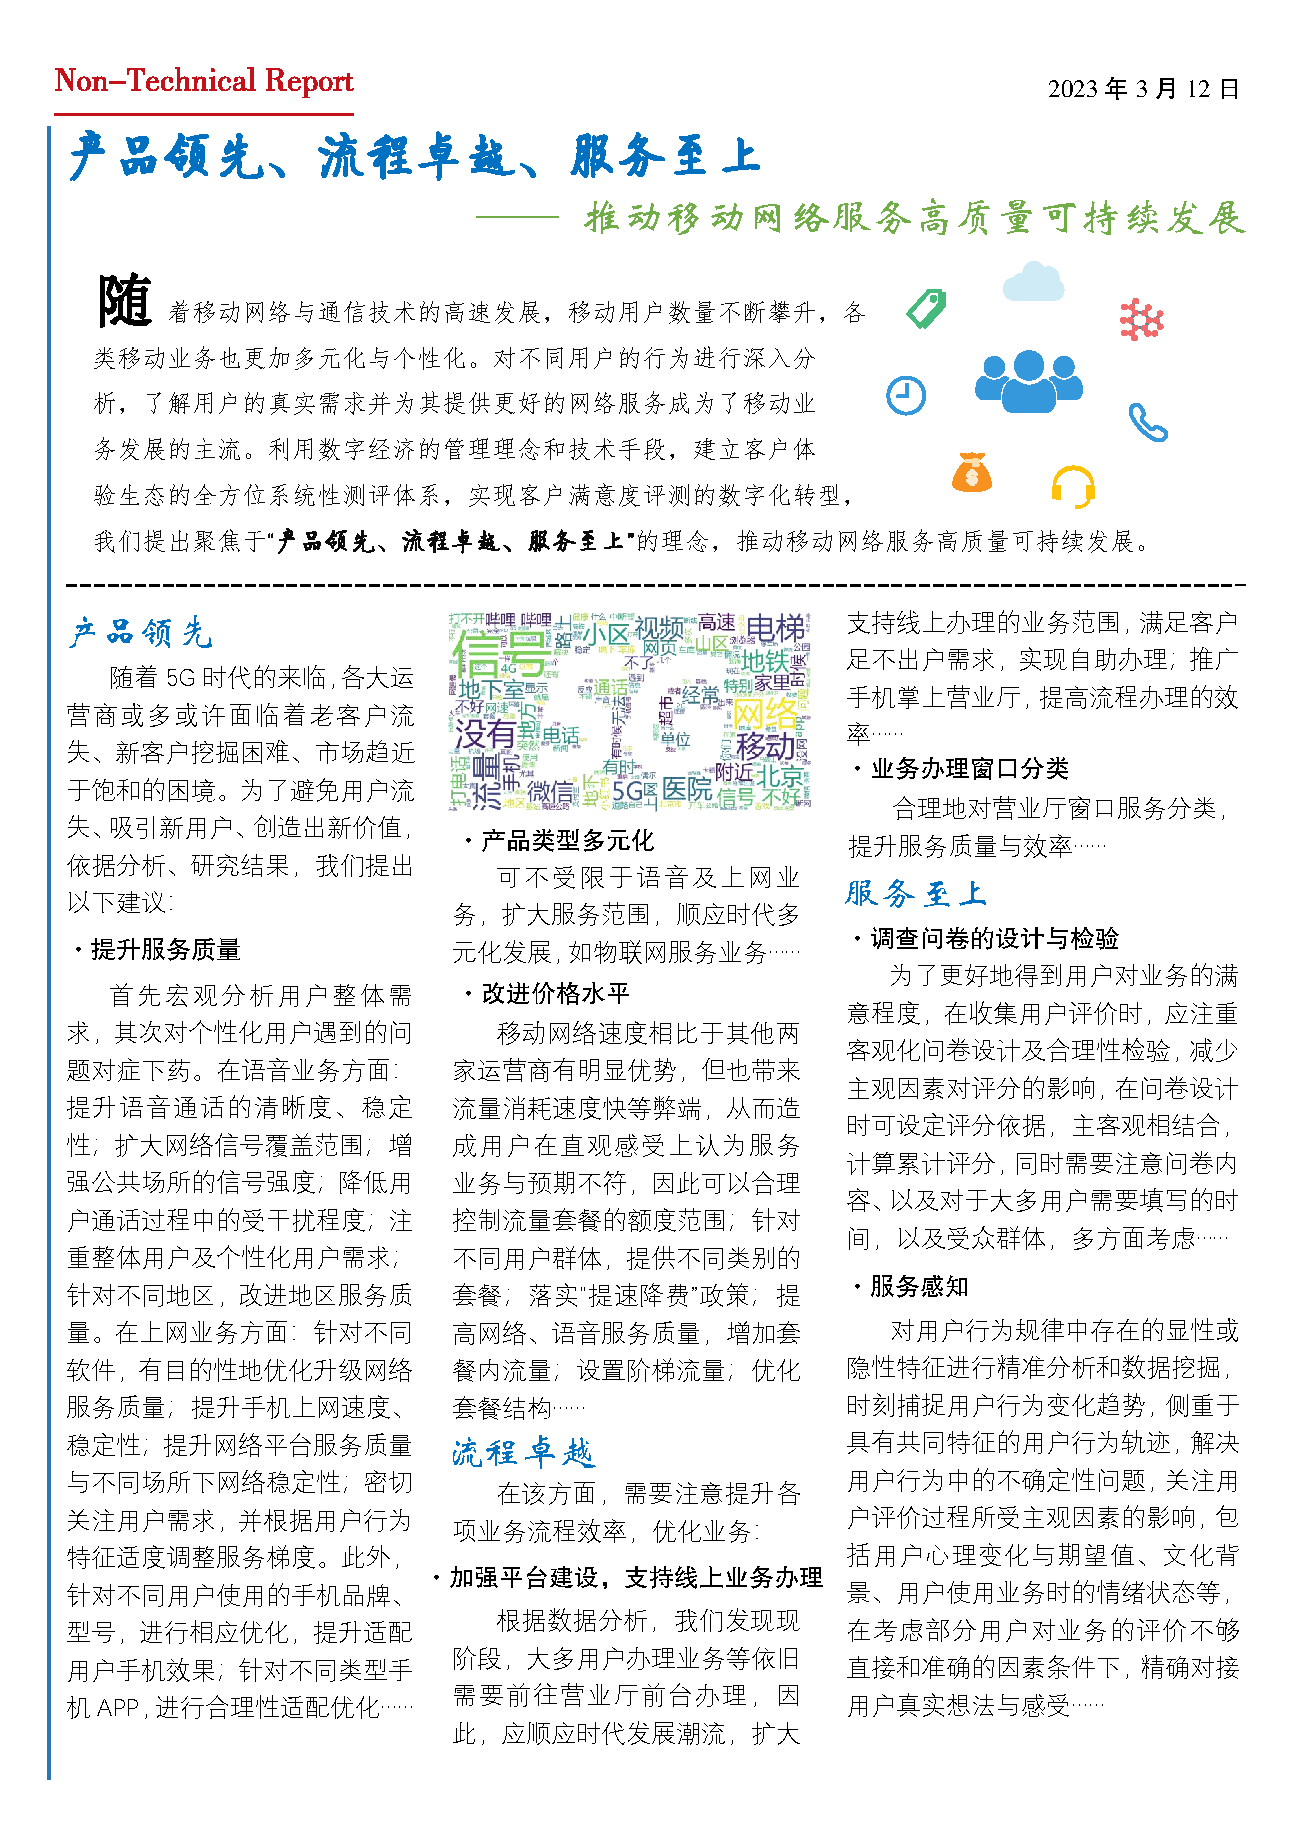
\includepdf[pages=-]{非技术性报告.pdf}

	\newpage
	\phantomsection
	\addcontentsline{toc}{section}{\textbf{参考文献}}
	\begin{spacing}{1.08}
	\begin{thebibliography}{99}
	\bibitem{pstandard}CSDN.【数据预处理】sklearn实现数据预处理(归一化、标准化)[EB/OL].
	
	\url{https://blog.csdn.net/weixin_44109827/article/details/124786873}.


	\bibitem{ppearson}王殿武,赵云斌,尚丽英,王凤刚,张震.皮尔逊相关系数算法在B油田优选化学防砂措施井的应用[J].精细与专用化学品,2022,30(07):26-28.DOI:10.19482/j.cn11-3237.2022.07.07.

	\bibitem{prf}饶雷,冉军,陶建权,胡号朋,吴沁,熊圣新.基于随机森林的海上风电机组发电机轴承异常状态监测方法[J].船舶工程,2022,44(S2):27-31.DOI:10.13788/j.cnki.cbgc.2022.S2.06.

	\bibitem{pxgboost1}陈振宇,刘金波,李晨,季晓慧,李大鹏,黄运豪,狄方春,高兴宇,徐立中.基于LSTM与XGBoost组合模型的超短期电力负荷预测[J].电网技术,2020,44(02):614-620.DOI:10.13335/j.1000-3673.pst.2019.1566.

	\bibitem{pxgboost2}杨贵军,徐雪,赵富强.基于XGBoost算法的用户评分预测模型及应用[J].数据分析与知识发现,2019,3(01):118-126.

	\bibitem{pxgboost3}Tianqi Chen and Carlos Guestrin. 2016. XGBoost: A Scalable Tree Boosting System. In Proceedings of the 22nd ACM SIGKDD International Conference on Knowledge Discovery and Data Mining (KDD '16). Association for Computing Machinery, New York, NY, USA, 785–794. \url{https://doi.org/10.1145/2939672.2939785}.

	\bibitem{pknn}张著英,黄玉龙,王翰虎.一个高效的KNN分类算法[J].计算机科学,2008(03):170-172.

	\bibitem{psvm}汪海燕,黎建辉,杨风雷.支持向量机理论及算法研究综述[J].计算机应用研究,2014,31(05):1281-1286.

	\bibitem{plightgbm}马晓君,沙靖岚,牛雪琪.基于LightGBM算法的P2P项目信用评级模型的设计及应用[J].数量经济技术经济研究,2018,35(05):144-160.DOI:10.13653/j.cnki.jqte.20180503.001.

	\bibitem{plr}唐敏,张宇浩,邓国强.高效的非交互式隐私保护逻辑回归模型[J/OL].计算机工程:1-11[2023-01-04].DOI:10.19678/j.issn.1000-3428.0065549.

	\bibitem{pstacking}史佳琪,张建华.基于多模型融合Stacking集成学习方式的负荷预测方法[J].中国电机工程学报,2019,39(14):4032-4042.DOI:10.13334/j.0258-8013.pcsee.181510.

	\end{thebibliography}
	\end{spacing}
	\newpage

	\phantomsection
	\addcontentsline{toc}{section}{\textbf{附\hspace{2pc}录}}

	% \appendix
	% \ctexset{section={format={\zihao{-4}\heiti\raggedright}}}
	\begin{center}
		\heiti\zihao{4} 附\hspace{2pc}录
	\end{center}

% \phantomsection
% \addcontentsline{toc}{subsection}{[A]图示}
% 	% \section*{[A]图表}
	\noindent{\heiti [A]图表}
	\begin{figure}[H]
		\centering
			\centering
			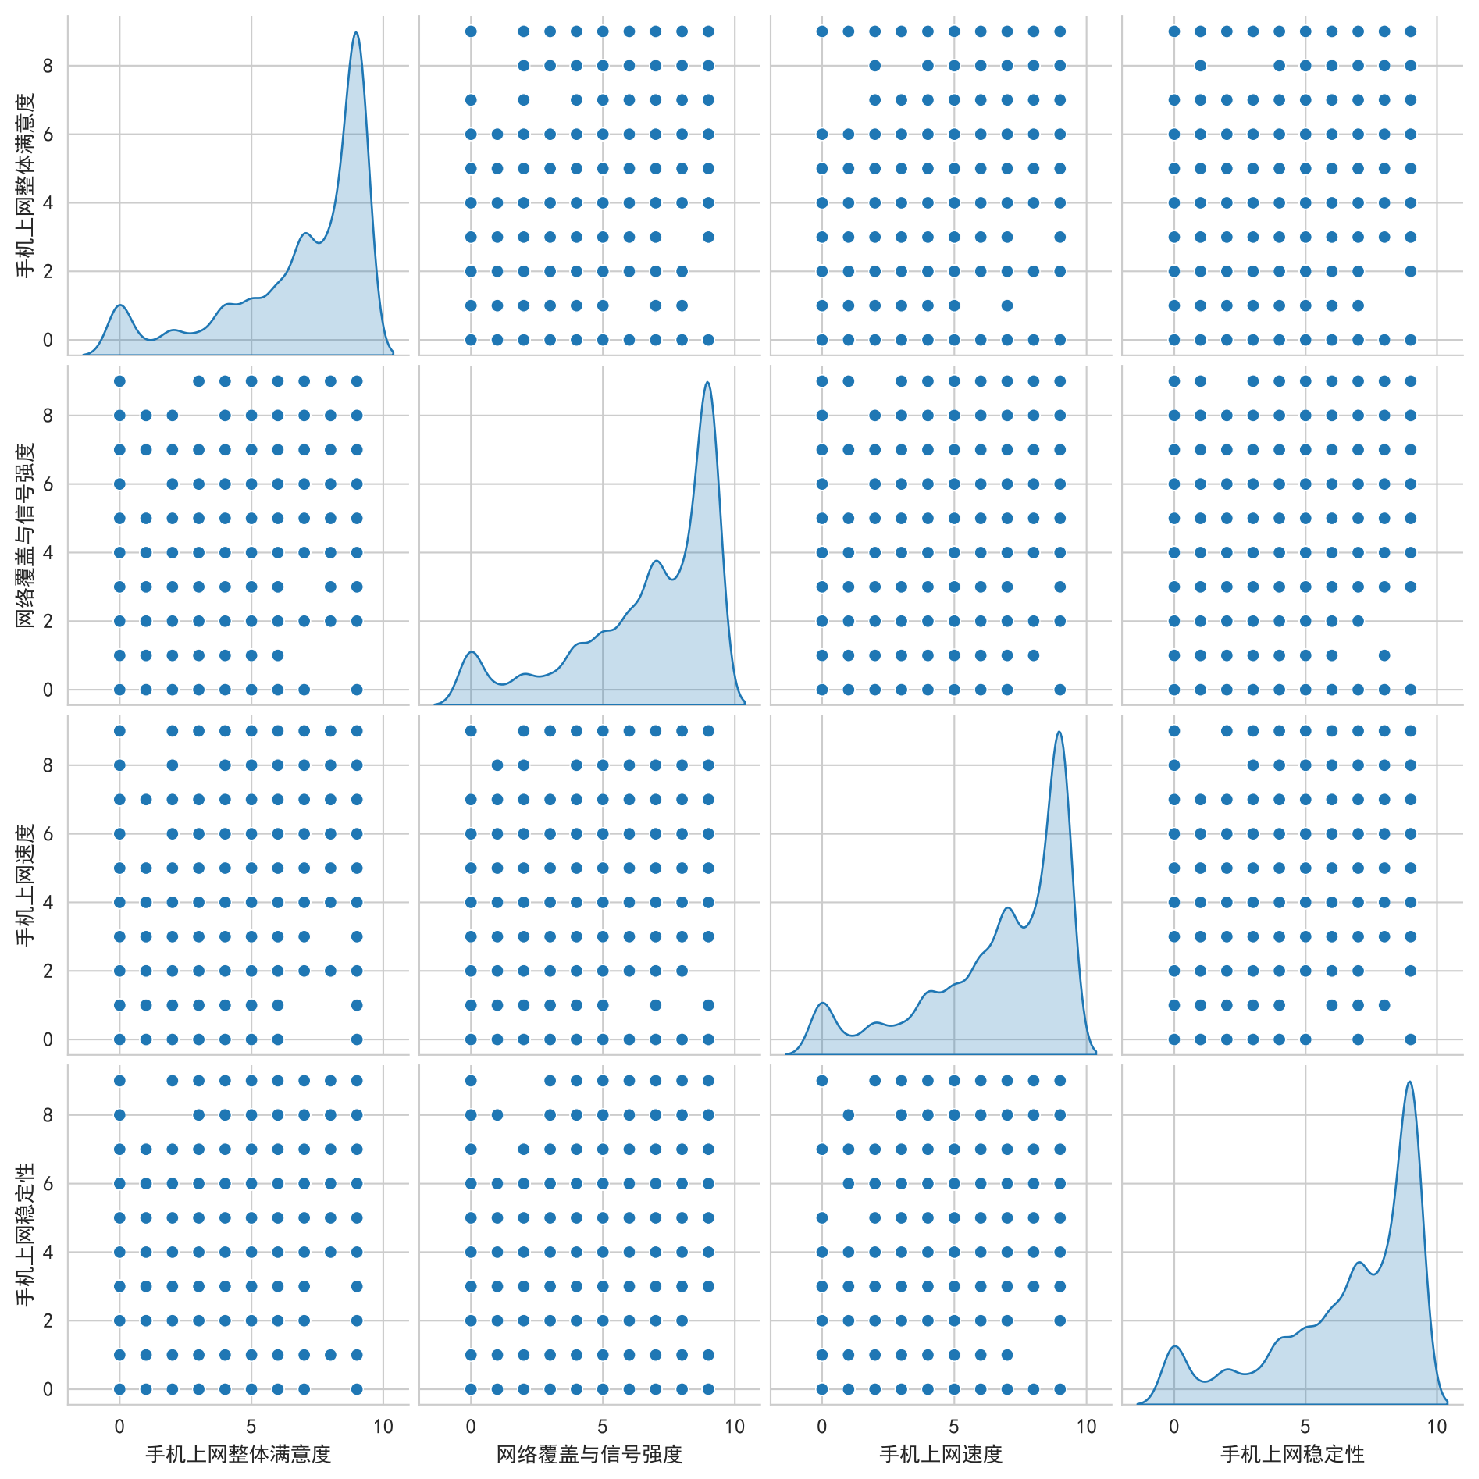
\includegraphics[width=0.66\linewidth]{[附件2][手机上网整体满意度、网络覆盖与信号强度、手机上网速度、手机上网稳定性]评分联合分布图_纯图版.pdf}
			\caption{上网业务用户四项评分联合分布图}
			\label{fig:上网业务联合分布图}
	\end{figure}
	\begin{figure}[H]
		\centering
		\begin{minipage}{0.48\linewidth}
			\centering
			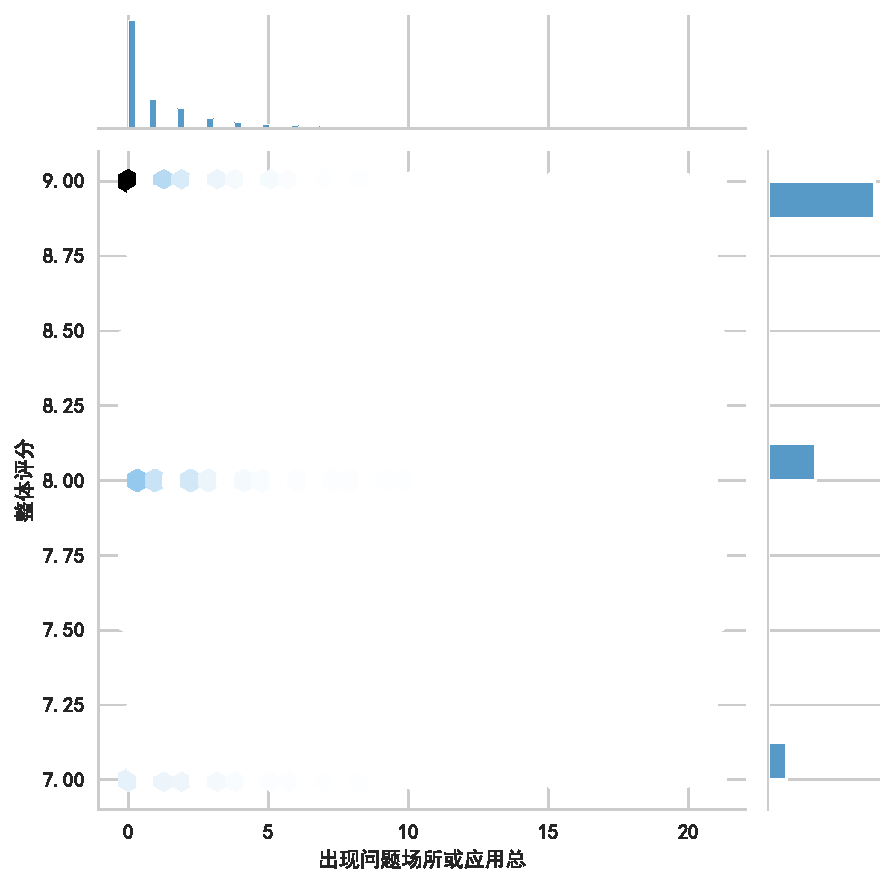
\includegraphics[width=0.70\linewidth]{[附件2]高分组出现问题场所或应用总分布.pdf}
			\caption{上网业务高分组问题及场所分布}
			\label{fig:上网业务高分组问题及场所分布}
		\end{minipage}
		%\qquad
		\begin{minipage}{0.48\linewidth}
			\centering
			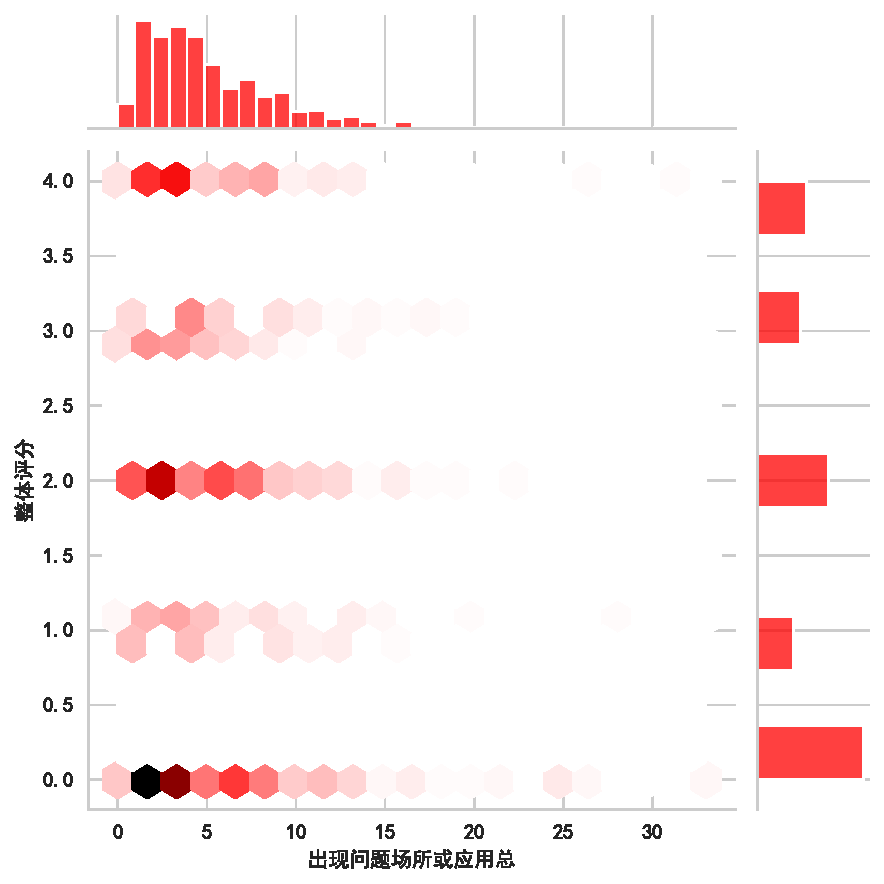
\includegraphics[width=0.70\linewidth]{[附件2]低分组出现问题场所或应用总分布.pdf}
			\caption{上网业务低分组问题及场所分布}
			\label{fig:上网业务低分组问题及场所分布}
		\end{minipage}
	\end{figure}
	\begin{figure}[H]
		\centering
		\begin{minipage}{0.48\linewidth}
			\centering
			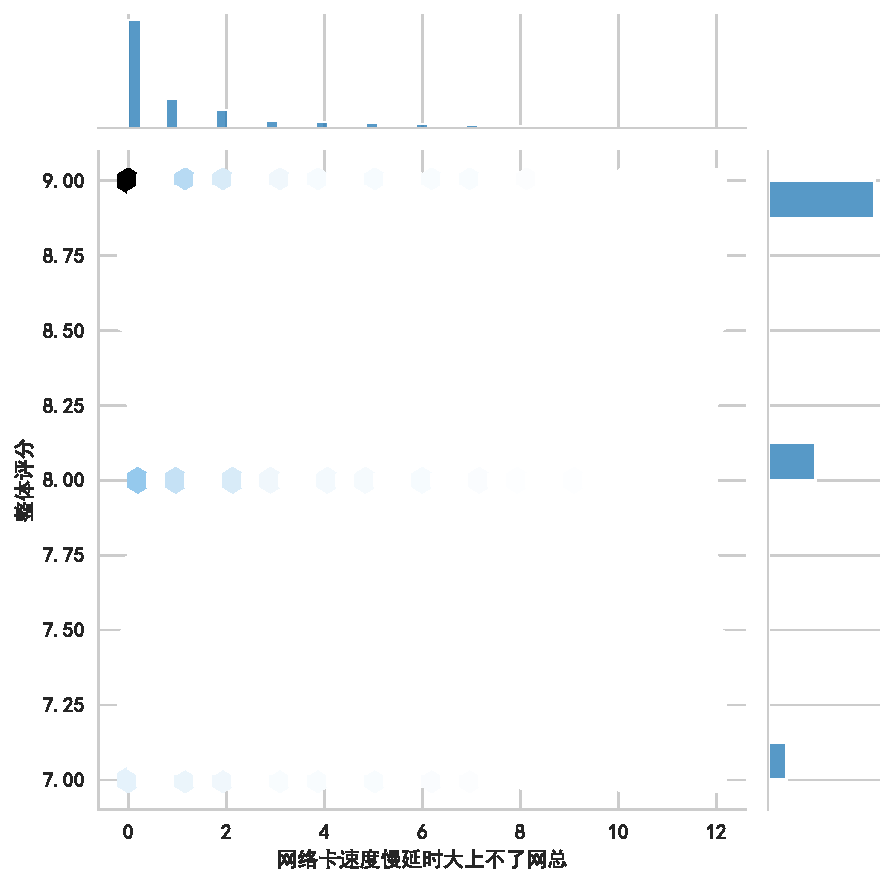
\includegraphics[width=0.70\linewidth]{[附件2]高分组网络卡速度慢延时大上不了网总分布.pdf}
			\caption{上网业务高分组网络不佳分布}
			\label{fig:上网业务高分组网络不佳分布}
		\end{minipage}
		%\qquad
		\begin{minipage}{0.48\linewidth}
			\centering
			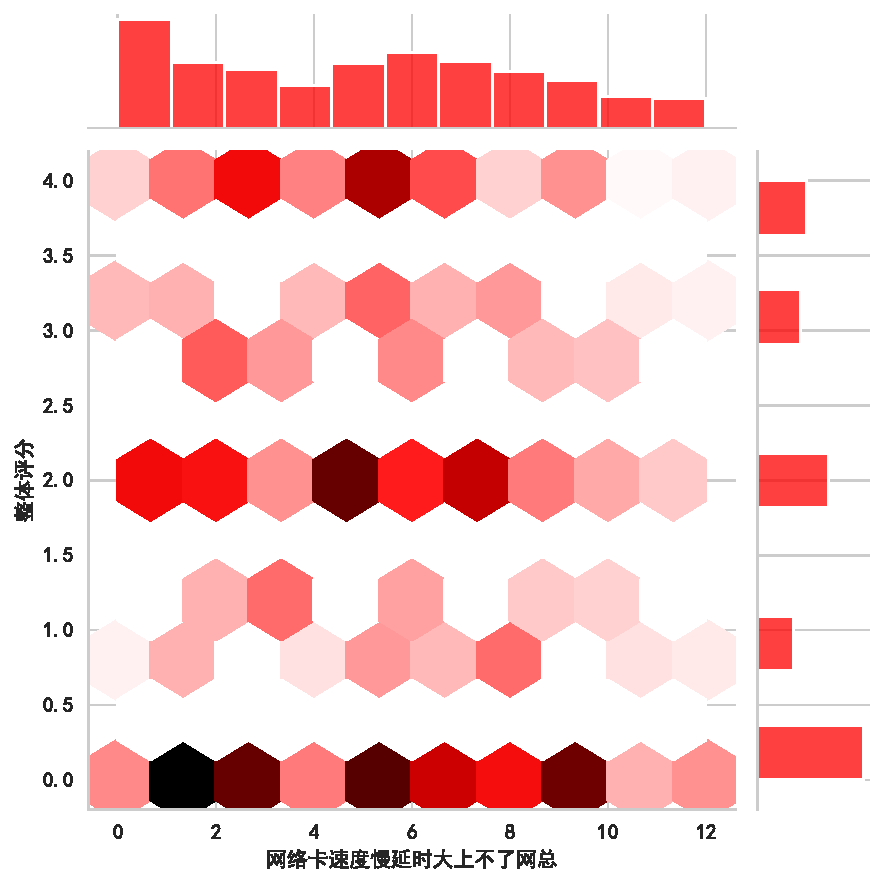
\includegraphics[width=0.70\linewidth]{[附件2]低分组网络卡速度慢延时大上不了网总分布.pdf}
			\caption{上网业务低分组网络不佳分布}
			\label{fig:上网业务低分组网络不佳分布}
		\end{minipage}
	\end{figure}
	\begin{figure}[H]
		\centering
		\begin{minipage}{0.48\linewidth}
			\centering
			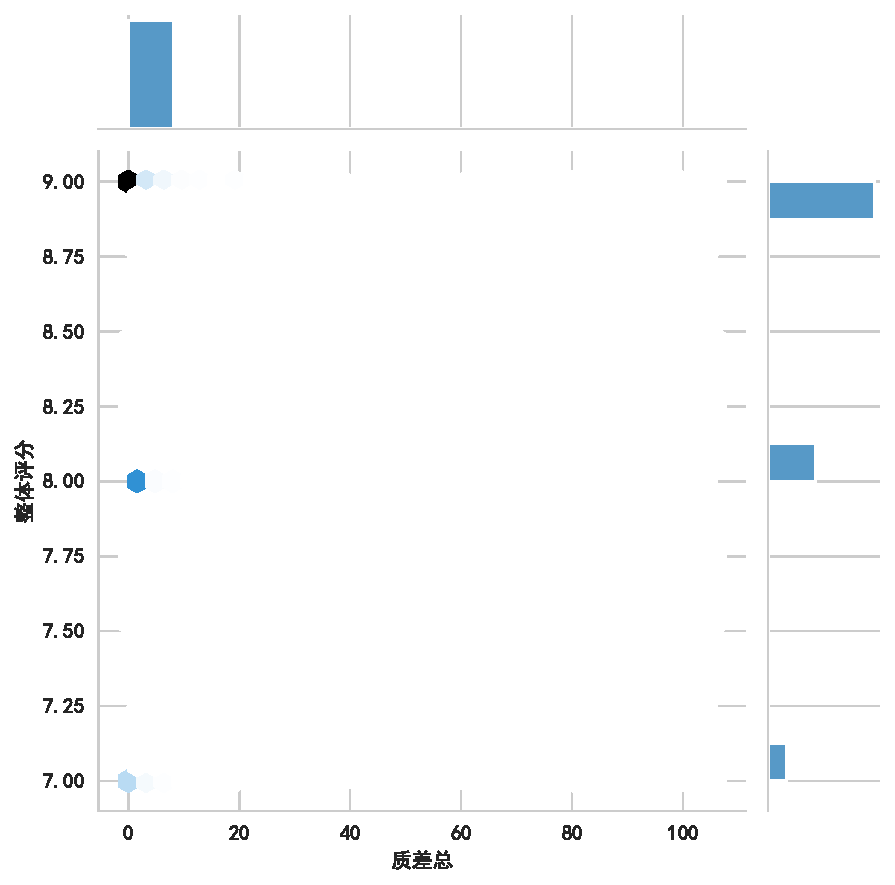
\includegraphics[width=0.70\linewidth]{[附件2]高分组质差总分布.pdf}
			\caption{上网业务高分组质差分布}
			\label{fig:上网业务高分组质差分布}
		\end{minipage}
		%\qquad
		\begin{minipage}{0.48\linewidth}
			\centering
			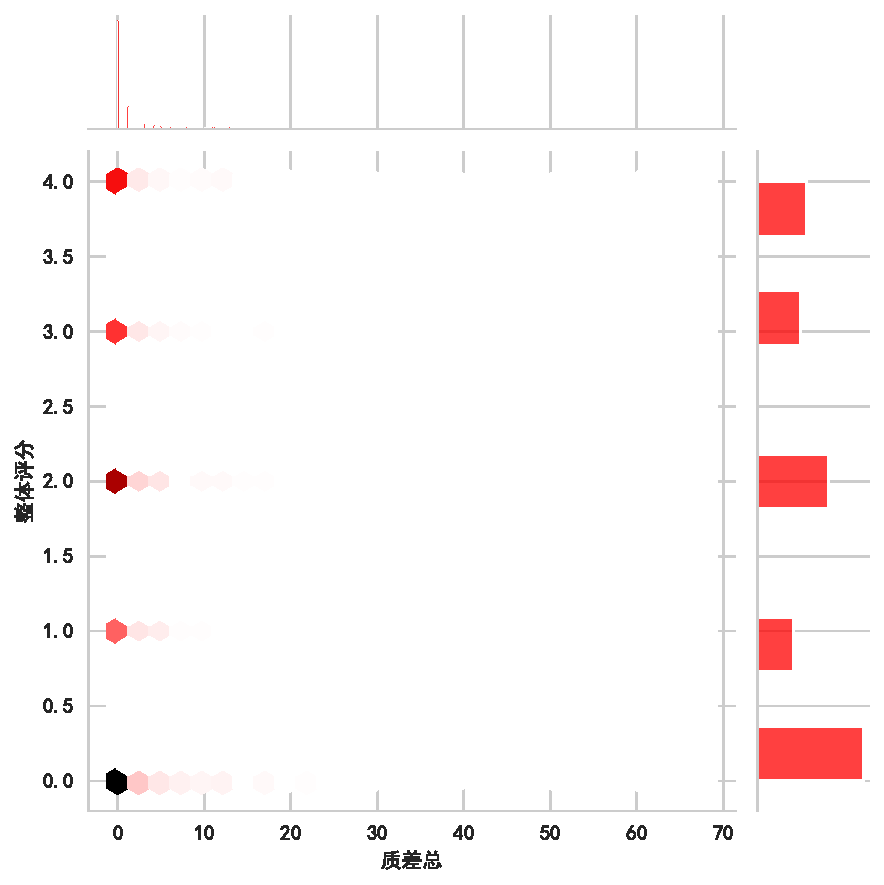
\includegraphics[width=0.70\linewidth]{[附件2]低分组质差总分布.pdf}
			\caption{上网业务低分组质差分布}
			\label{fig:上网业务低分组质差分布}
		\end{minipage}
	\end{figure}
	\begin{figure}[H]
		\centering
		\begin{minipage}{0.48\linewidth}
			\centering
			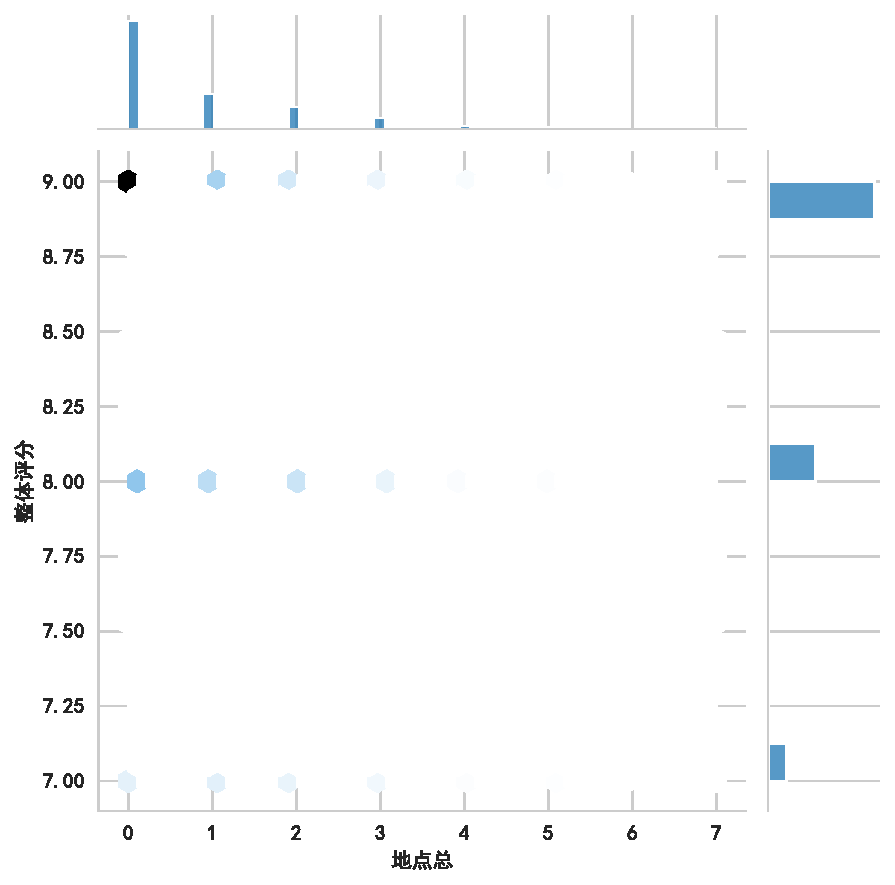
\includegraphics[width=0.70\linewidth]{[附件2]高分组地点总分布.pdf}
			\caption{上网业务高分组地点分布}
			\label{fig:上网业务高分组地点分布}
		\end{minipage}
		%\qquad
		\begin{minipage}{0.48\linewidth}
			\centering
			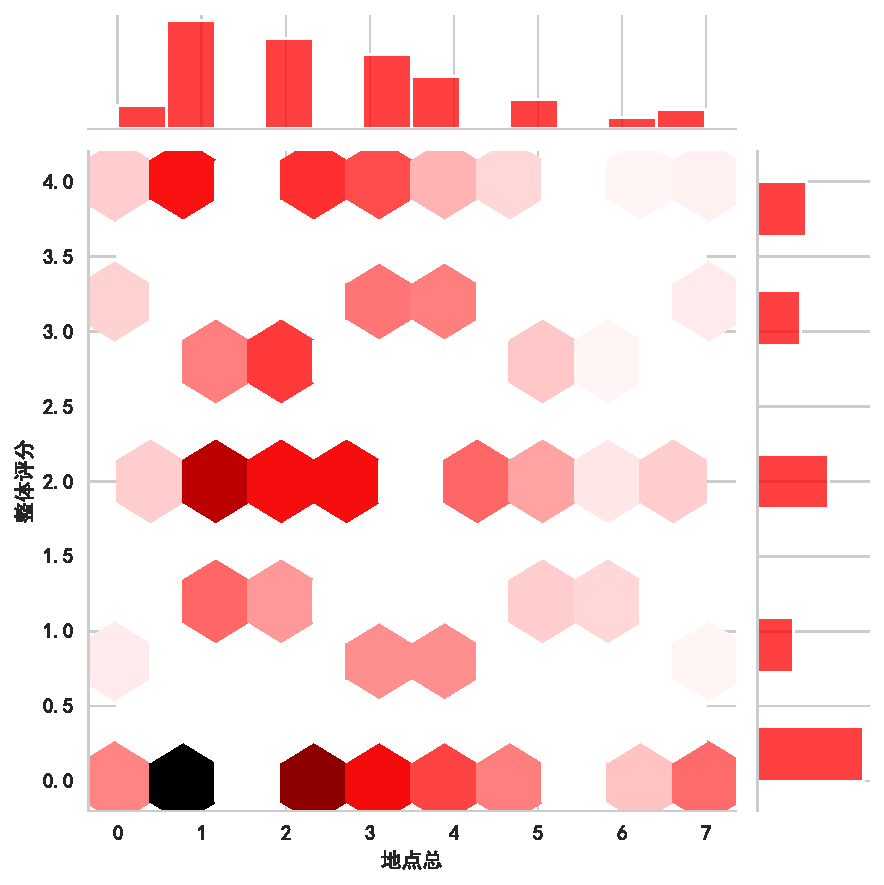
\includegraphics[width=0.70\linewidth]{[附件2]低分组地点总分布.pdf}
			\caption{上网业务低分组地点分布}
			\label{fig:上网业务低分组地点分布}
		\end{minipage}
	\end{figure}
	\begin{figure}[H]
		\centering
			\centering
			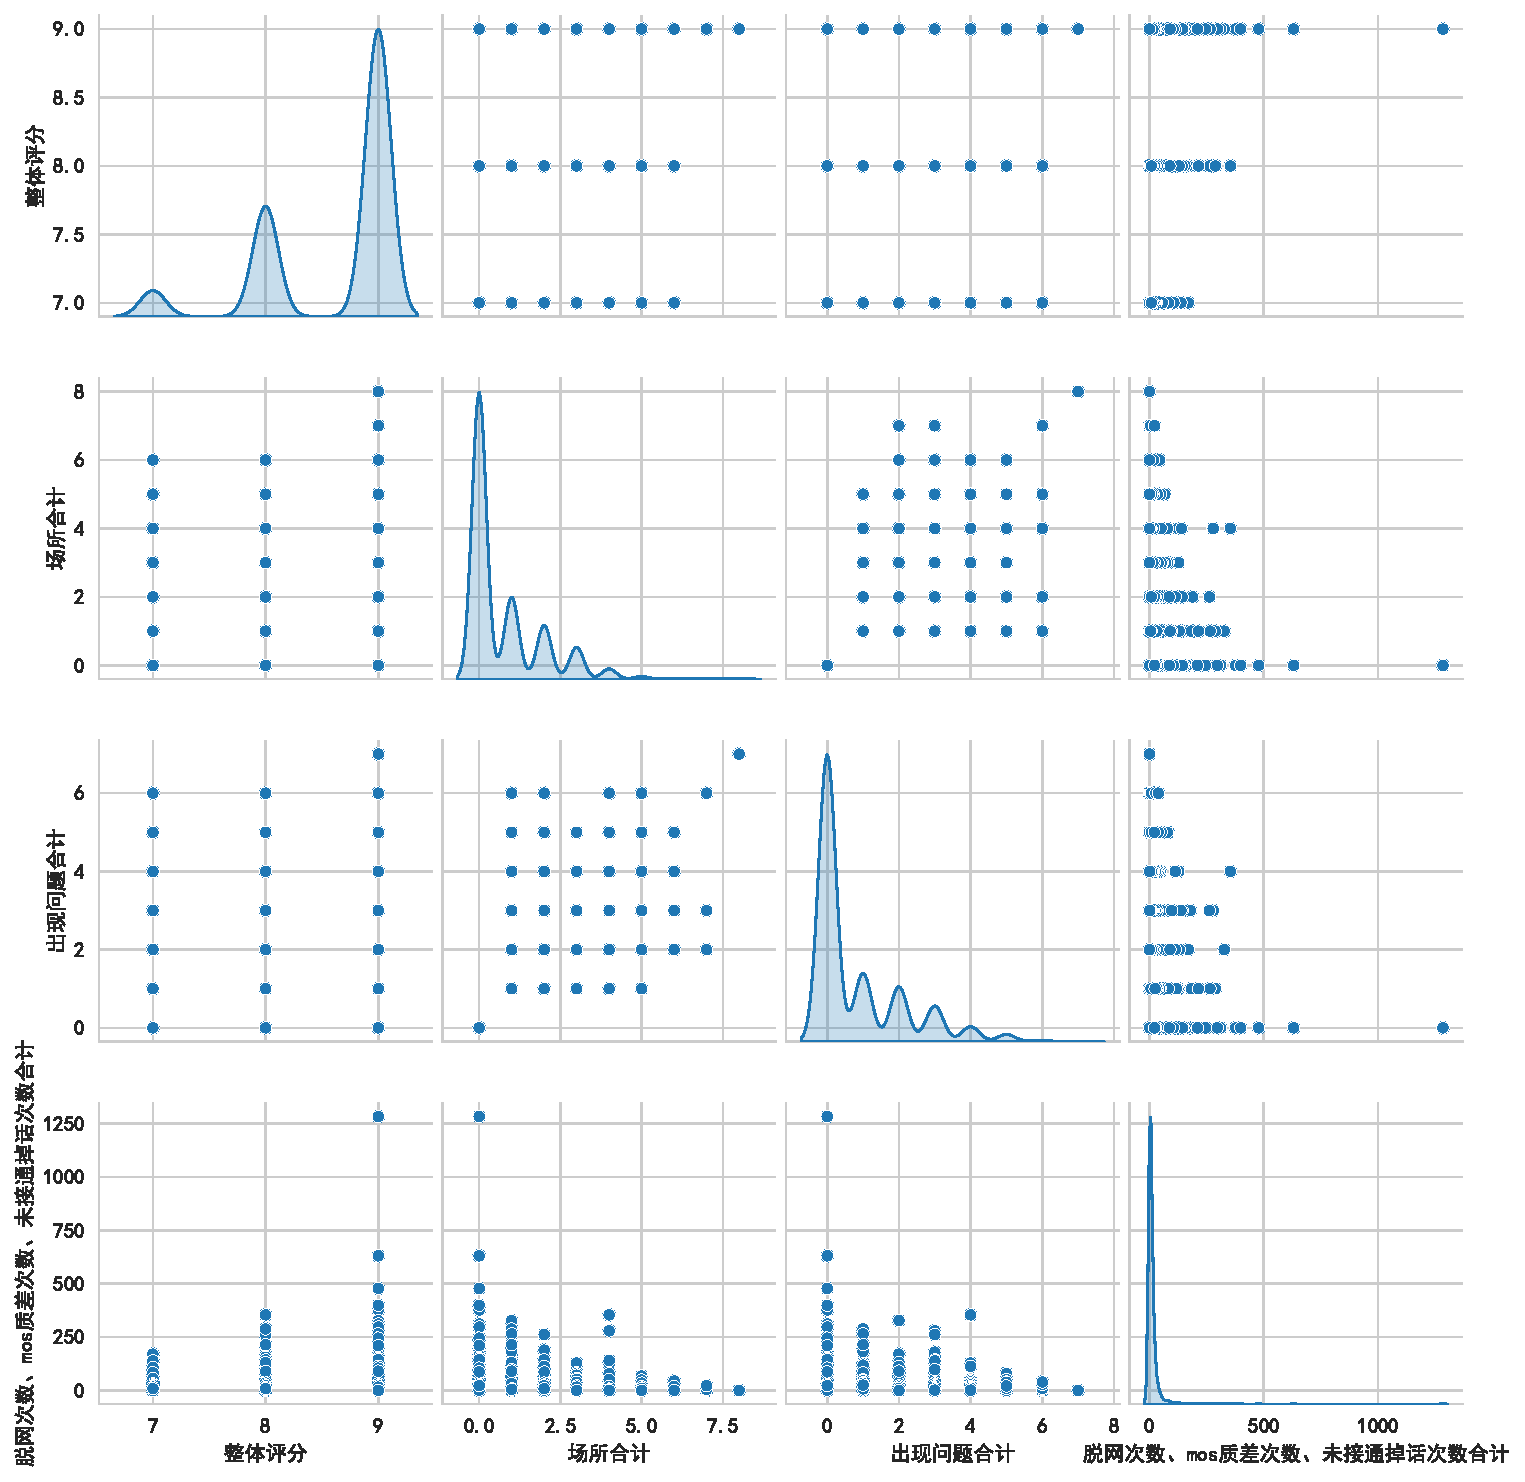
\includegraphics[width=0.66\linewidth]{[附件1]高分组[场所合计、出现问题合计、脱网次数、mos质差次数、未接通掉话次数合计]评分多变量联合分布图.pdf}
			\caption{语音业务高分组评分及特征多变量联合分布图}
			\label{fig:语音业务高分组评分及特征多变量联合分布图}
	\end{figure}	
	\begin{figure}[H]
		\centering
			\centering
			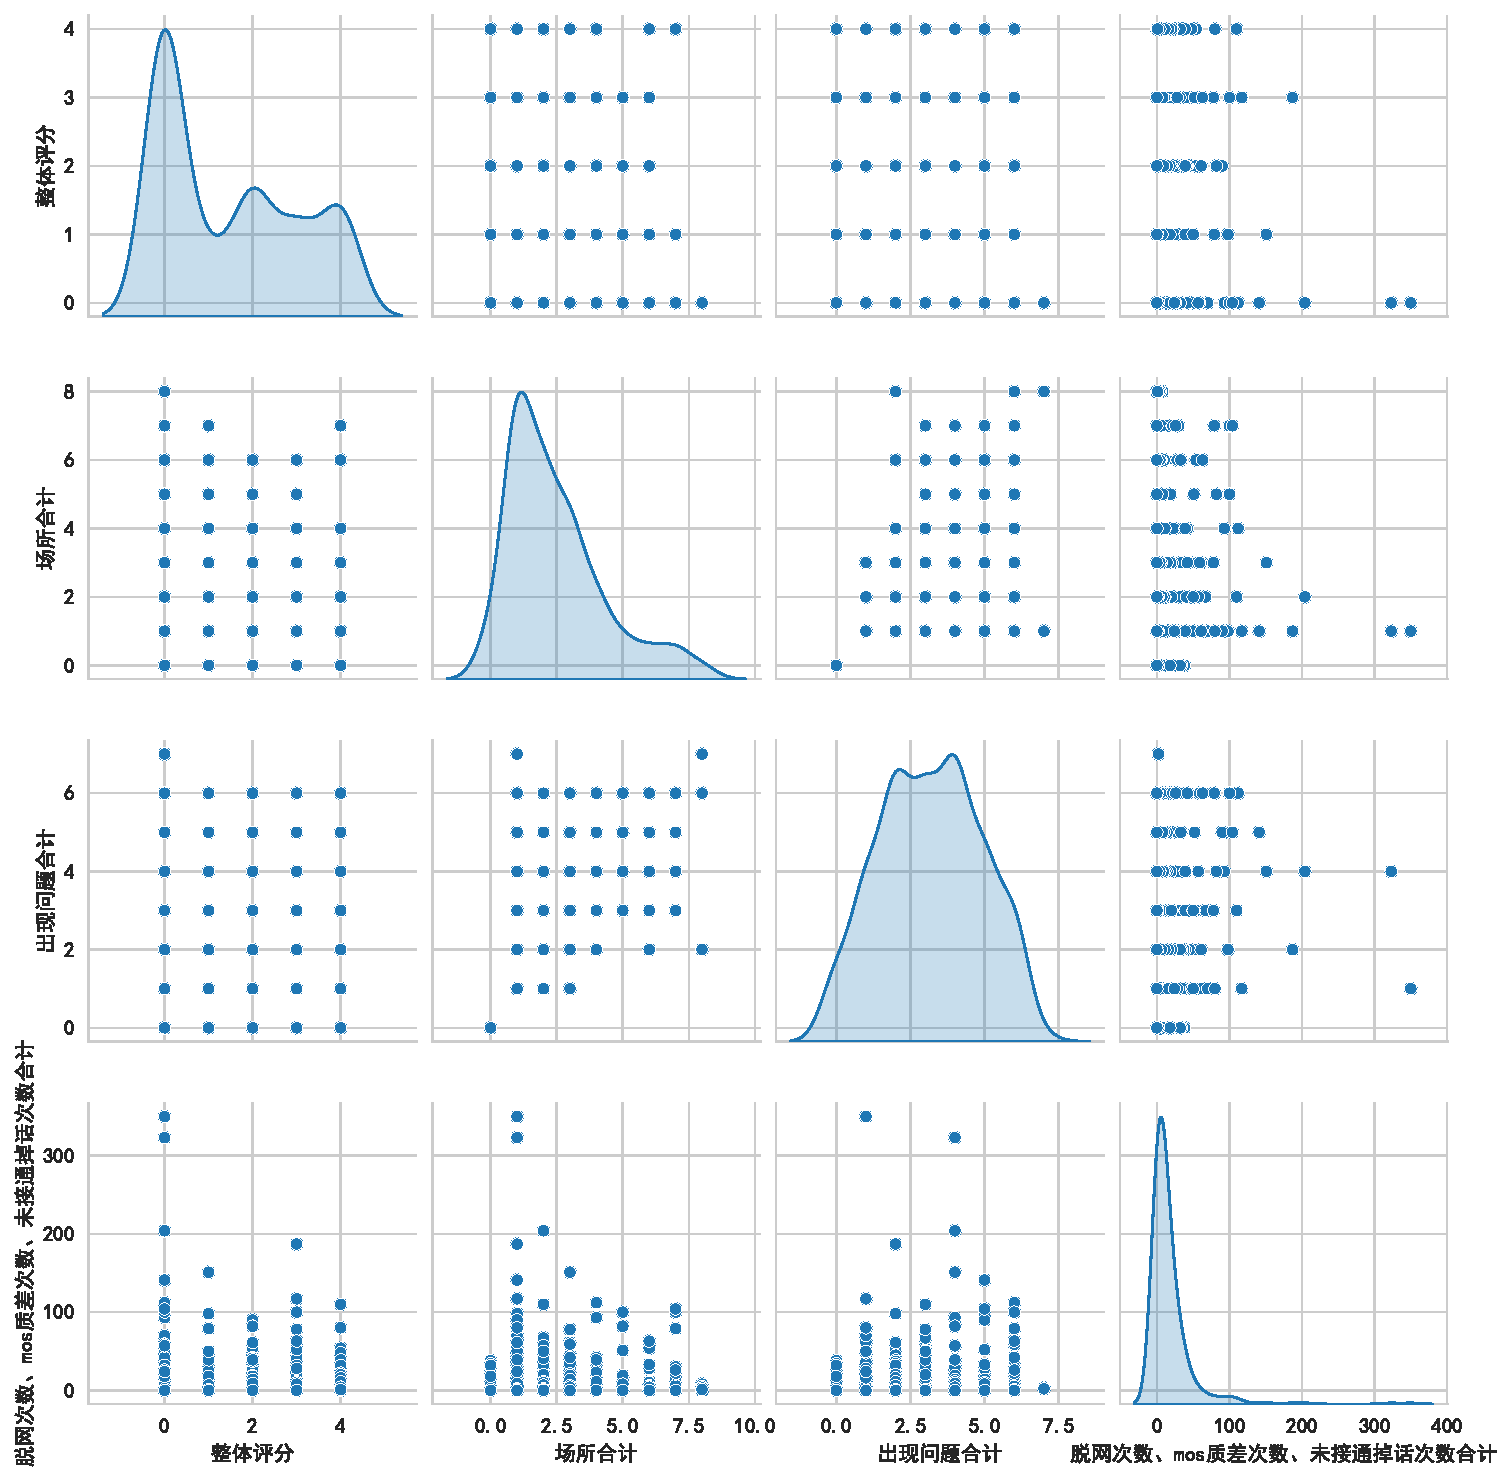
\includegraphics[width=0.66\linewidth]{[附件1]低分组[场所合计、出现问题合计、脱网次数、mos质差次数、未接通掉话次数合计]评分多变量联合分布图.pdf}
			\caption{语音业务低分组评分及特征多变量联合分布图}
			\label{fig:语音业务低分组评分及特征多变量联合分布图}
	\end{figure}
	\begin{figure}[H]
		\centering
			\centering
			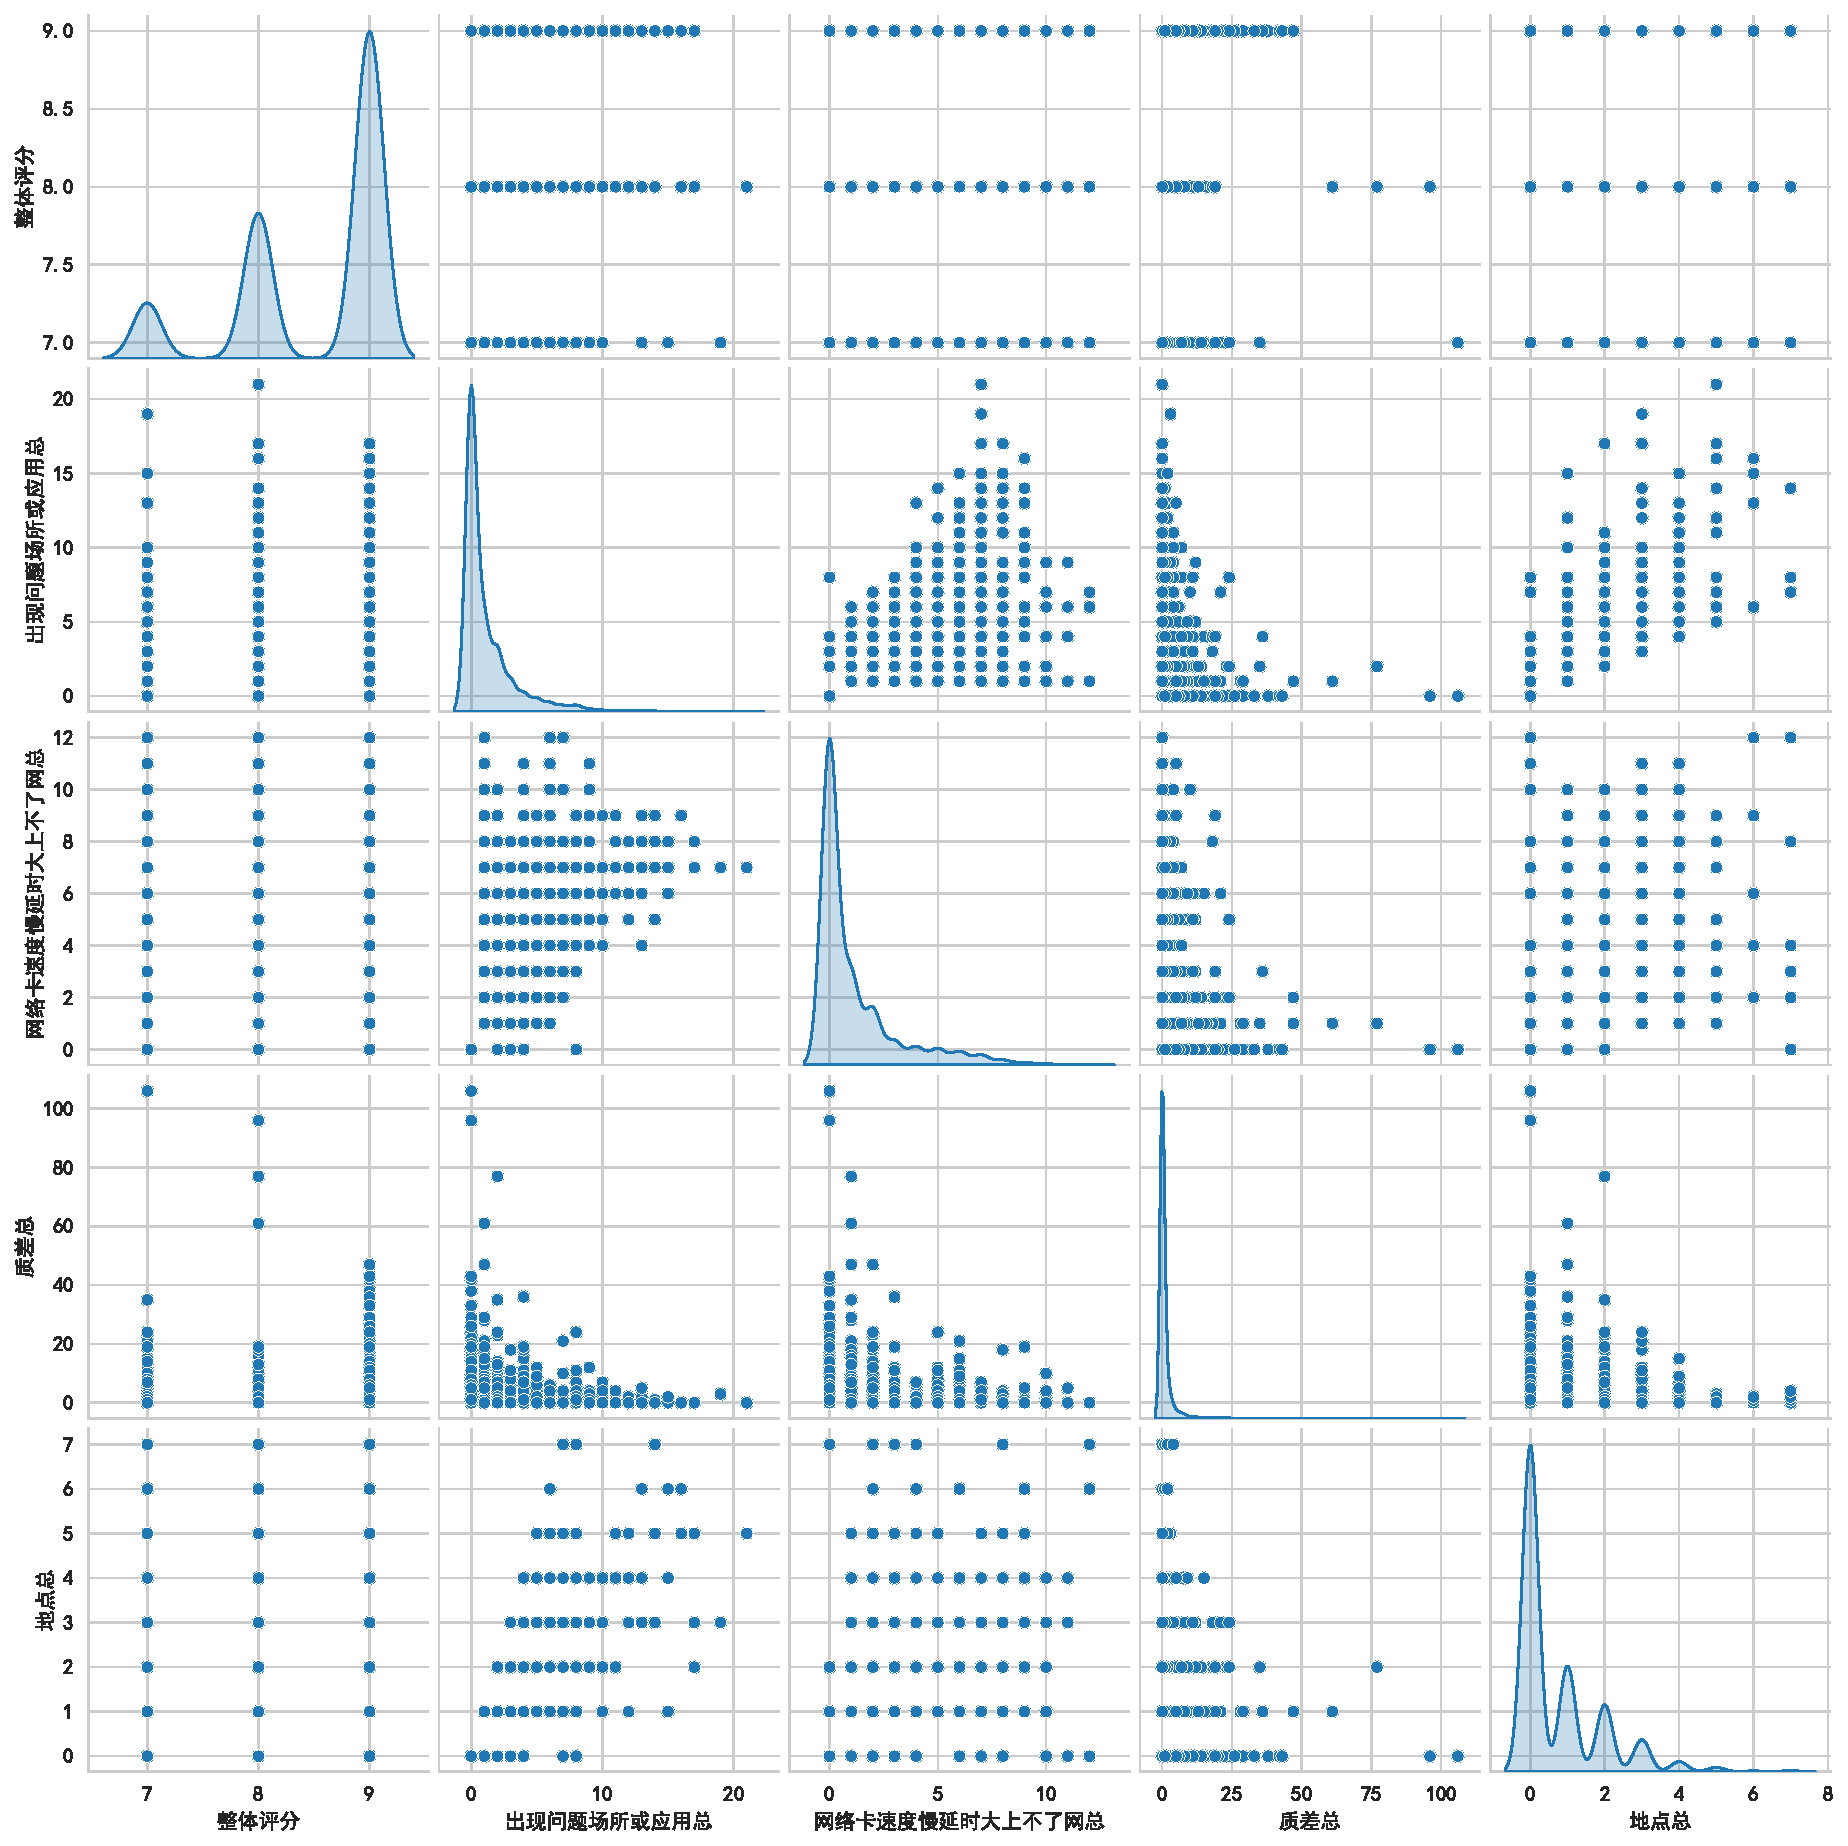
\includegraphics[width=0.66\linewidth]{[附件2]高分组[出现问题场所或应用总、网络卡速度慢延时大上不了网总、质差总、地点总]评分多变量联合分布图.pdf}
			\caption{上网业务高分组评分及特征多变量联合分布图}
			\label{fig:上网业务高分组评分及特征多变量联合分布图}
	\end{figure}	
	\begin{figure}[H]
		\centering
			\centering
			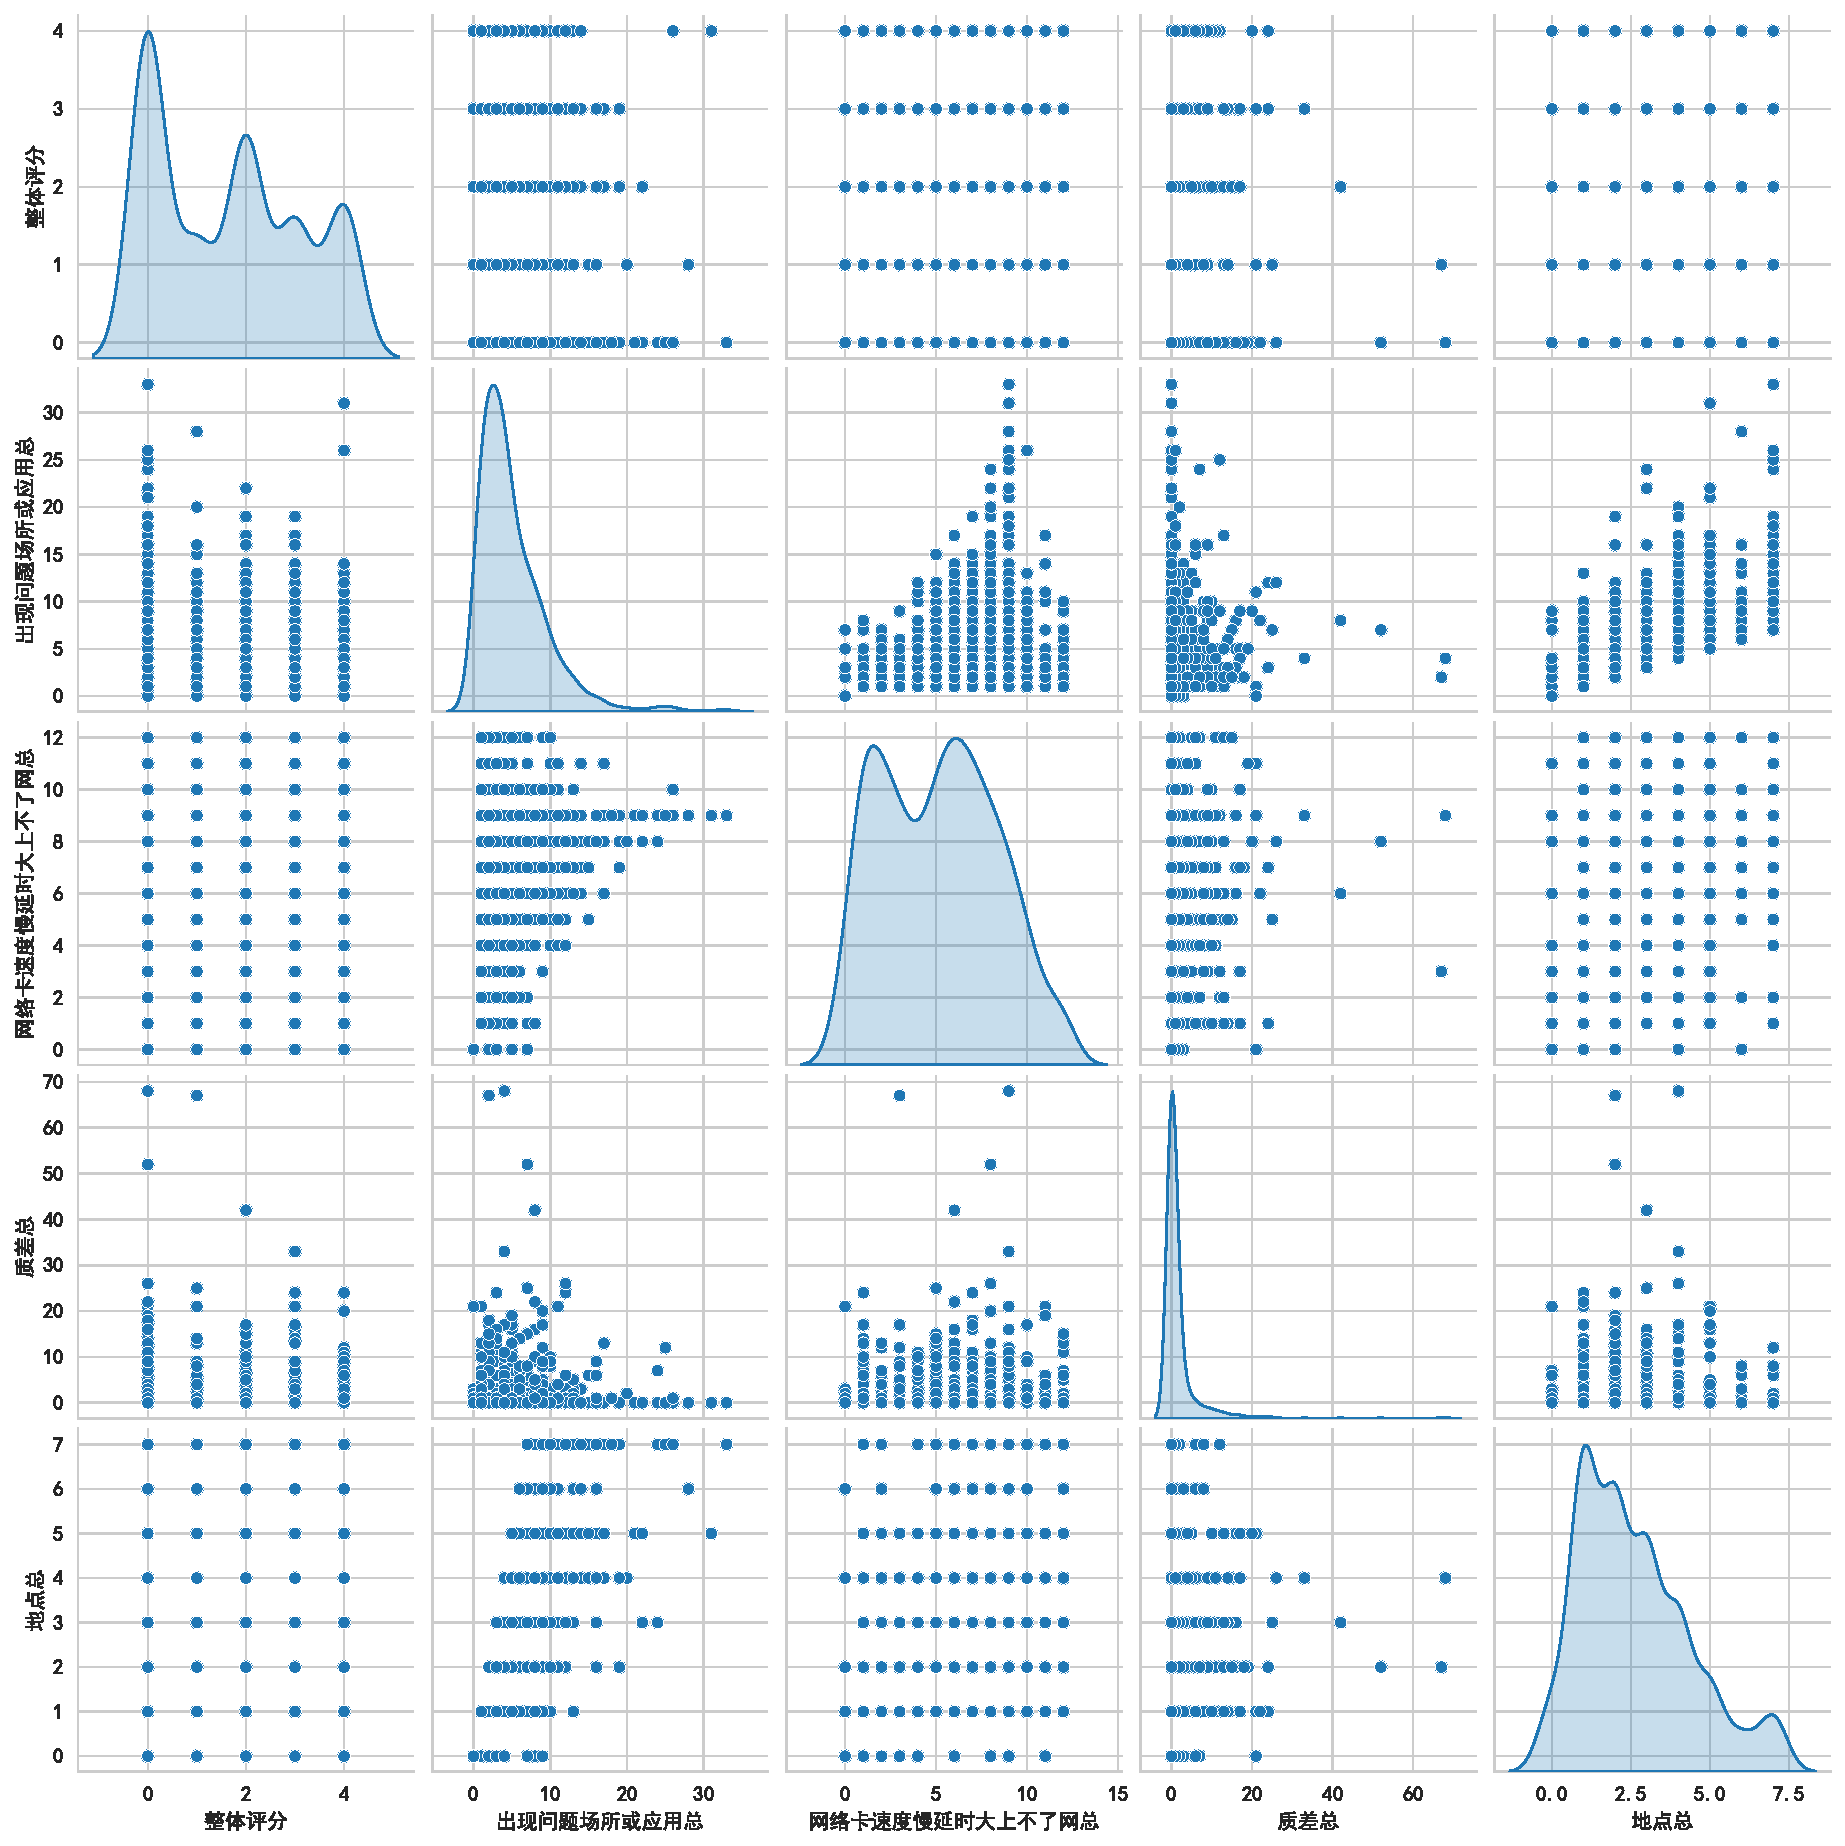
\includegraphics[width=0.66\linewidth]{[附件2]低分组[出现问题场所或应用总、网络卡速度慢延时大上不了网总、质差总、地点总]评分多变量联合分布图.pdf}
			\caption{上网业务低分组评分及特征多变量联合分布图}
			\label{fig:上网业务低分组评分及特征多变量联合分布图}
	\end{figure}
\newpage
% \phantomsection
% \addcontentsline{toc}{subsection}{[B]支撑文件列表}
% 	% \section*{[B]支撑文件列表}
	\noindent{\heiti [B]支撑文件列表}
	~\\

	支撑文件列表如下(列表中不包含原始数据集):
	% Table generated by Excel2LaTeX from sheet 'Sheet2'
	\begin{table}[htbp]
	\centering
	\scalebox{0.88}{
	  \begin{tabular}{cc}
	  \toprule
	  \textbf{文件(夹)名} & \textbf{描述} \\
	  \midrule
	  result.xlsx & 用户评分预测结果 \\
	  所有量化结果.xlsx & 问题一量化结果 \\
	  模型参数.xlsx & 各个模型评估参数以及模型选择依据 \\
	  语音业务词云.txt & 语音业务词云图文本内容 \\
	  上网业务词云.txt & 上网业务词云图文本内容 \\
	  语音业务数据分析.ipynb & 语音业务分析Jupyter文件 \\
	  上网业务数据分析.ipynb & 上网业务分析Jupyter文件 \\
	  语音业务数据分析.html & 语音业务分析运行结果 \\
	  上网业务数据分析.html & 上网业务分析运行结果 \\
	  bg.jpg & 词语底图 \\
	  figuresNightingaleRoseDiagramF.py & 原始数据用户评分南丁格尔玫瑰图程序 \\
	  figuresNightingaleRoseDiagramP.py & 预测数据用户评分南丁格尔玫瑰图程序 \\
	  figuresOne & 语音业务所有图示文件夹 \\
	  figuresTwo & 上网业务所有图示文件夹 \\
	  figuresNightingaleRoseDiagramF & 原始数据用户评分南丁格尔玫瑰图示(八项评分) \\
	  figuresNightingaleRoseDiagramP & 预测数据用户评分南丁格尔玫瑰图示(八项评分) \\
	  \bottomrule
	  \end{tabular}}
  	\end{table}
  
\newpage
% \phantomsection
% \addcontentsline{toc}{subsection}{[C]使用的软件、环境}
	% \section*{[C]使用的软件、环境}
	\noindent{\heiti [C]使用的软件、环境}
	~\\

	为解决该问题,我们所使用的主要软件有:
	\begin{itemize}
		\item TeX Live 2022
		\item Visual Studio Code 1.76.1
		\item WPS Office 2022冬季更新(13703)
		\item Python 3.10.4
		\item Pycharm Professional 2022.3
	\end{itemize}
	
	Python环境下所用使用到的库及其版本如下:
\begin{table}[htbp]
	\centering
	\setlength{\aboverulesep}{0pt}
	\setlength{\belowrulesep}{0pt}
	\scalebox{0.88}{
	  \begin{tabular}{cc||cc}
	  \toprule
	  \textbf{库} & \textbf{版本} & \textbf{库} & \textbf{版本} \\
	  \midrule
	  copy  & 内置库   & missingno & 0.5.1 \\
	  jieba & 0.42.1 & mlxtend & 0.20.2 \\
	  jupyter & 1.0.0 & numpy & 1.22.4+mkl \\
	  jupyter-client & 7.3.1 & openpyxl & 3.0.10 \\
	  jupyter-console & 6.4.3 & pandas & 1.4.2 \\
	  jupyter-contrib-core & 0.4.0 & pyecharts & 1.9.1 \\
	  jupyter-contrib-nbextensions & 0.5.1 & scikit-learn & 0.22.2.post1 \\
	  jupyter-core & 4.10.0 & seaborn & 0.11.2 \\
	  jupyter-highlight-selected-word & 0.2.0 & sklearn & 0.0  \\
	  jupyterlab-pygments & 0.2.2 & snapshot\_phantomjs & 0.0.3 \\
	  jupyterlab-widgets & 1.1.0 & warnings & 内置库 \\
	  jupyter-latex-envs & 1.4.6 & wordcloud & 1.8.1 \\
	  jupyter-nbextensions-configurator & 0.5.0 & xgboost & 1.6.1 \\
	  matplotlib & 3.5.2 & yellowbrick & 1.4 \\
	  \bottomrule
	  \end{tabular}}
\end{table}

\newpage
% \phantomsection
% \addcontentsline{toc}{subsection}{[D]问题解决源程序}
	% \section*{[D]问题解决源程序}
\noindent{\heiti [D]问题解决源程序}

\textbf{D.1 语音业务用户分析代码[针对附件1]}
\begin{python}
#!/usr/bin/env python
# coding: utf-8

# # 语音业务 用户行为分析

# ## 导入库

# In[1]:


import pandas as pd
import seaborn as sns


# ## 数据预处理

# In[2]:


dataOne=pd.read_excel("附件1语音业务用户满意度数据.xlsx",sheet_name='Sheet1')
dataThree=pd.read_excel("附件3语音业务用户满意度预测数据.xlsx",sheet_name='语音')


# In[3]:


dataOneColumnsList=list(dataOne.columns)
dataThreeColumnsList=list(dataThree.columns)


# In[4]:


dataOneColumnsList


# In[5]:


dataThreeColumnsList


# In[6]:


set(dataOneColumnsList)&set(dataThreeColumnsList)


# In[7]:


dataOne['资费投诉']=dataOne.loc[:, ['家宽投诉','资费投诉']].apply(lambda x1:x1.sum(), axis=1)
dataOne.drop(['家宽投诉'], axis=1, inplace=True)
dataOne.rename(columns={'资费投诉':'是否投诉'}, inplace=True)
dataOne


# In[8]:


dataOneColumnsList=list(dataOne.columns)
dataOneColumnsList


# In[9]:


dataThreeColumnsList=list(dataThree.columns)
dataThreeColumnsList


# In[10]:


set(dataOneColumnsList)-set(dataThreeColumnsList)


# In[11]:


dataOne.drop(['用户id',
              '用户描述',
              '用户描述.1',
              '重定向次数',
              '重定向驻留时长',
              '语音方式',
              '是否去过营业厅',
              'ARPU(家庭宽带)',
              '是否实名登记用户',
              '当月欠费金额',
              '前第3个月欠费金额',
              '终端品牌类型'], axis=1, inplace=True)
dataOne


# In[12]:


dataOne.info()


# In[13]:


dataOne.isnull().sum()


# In[14]:


dataOne['外省流量占比']=dataOne['外省流量占比'].fillna(0)
dataOne["是否关怀用户"]=dataOne["是否关怀用户"].fillna(0)
dataOne["外省流量占比"]=dataOne["外省流量占比"].astype(str).replace('%','')
dataOne["外省语音占比"]=dataOne["外省语音占比"].astype(str).replace('%','')
dataOne


# In[15]:


dataOne.replace({"是否遇到过网络问题":{2:0},
                 "居民小区":{-1:0},
                 "办公室":{-1:0,2:1},
                 "高校":{-1:0,3:1},
                 "商业街":{-1:0,4:1},
                 "地铁":{-1:0,5:1},
                 "农村":{-1:0,6:1},
                 "高铁":{-1:0,7:1},
                 "其他,请注明":{-1:0,98:1},
                 "手机没有信号":{-1:0},
                 "有信号无法拨通":{-1:0,2:1},
                 "通话过程中突然中断":{-1:0,3:1},
                 "通话中有杂音、听不清、断断续续":{-1:0,4:1},
                 "串线":{-1:0,5:1},
                 "通话过程中一方听不见":{-1:0,6:1},
                 "其他,请注明.1":{-1:0,98:1},
                 "是否关怀用户":{'是':1},
                 "是否4G网络客户(本地剔除物联网)":{'是':1,"否":0},
                 "是否5G网络客户":{'是':1,"否":0},
                 "客户星级标识":{'未评级':0,'准星':1,'一星':2,'二星':3,'三星':4,'银卡':5,'金卡':6,'白金卡':7,'钻石卡':8}
                 }, inplace=True)
dataOne


# In[16]:


dataOne.isnull().sum()


# In[17]:


dataOneMiss=dataOne.isnull()
dataOne[dataOneMiss.any(axis=1)==True]


# In[18]:


dataOne.dropna(inplace=True)
dataOne=dataOne.reset_index(drop=True)
dataOne


# In[19]:


dataOne.dtypes


# In[20]:


dataOne['外省语音占比'] = dataOne['外省语音占比'].astype('float64')
dataOne['外省流量占比'] = dataOne['外省流量占比'].astype('float64')
dataOne['是否4G网络客户(本地剔除物联网)'] = dataOne['是否4G网络客户(本地剔除物联网)'].astype('int64')
dataOne['4\\5G用户'] = dataOne['4\\5G用户'].astype(str)
dataOne['终端品牌'] = dataOne['终端品牌'].astype(str)
dataOne


# In[21]:


import sklearn.preprocessing as sp
le=sp.LabelEncoder()

OverallSatisfactionVoiceCalls=le.fit_transform(dataOne["语音通话整体满意度"])
NetworkCoverageSignalStrength=le.fit_transform(dataOne["网络覆盖与信号强度"])
VoiceCallDefinition=le.fit_transform(dataOne["语音通话清晰度"])
VoiceCallStability=le.fit_transform(dataOne["语音通话稳定性"])

FourFiveUser=le.fit_transform(dataOne["4\\5G用户"])
TerminalBrand=le.fit_transform(dataOne["终端品牌"])

dataOne["语音通话整体满意度"]=pd.DataFrame(OverallSatisfactionVoiceCalls)
dataOne["网络覆盖与信号强度"]=pd.DataFrame(NetworkCoverageSignalStrength)
dataOne["语音通话清晰度"]=pd.DataFrame(VoiceCallDefinition)
dataOne["语音通话稳定性"]=pd.DataFrame(VoiceCallStability)

dataOne["4\\5G用户"]=pd.DataFrame(FourFiveUser)
dataOne["终端品牌"]=pd.DataFrame(TerminalBrand)
dataOne


# In[22]:


def complain(x):
    if x!=0:
        return 1
    else:
        return 0


for i in range(len(dataOne)):
    dataOne.loc[i, '是否投诉']=complain(dataOne.loc[i, '是否投诉'])

dataOne


# In[23]:


dataOne['是否5G网络客户'] = dataOne['是否5G网络客户'].astype('int64')
dataOne['客户星级标识'] = dataOne['客户星级标识'].astype('int64')
dataOne


# In[24]:


dataOne.describe()


# ## 用户行为分析

# In[25]:


import matplotlib.pyplot as plt

plt.rcParams['font.sans-serif']=['SimHei']
plt.rcParams['axes.unicode_minus']=False

box_data = dataOne[['语音通话整体满意度',
                    '网络覆盖与信号强度',
                    '语音通话清晰度',
                    '语音通话稳定性',]]
plt.grid(True)
plt.boxplot(box_data,
            notch = True,
            sym = "b+",
            vert = False,
            showmeans = True,
            labels = ['语音通话整体满意度',
                      '网络覆盖与信号强度',
                      '语音通话清晰度',
                      '语音通话稳定性',])
plt.yticks(size=14)
plt.xticks(size=14, font='Times New Roman')
plt.tight_layout()
plt.savefig('figuresOne\\[附件1][语音通话整体满意度、网络覆盖与信号强度、语音通话清晰度、语音通话稳定性]评分箱线图.pdf')


# In[26]:


sns.pairplot(dataOne[['语音通话整体满意度','网络覆盖与信号强度','语音通话清晰度','语音通话稳定性']],kind='scatter',diag_kind='kde')
plt.savefig('figuresOne\\[附件1][语音通话整体满意度、网络覆盖与信号强度、语音通话清晰度、语音通话稳定性]评分联合分布图.pdf',bbox_inches='tight')


# ## 划分高分组和低分组

# In[27]:


dataOne['场所合计']=dataOne.loc[:,['居民小区','办公室', '高校', '商业街', '地铁', '农村', '高铁', '其他,请注明']].apply(lambda x1:x1.sum(),axis=1)
dataOne['出现问题合计']=dataOne.loc[:,['手机没有信号','有信号无法拨通','通话过程中突然中断','通话中有杂音、听不清、断断续续','串线','通话过程中一方听不见','其他,请注明.1']].apply(lambda x1:x1.sum(),axis=1)
dataOne['脱网次数、mos质差次数、未接通掉话次数合计']=dataOne.loc[:,['脱网次数','mos质差次数','未接通掉话次数']].apply(lambda x1:x1.sum(),axis=1)
dataOne['整体评分']=dataOne.loc[:,['语音通话整体满意度','网络覆盖与信号强度','语音通话清晰度','语音通话稳定性']].apply(lambda x1:round(x1.mean()),axis=1)
dataOne


# In[28]:


dataOneHigh = dataOne[(dataOne['语音通话整体满意度']>=7)&(dataOne['网络覆盖与信号强度']>=7)&(dataOne['语音通话清晰度']>=7)&(dataOne['语音通话稳定性']>=7)]
dataOneLow = dataOne[(dataOne['语音通话整体满意度']<=4)&(dataOne['网络覆盖与信号强度']<=4)&(dataOne['语音通话清晰度']<=4)&(dataOne['语音通话稳定性']<=4)]


# In[29]:


dataOneHigh.describe()


# In[30]:


dataOneLow.describe()


# ## 特征分析

# In[31]:


sns.pairplot(dataOneHigh[['整体评分','场所合计','出现问题合计','脱网次数、mos质差次数、未接通掉话次数合计']],kind='scatter',diag_kind='kde')
plt.savefig('figuresOne\\[附件1]高分组[场所合计、出现问题合计、脱网次数、mos质差次数、未接通掉话次数合计]评分多变量联合分布图.pdf',bbox_inches='tight')


# In[32]:


sns.pairplot(dataOneLow[['整体评分','场所合计','出现问题合计','脱网次数、mos质差次数、未接通掉话次数合计']],kind='scatter',diag_kind='kde')
plt.savefig('figuresOne\\[附件1]低分组[场所合计、出现问题合计、脱网次数、mos质差次数、未接通掉话次数合计]评分多变量联合分布图.pdf',bbox_inches='tight')


# In[33]:


sns.jointplot(x='出现问题合计', y='整体评分', data=dataOneHigh, kind='hex')
plt.savefig('figuresOne\\[附件1]高分组出现问题合计分布情况.pdf',bbox_inches='tight')


# In[34]:


sns.jointplot(x='出现问题合计', y='整体评分', data=dataOneLow, kind='hex',color='r')
plt.savefig('figuresOne\\[附件1]低分组出现问题合计分布情况.pdf',bbox_inches='tight')


# In[35]:


sns.jointplot(x='场所合计',y='整体评分',data=dataOneHigh,kind='hex')
plt.savefig('figuresOne\\[附件1]高分组场所合计分布情况.pdf',bbox_inches='tight')


# In[36]:


sns.jointplot(x='场所合计',y='整体评分',data=dataOneLow,kind='hex',color='r')
plt.savefig('figuresOne\\[附件1]低分组场所合计分布情况.pdf',bbox_inches='tight')


# In[37]:


sns.jointplot(x='脱网次数、mos质差次数、未接通掉话次数合计',y='整体评分',data=dataOneHigh,kind='hex')
plt.savefig('figuresOne\\[附件1]高分组脱网次数、mos质差次数、未接通掉话次数合计分布情况.pdf',bbox_inches='tight')


# In[38]:


sns.jointplot(x='脱网次数、mos质差次数、未接通掉话次数合计',y='整体评分',data=dataOneLow,kind='hex',color='r')
plt.savefig('figuresOne\\[附件1]低分组脱网次数、mos质差次数、未接通掉话次数合计分布情况.pdf',bbox_inches='tight')


# In[39]:


dataOneHigh['终端品牌'].mode()


# In[40]:


dataOneLow['终端品牌'].mode()


# ## 异常用户评分数据剔除

# In[41]:


dataOneSample=dataOne[((dataOne['其他,请注明']==1)|(dataOne['其他,请注明.1']==1))|((abs(dataOne['语音通话整体满意度']-dataOne['网络覆盖与信号强度'])<=5)&(abs(dataOne['语音通话整体满意度']-dataOne['语音通话清晰度'])<=4)&(abs(dataOne['语音通话整体满意度']-dataOne['语音通话稳定性'])<=4)&(dataOne['网络覆盖与信号强度']-dataOne['语音通话清晰度']<=4)&(dataOne['网络覆盖与信号强度']-dataOne['语音通话稳定性']<=4)&(dataOne['语音通话清晰度']-dataOne['语音通话稳定性']<=3))]
dataOneSample


# In[42]:


dataOne


# In[43]:


sns.heatmap(dataOne[['语音通话整体满意度','网络覆盖与信号强度','语音通话清晰度','语音通话稳定性']].corr(method='pearson'),linewidths=0.1,vmax=1.0, square=True,linecolor='white', annot=True)
plt.title('语音业务评分皮尔逊相关系数热力图')
plt.savefig('figuresOne\\[附件1]语音业务评分皮尔逊相关系数热力图.pdf',bbox_inches='tight')

\end{python}
\newpage
\textbf{D.2 语音业务数据分析代码[针对附件1与附件3]}
\begin{python}
#!/usr/bin/env python
# coding: utf-8

# # 2022 MathorCup 大数据 IssueB 复赛

# # 语音业务数据分析

# ## 导入第三方库

# In[1]:


import pandas as pd
import numpy as np
import sklearn.preprocessing as sp
import warnings
warnings.filterwarnings("ignore")


# ## 读取经过剔除数据的附件1与附件3

# In[2]:


dataOne=pd.read_csv("语音业务Sample.csv",encoding='gbk')
dataThree=pd.read_excel("附件3语音业务用户满意度预测数据.xlsx",sheet_name='语音')


# In[3]:


dataOne


# In[4]:


dataThree


# ## 数据预处理

# ### 数据标准化

# In[5]:


StandardTransform = dataOne[['脱网次数','mos质差次数','未接通掉话次数','4\\5G用户', '套外流量(MB)','套外流量费(元)','语音通话-时长(分钟)','省际漫游-时长(分钟)', '终端品牌','当月ARPU','当月MOU', '前3月ARPU','前3月MOU','GPRS总流量(KB)','GPRS-国内漫游-流量(KB)', '客户星级标识','场所合计','出现问题合计','脱网次数、mos质差次数、未接通掉话次数合计']]
StandardTransformScaler = sp.StandardScaler()
StandardTransformScaler = StandardTransformScaler.fit(StandardTransform)
StandardTransform = StandardTransformScaler.transform(StandardTransform)
StandardTransform = pd.DataFrame(StandardTransform)
StandardTransform.columns = ['脱网次数','mos质差次数','未接通掉话次数','4\\5G用户', '套外流量(MB)','套外流量费(元)','语音通话-时长(分钟)','省际漫游-时长(分钟)', '终端品牌','当月ARPU','当月MOU', '前3月ARPU','前3月MOU','GPRS总流量(KB)','GPRS-国内漫游-流量(KB)', '客户星级标识','场所合计','出现问题合计','脱网次数、mos质差次数、未接通掉话次数合计']
StandardTransform


# In[6]:


dataOneLeave=dataOne.loc[:,~dataOne.columns.isin(['脱网次数','mos质差次数','未接通掉话次数','4\\5G用户', '套外流量(MB)','套外流量费(元)','语音通话-时长(分钟)','省际漫游-时长(分钟)', '终端品牌','当月ARPU','当月MOU', '前3月ARPU','前3月MOU','GPRS总流量(KB)','GPRS-国内漫游-流量(KB)', '客户星级标识','场所合计','出现问题合计','脱网次数、mos质差次数、未接通掉话次数合计'])]


# In[7]:


dataOneNewStandard=pd.concat([dataOneLeave, StandardTransform],axis=1)
dataOneNewStandard


# In[8]:


dataOneNewStandard.columns=['语音通话整体满意度','网络覆盖与信号强度','语音通话清晰度','语音通话稳定性', '是否遇到过网络问题','居民小区','办公室','高校', '商业街','地铁','农村','高铁', '其他,请注明','手机没有信号','有信号无法拨通','通话过程中突然中断', '通话中有杂音、听不清、断断续续','串线','通话过程中一方听不见','其他,请注明.1', '是否投诉','是否关怀用户','是否4G网络客户(本地剔除物联网)','外省语音占比', '外省流量占比','是否5G网络客户','脱网次数','mos质差次数', '未接通掉话次数','4\\5G用户','套外流量(MB)','套外流量费(元)', '语音通话-时长(分钟)','省际漫游-时长(分钟)','终端品牌', '当月ARPU','当月MOU','前3月ARPU','前3月MOU', 'GPRS总流量(KB)','GPRS-国内漫游-流量(KB)','客户星级标识','场所合计','出现问题合计','脱网次数、mos质差次数、未接通掉话次数合计']
dataOneNewStandard


# ## 机器学习

# ### "语音通话整体满意度"学习

# In[9]:


from sklearn.model_selection import train_test_split
from sklearn.tree import DecisionTreeClassifier
from sklearn.ensemble import RandomForestClassifier
from sklearn.metrics import mean_absolute_error
from sklearn.metrics import mean_squared_error


# In[10]:


XdataOneFirst=dataOneNewStandard.loc[:,~dataOneNewStandard.columns.isin(['语音通话整体满意度','网络覆盖与信号强度','语音通话清晰度','语音通话稳定性'])]
ydataOneFirst=dataOneNewStandard['语音通话整体满意度']
XdataOneFirst_train, XdataOneFirst_test, ydataOneFirst_train, ydataOneFirst_test = train_test_split(XdataOneFirst, ydataOneFirst, test_size=0.2, random_state=2022)


# #### 决策树,随机森林

# In[11]:


DecisionTreeFirst = DecisionTreeClassifier(random_state=2022)
RandomForestFirst = RandomForestClassifier(random_state=2022)
DecisionTreeFirst = DecisionTreeFirst.fit(XdataOneFirst_train, ydataOneFirst_train)
RandomForestFirst = RandomForestFirst.fit(XdataOneFirst_train, ydataOneFirst_train)
RandomForestFirst_score = RandomForestFirst.score(XdataOneFirst_test, ydataOneFirst_test)
RandomForestFirst_score


# #### XGBoost

# In[12]:


from xgboost import XGBClassifier

XGBFirst = XGBClassifier(learning_rate=0.01,
                         n_estimators=14,
                         max_depth=5,
                         min_child_weight=1,
                         gamma=0.,
                         subsample=1,
                         colsample_btree=1,
                         scale_pos_weight=1,
                         random_state=2022,
                         slient=0)
XGBFirst.fit(XdataOneFirst_train, ydataOneFirst_train)
XGBFirst_score = XGBFirst.score(XdataOneFirst_test, ydataOneFirst_test)
XGBFirst_score


# #### KNN

# In[13]:


from sklearn.neighbors import KNeighborsClassifier

KNNFirst = KNeighborsClassifier()
KNNFirst.fit(XdataOneFirst_train, ydataOneFirst_train)
KNNFirst_score = KNNFirst.score(XdataOneFirst_test, ydataOneFirst_test)
KNNFirst_score


# In[14]:


from sklearn.neighbors import KNeighborsClassifier
from sklearn.model_selection import GridSearchCV

KNN_turing_param_grid = [{'weights':['uniform'],
                          'n_neighbors':[k for k in range(2,20)]},
                         {'weights':['distance'],
                          'n_neighbors':[k for k in range(2,20)],
                          'p':[p for p in range(1,5)]}]
KNN_turing = KNeighborsClassifier()
KNN_turing_grid_search = GridSearchCV(KNN_turing,
                                      param_grid = KNN_turing_param_grid,
                                      n_jobs = -1,
                                      verbose = 2)
KNN_turing_grid_search.fit(XdataOneFirst_train, ydataOneFirst_train)


# In[15]:


KNN_turing_grid_search.best_score_


# In[16]:


KNN_turing_grid_search.best_params_


# In[17]:


KNNFirst_new = KNeighborsClassifier(n_neighbors=25, p=2, weights='distance')
KNNFirst_new.fit(XdataOneFirst_train, ydataOneFirst_train)
KNNFirst_new_score = KNNFirst_new.score(XdataOneFirst_test, ydataOneFirst_test)
KNNFirst_new_score


# #### 支持向量机

# In[18]:


from sklearn.svm import SVC

SVMFirst = SVC(random_state=2022)
SVMFirst.fit(XdataOneFirst_train, ydataOneFirst_train)
SVMFirst_score = SVMFirst.score(XdataOneFirst_test, ydataOneFirst_test)
SVMFirst_score


# #### lightgbm

# In[19]:


from lightgbm import LGBMClassifier
LightgbmFirst = LGBMClassifier(learning_rate = 0.1,
                               lambda_l1=0.1,
                               lambda_l2=0.2,
                               max_depth=4,
                               objective='multiclass',
                               num_class=3,
                               random_state=2022)
LightgbmFirst.fit(XdataOneFirst_train, ydataOneFirst_train)
LightgbmFirst_score = LightgbmFirst.score(XdataOneFirst_test, ydataOneFirst_test)
LightgbmFirst_score


# #### 逻辑回归

# In[20]:


from sklearn.linear_model import LogisticRegression
LogisticRegressionFirst = LogisticRegression(multi_class="multinomial", solver="newton-cg", max_iter=1000)
LogisticRegressionFirst = LogisticRegressionFirst.fit(XdataOneFirst_train, ydataOneFirst_train)
LogisticRegressionFirst_score = LogisticRegressionFirst.score(XdataOneFirst_test, ydataOneFirst_test)
LogisticRegressionFirst_score


# In[21]:


print(f'模型一中RF平均绝对误差:'
      f'{mean_absolute_error(ydataOneFirst_test, RandomForestFirst.predict(XdataOneFirst_test), sample_weight=None, multioutput="uniform_average")}\n'
      f'模型一中RF均方误差:'
      f'{mean_squared_error(ydataOneFirst_test, RandomForestFirst.predict(XdataOneFirst_test), sample_weight=None, multioutput="uniform_average")}')
print(f'模型一中XGBoost平均绝对误差:'
      f'{mean_absolute_error(ydataOneFirst_test, XGBFirst.predict(XdataOneFirst_test), sample_weight=None, multioutput="uniform_average")}\n'
      f'模型一中XGBoost均方误差:'
      f'{mean_squared_error(ydataOneFirst_test, XGBFirst.predict(XdataOneFirst_test), sample_weight=None, multioutput="uniform_average")}')
print(f'模型一中KNN平均绝对误差:'
      f'{mean_absolute_error(ydataOneFirst_test, KNNFirst_new.predict(XdataOneFirst_test), sample_weight=None, multioutput="uniform_average")}\n'
      f'模型一中KNN均方误差:'
      f'{mean_squared_error(ydataOneFirst_test, KNNFirst_new.predict(XdataOneFirst_test), sample_weight=None, multioutput="uniform_average")}')
print(f'模型一中SVM平均绝对误差:'
      f'{mean_absolute_error(ydataOneFirst_test, SVMFirst.predict(XdataOneFirst_test), sample_weight=None, multioutput="uniform_average")}\n'
      f'模型一中SVM均方误差:'
      f'{mean_squared_error(ydataOneFirst_test, SVMFirst.predict(XdataOneFirst_test), sample_weight=None, multioutput="uniform_average")}')
print(f'模型一中LightGBM平均绝对误差:'
      f'{mean_absolute_error(ydataOneFirst_test, LightgbmFirst.predict(XdataOneFirst_test), sample_weight=None, multioutput="uniform_average")}\n'
      f'模型一中LightGBM均方误差:'
      f'{mean_squared_error(ydataOneFirst_test, LightgbmFirst.predict(XdataOneFirst_test), sample_weight=None, multioutput="uniform_average")}')
print(f'模型一中LR平均绝对误差:'
      f'{mean_absolute_error(ydataOneFirst_test, LogisticRegressionFirst.predict(XdataOneFirst_test), sample_weight=None, multioutput="uniform_average")}\n'
      f'模型一中LR均方误差:'
      f'{mean_squared_error(ydataOneFirst_test, LogisticRegressionFirst.predict(XdataOneFirst_test), sample_weight=None, multioutput="uniform_average")}')


# #### 集成学习

# In[22]:


from mlxtend.classifier import StackingCVClassifier
FirstModel = StackingCVClassifier(classifiers=[LogisticRegressionFirst,XGBFirst,KNNFirst_new,SVMFirst,LightgbmFirst], meta_classifier=RandomForestClassifier(random_state=2022), random_state=2022, cv=5)
FirstModel.fit(XdataOneFirst_train, ydataOneFirst_train)
FirstModel_score = FirstModel.score(XdataOneFirst_test, ydataOneFirst_test)
FirstModel_score


# In[23]:


print(f'模型一平均绝对误差:'
      f'{mean_absolute_error(ydataOneFirst_test, FirstModel.predict(XdataOneFirst_test), sample_weight=None, multioutput="uniform_average")}\n'
      f'模型一均方误差:'
      f'{mean_squared_error(ydataOneFirst_test, FirstModel.predict(XdataOneFirst_test), sample_weight=None, multioutput="uniform_average")}')


# ### "网络覆盖与信号强度"学习

# In[24]:


XdataOneSecond=dataOneNewStandard.loc[:,~dataOneNewStandard.columns.isin(['语音通话整体满意度','网络覆盖与信号强度','语音通话清晰度','语音通话稳定性'])]
ydataOneSecond=dataOneNewStandard['网络覆盖与信号强度']
XdataOneSecond_train, XdataOneSecond_test, ydataOneSecond_train, ydataOneSecond_test = train_test_split(XdataOneSecond, ydataOneSecond, test_size=0.2, random_state=2022)


# #### 决策树、随机森林

# In[25]:


DecisionTreeSecond = DecisionTreeClassifier(random_state=2022)
RandomForestSecond = RandomForestClassifier(random_state=2022)
DecisionTreeSecond = DecisionTreeSecond.fit(XdataOneSecond_train, ydataOneSecond_train)
RandomForestSecond = RandomForestSecond.fit(XdataOneSecond_train, ydataOneSecond_train)
RandomForestSecond_score = RandomForestSecond.score(XdataOneSecond_test, ydataOneSecond_test)
RandomForestSecond_score


# In[26]:


RandomForestSecond = RandomForestClassifier(n_estimators=164, random_state=2022, min_samples_leaf=8, max_depth=19)
RandomForestSecond = RandomForestSecond.fit(XdataOneSecond_train, ydataOneSecond_train)
RandomForestSecond_score = RandomForestSecond.score(XdataOneSecond_test, ydataOneSecond_test)
RandomForestSecond_score


# #### XGBoost

# In[27]:


from xgboost import XGBClassifier

XGBSecond = XGBClassifier(learning_rate=0.02,
                          n_estimators=13,
                          max_depth=8,
                          min_child_weight=1,
                          gamma=0.05,
                          subsample=1,
                          colsample_btree=1,
                          scale_pos_weight=1,
                          random_state=2022,
                          slient=0)
XGBSecond.fit(XdataOneSecond_train, ydataOneSecond_train)
XGBSecond_score = XGBSecond.score(XdataOneSecond_test, ydataOneSecond_test)
XGBSecond_score


# #### KNN

# In[28]:


from sklearn.neighbors import KNeighborsClassifier

KNNSecond = KNeighborsClassifier()
KNNSecond.fit(XdataOneSecond_train, ydataOneSecond_train)
KNNSecond_score = KNNSecond.score(XdataOneSecond_test, ydataOneSecond_test)
KNNSecond_score


# In[29]:


from sklearn.neighbors import KNeighborsClassifier
from sklearn.model_selection import GridSearchCV

KNN_turing_param_grid = [{'weights':['uniform'],
                          'n_neighbors':[k for k in range(40,50)]},
                         {'weights':['distance'],
                          'n_neighbors':[k for k in range(40,50)],
                          'p':[p for p in range(1,5)]}]
KNN_turing = KNeighborsClassifier()
KNN_turing_grid_search = GridSearchCV(KNN_turing,
                                      param_grid = KNN_turing_param_grid,
                                      n_jobs = -1,
                                      verbose = 2)
KNN_turing_grid_search.fit(XdataOneSecond_train, ydataOneSecond_train)


# In[30]:


KNN_turing_grid_search.best_score_


# In[31]:


KNN_turing_grid_search.best_params_


# In[32]:


KNNSecond_new = KNeighborsClassifier(algorithm='auto', leaf_size=30,
                                     metric='minkowski',
                                     n_jobs=-1,
                                     n_neighbors=43, p=1,
                                     weights='uniform')
KNNSecond_new.fit(XdataOneSecond_train, ydataOneSecond_train)
KNNSecond_new_score = KNNSecond_new.score(XdataOneSecond_test, ydataOneSecond_test)
KNNSecond_new_score


# #### 支持向量机

# In[33]:


from sklearn.svm import SVC

SVMSecond = SVC(random_state=2022)
SVMSecond.fit(XdataOneSecond_train, ydataOneSecond_train)
SVMSecond_score = SVMSecond.score(XdataOneSecond_test, ydataOneSecond_test)
SVMSecond_score


# #### lightgbm

# In[34]:


from lightgbm import LGBMClassifier
LightgbmSecond = LGBMClassifier(learning_rate = 0.1,
                                lambda_l1=0.1,
                                lambda_l2=0.2,
                                max_depth=3,
                                objective='multiclass',
                                num_class=3,
                                random_state=2022)
LightgbmSecond.fit(XdataOneSecond_train, ydataOneSecond_train)
LightgbmSecond_score = LightgbmSecond.score(XdataOneSecond_test, ydataOneSecond_test)
LightgbmSecond_score


# #### 逻辑回归

# In[35]:


from sklearn.linear_model import LogisticRegression
LogisticRegressionSecond = LogisticRegression(multi_class="multinomial", solver="newton-cg", max_iter=2000)
LogisticRegressionSecond = LogisticRegressionSecond.fit(XdataOneSecond_train, ydataOneSecond_train)
LogisticRegressionSecond_score = LogisticRegressionSecond.score(XdataOneSecond_test, ydataOneSecond_test)
LogisticRegressionSecond_score


# In[36]:


print(f'模型二中RF平均绝对误差:'
      f'{mean_absolute_error(ydataOneSecond_test, RandomForestSecond.predict(XdataOneSecond_test), sample_weight=None, multioutput="uniform_average")}\n'
      f'模型二中RF均方误差:'
      f'{mean_squared_error(ydataOneSecond_test, RandomForestSecond.predict(XdataOneSecond_test), sample_weight=None, multioutput="uniform_average")}')
print(f'模型二中XGBoost平均绝对误差:'
      f'{mean_absolute_error(ydataOneSecond_test, XGBSecond.predict(XdataOneSecond_test), sample_weight=None, multioutput="uniform_average")}\n'
      f'模型二中XGBoost均方误差:'
      f'{mean_squared_error(ydataOneSecond_test, XGBSecond.predict(XdataOneSecond_test), sample_weight=None, multioutput="uniform_average")}')
print(f'模型二中KNN平均绝对误差:'
      f'{mean_absolute_error(ydataOneSecond_test, KNNSecond_new.predict(XdataOneSecond_test), sample_weight=None, multioutput="uniform_average")}\n'
      f'模型二中KNN均方误差:'
      f'{mean_squared_error(ydataOneSecond_test, KNNSecond_new.predict(XdataOneSecond_test), sample_weight=None, multioutput="uniform_average")}')
print(f'模型二中SVM平均绝对误差:'
      f'{mean_absolute_error(ydataOneSecond_test, SVMSecond.predict(XdataOneSecond_test), sample_weight=None, multioutput="uniform_average")}\n'
      f'模型二中SVM均方误差:'
      f'{mean_squared_error(ydataOneSecond_test, SVMSecond.predict(XdataOneSecond_test), sample_weight=None, multioutput="uniform_average")}')
print(f'模型二中LightGBM平均绝对误差:'
      f'{mean_absolute_error(ydataOneSecond_test, LightgbmSecond.predict(XdataOneSecond_test), sample_weight=None, multioutput="uniform_average")}\n'
      f'模型二中LightGBM均方误差:'
      f'{mean_squared_error(ydataOneSecond_test, LightgbmSecond.predict(XdataOneSecond_test), sample_weight=None, multioutput="uniform_average")}')
print(f'模型二中LR平均绝对误差:'
      f'{mean_absolute_error(ydataOneSecond_test, LogisticRegressionSecond.predict(XdataOneSecond_test), sample_weight=None, multioutput="uniform_average")}\n'
      f'模型二中LR均方误差:'
      f'{mean_squared_error(ydataOneSecond_test, LogisticRegressionSecond.predict(XdataOneSecond_test), sample_weight=None, multioutput="uniform_average")}')


# #### 集成学习

# In[37]:


from mlxtend.classifier import StackingCVClassifier
SecondModel = StackingCVClassifier(classifiers=[RandomForestSecond,XGBSecond,KNNSecond_new,SVMSecond,LogisticRegressionSecond], meta_classifier=LGBMClassifier(random_state=2022), random_state=2022, cv=5)
SecondModel.fit(XdataOneSecond_train, ydataOneSecond_train)
SecondModel_score = SecondModel.score(XdataOneSecond_test, ydataOneSecond_test)
SecondModel_score


# In[38]:


print(f'模型二平均绝对误差:'
      f'{mean_absolute_error(ydataOneSecond_test, SecondModel.predict(XdataOneSecond_test), sample_weight=None, multioutput="uniform_average")}\n'
      f'模型二均方误差:'
      f'{mean_squared_error(ydataOneSecond_test, SecondModel.predict(XdataOneSecond_test), sample_weight=None, multioutput="uniform_average")}')


# ### "语音通话清晰度"学习

# In[39]:


XdataOneThird=dataOneNewStandard.loc[:,~dataOneNewStandard.columns.isin(['语音通话整体满意度','网络覆盖与信号强度','语音通话清晰度','语音通话稳定性'])]
ydataOneThird=dataOneNewStandard['语音通话清晰度']
XdataOneThird_train, XdataOneThird_test, ydataOneThird_train, ydataOneThird_test = train_test_split(XdataOneThird, ydataOneThird, test_size=0.2, random_state=2022)


# #### 决策树、随机森林

# In[40]:


DecisionTreeThird = DecisionTreeClassifier(random_state=2022)
RandomForestThird = RandomForestClassifier(random_state=2022)
DecisionTreeThird = DecisionTreeThird.fit(XdataOneThird_train, ydataOneThird_train)
RandomForestThird = RandomForestThird.fit(XdataOneThird_train, ydataOneThird_train)
RandomForestThird_score = RandomForestThird.score(XdataOneThird_test, ydataOneThird_test)
RandomForestThird_score


# #### XGBoost

# In[41]:


from xgboost import XGBClassifier

XGBThird = XGBClassifier(learning_rate=0.02,
                         n_estimators=14,
                         max_depth=8,
                         min_child_weight=1,
                         gamma=0.05,
                         subsample=1,
                         colsample_btree=1,
                         scale_pos_weight=1,
                         random_state=2022,
                         slient=0)
XGBThird.fit(XdataOneThird_train, ydataOneThird_train)
XGBThird_score = XGBThird.score(XdataOneThird_test, ydataOneThird_test)
XGBThird_score


# #### KNN

# In[42]:


from sklearn.neighbors import KNeighborsClassifier

KNNThird = KNeighborsClassifier()
KNNThird.fit(XdataOneThird_train, ydataOneThird_train)
KNNThird_score = KNNThird.score(XdataOneThird_test, ydataOneThird_test)
KNNThird_score


# In[43]:


from sklearn.neighbors import KNeighborsClassifier
from sklearn.model_selection import GridSearchCV

KNN_turing_param_grid = [{'weights':['uniform'],
                          'n_neighbors':[k for k in range(30,40)]},
                         {'weights':['distance'],
                          'n_neighbors':[k for k in range(30,40)],
                          'p':[p for p in range(1,5)]}]
KNN_turing = KNeighborsClassifier()
KNN_turing_grid_search = GridSearchCV(KNN_turing,
                                      param_grid = KNN_turing_param_grid,
                                      n_jobs = -1,
                                      verbose = 2)
KNN_turing_grid_search.fit(XdataOneThird_train, ydataOneThird_train)


# In[44]:


KNN_turing_grid_search.best_score_


# In[45]:


KNN_turing_grid_search.best_params_


# In[46]:


KNNThird_new = KNeighborsClassifier(algorithm='auto', leaf_size=30,
                                    metric='minkowski',
                                    n_jobs=-1,
                                    n_neighbors=39, p=2,
                                    weights='uniform')
KNNThird_new.fit(XdataOneThird_train, ydataOneThird_train)
KNNThird_new_score = KNNThird_new.score(XdataOneThird_test, ydataOneThird_test)
KNNThird_new_score


# #### 支持向量机

# In[47]:


from sklearn.svm import SVC

SVMThird = SVC(random_state=2022)
SVMThird.fit(XdataOneThird_train, ydataOneThird_train)
SVMThird_score = SVMThird.score(XdataOneThird_test, ydataOneThird_test)
SVMThird_score


# #### lightgbm

# In[48]:


from lightgbm import LGBMClassifier
LightgbmThird = LGBMClassifier(learning_rate = 0.1,
                                lambda_l1=0.1,
                                lambda_l2=0.2,
                                max_depth=9,
                                objective='multiclass',
                                num_class=4,
                                random_state=2022)
LightgbmThird.fit(XdataOneThird_train, ydataOneThird_train)
LightgbmThird_score = LightgbmThird.score(XdataOneThird_test, ydataOneThird_test)
LightgbmThird_score


# #### 逻辑回归

# In[49]:


from sklearn.linear_model import LogisticRegression
LogisticRegressionThird = LogisticRegression(multi_class="multinomial", solver="newton-cg", max_iter=2000)
LogisticRegressionThird = LogisticRegressionThird.fit(XdataOneThird_train, ydataOneThird_train)
LogisticRegressionThird_score = LogisticRegressionThird.score(XdataOneThird_test, ydataOneThird_test)
LogisticRegressionThird_score


# In[50]:


print(f'模型三中RF平均绝对误差:'
      f'{mean_absolute_error(ydataOneThird_test, RandomForestThird.predict(XdataOneThird_test), sample_weight=None, multioutput="uniform_average")}\n'
      f'模型三中RF均方误差:'
      f'{mean_squared_error(ydataOneThird_test, RandomForestThird.predict(XdataOneThird_test), sample_weight=None, multioutput="uniform_average")}')
print(f'模型三中XGBoost平均绝对误差:'
      f'{mean_absolute_error(ydataOneThird_test, XGBThird.predict(XdataOneThird_test), sample_weight=None, multioutput="uniform_average")}\n'
      f'模型三中XGBoost均方误差:'
      f'{mean_squared_error(ydataOneThird_test, XGBThird.predict(XdataOneThird_test), sample_weight=None, multioutput="uniform_average")}')
print(f'模型三中KNN平均绝对误差:'
      f'{mean_absolute_error(ydataOneThird_test, KNNThird_new.predict(XdataOneThird_test), sample_weight=None, multioutput="uniform_average")}\n'
      f'模型三中KNN均方误差:'
      f'{mean_squared_error(ydataOneThird_test, KNNThird_new.predict(XdataOneThird_test), sample_weight=None, multioutput="uniform_average")}')
print(f'模型三中SVM平均绝对误差:'
      f'{mean_absolute_error(ydataOneThird_test, SVMThird.predict(XdataOneThird_test), sample_weight=None, multioutput="uniform_average")}\n'
      f'模型三中SVM均方误差:'
      f'{mean_squared_error(ydataOneThird_test, SVMThird.predict(XdataOneThird_test), sample_weight=None, multioutput="uniform_average")}')
print(f'模型三中LightGBM平均绝对误差:'
      f'{mean_absolute_error(ydataOneThird_test, LightgbmThird.predict(XdataOneThird_test), sample_weight=None, multioutput="uniform_average")}\n'
      f'模型三中LightGBM均方误差:'
      f'{mean_squared_error(ydataOneThird_test, LightgbmThird.predict(XdataOneThird_test), sample_weight=None, multioutput="uniform_average")}')
print(f'模型三中LR平均绝对误差:'
      f'{mean_absolute_error(ydataOneThird_test, LogisticRegressionThird.predict(XdataOneThird_test), sample_weight=None, multioutput="uniform_average")}\n'
      f'模型三中LR均方误差:'
      f'{mean_squared_error(ydataOneThird_test, LogisticRegressionThird.predict(XdataOneThird_test), sample_weight=None, multioutput="uniform_average")}')


# #### 集成学习

# In[51]:


from mlxtend.classifier import StackingCVClassifier
ThirdModel = StackingCVClassifier(classifiers=[XGBThird,LightgbmThird,KNNThird_new,SVMThird,LogisticRegressionThird], meta_classifier=RandomForestClassifier(random_state=2022), random_state=2022, cv=5)
ThirdModel.fit(XdataOneThird_train, ydataOneThird_train)
ThirdModel_score = ThirdModel.score(XdataOneThird_test, ydataOneThird_test)
ThirdModel_score


# In[52]:


print(f'模型三平均绝对误差:'
      f'{mean_absolute_error(ydataOneThird_test, ThirdModel.predict(XdataOneThird_test), sample_weight=None, multioutput="uniform_average")}\n'
      f'模型三均方误差:'
      f'{mean_squared_error(ydataOneThird_test, ThirdModel.predict(XdataOneThird_test), sample_weight=None, multioutput="uniform_average")}')


# ### "语音通话稳定性"学习

# In[53]:


XdataOneFourth=dataOneNewStandard.loc[:,~dataOneNewStandard.columns.isin(['语音通话整体满意度','网络覆盖与信号强度','语音通话清晰度','语音通话稳定性'])]
ydataOneFourth=dataOneNewStandard['语音通话稳定性']
XdataOneFourth_train, XdataOneFourth_test, ydataOneFourth_train, ydataOneFourth_test = train_test_split(XdataOneFourth, ydataOneFourth, test_size=0.2, random_state=2022)


# #### 决策树、随机森林

# In[54]:


DecisionTreeFourth = DecisionTreeClassifier(random_state=2022)
RandomForestFourth = RandomForestClassifier(random_state=2022)
DecisionTreeFourth = DecisionTreeFourth.fit(XdataOneFourth_train, ydataOneFourth_train)
RandomForestFourth = RandomForestFourth.fit(XdataOneFourth_train, ydataOneFourth_train)
RandomForestFourth_score = RandomForestFourth.score(XdataOneFourth_test, ydataOneFourth_test)
RandomForestFourth_score


# #### XGBoost

# In[55]:


from xgboost import XGBClassifier

XGBFourth = XGBClassifier(learning_rate=0.02,
                          n_estimators=14,
                          max_depth=6,
                          min_child_weight=1,
                          gamma=0.05,
                          subsample=1,
                          colsample_btree=1,
                          scale_pos_weight=1,
                          random_state=2022,
                          slient=0)
XGBFourth.fit(XdataOneFourth_train, ydataOneFourth_train)
XGBFourth_score = XGBFourth.score(XdataOneFourth_test, ydataOneFourth_test)
XGBFourth_score


# #### KNN

# In[56]:


from sklearn.neighbors import KNeighborsClassifier

KNNFourth = KNeighborsClassifier()
KNNFourth.fit(XdataOneFourth_train, ydataOneFourth_train)
KNNFourth_score = KNNFourth.score(XdataOneFourth_test, ydataOneFourth_test)
KNNFourth_score


# In[57]:


from sklearn.neighbors import KNeighborsClassifier
from sklearn.model_selection import GridSearchCV

KNN_turing_param_grid = [{'weights':['uniform'],
                          'n_neighbors':[k for k in range(35,45)]},
                         {'weights':['distance'],
                          'n_neighbors':[k for k in range(35,45)],
                          'p':[p for p in range(1,5)]}]
KNN_turing = KNeighborsClassifier()
KNN_turing_grid_search = GridSearchCV(KNN_turing,
                                      param_grid = KNN_turing_param_grid,
                                      n_jobs = -1,
                                      verbose = 2)
KNN_turing_grid_search.fit(XdataOneFourth_train, ydataOneFourth_train)


# In[58]:


KNN_turing_grid_search.best_score_


# In[59]:


KNN_turing_grid_search.best_params_


# In[60]:


KNNFourth_new = KNeighborsClassifier(algorithm='auto', leaf_size=30,
                                     metric='minkowski',
                                     n_jobs=-1,
                                     n_neighbors=41, p=1,
                                     weights='distance')
KNNFourth_new.fit(XdataOneFourth_train, ydataOneFourth_train)
KNNFourth_new_score = KNNFourth_new.score(XdataOneFourth_test, ydataOneFourth_test)
KNNFourth_new_score


# #### 支持向量机

# In[61]:


from sklearn.svm import SVC

SVMFourth = SVC(random_state=2022)
SVMFourth.fit(XdataOneFourth_train, ydataOneFourth_train)
SVMFourth_score = SVMFourth.score(XdataOneFourth_test, ydataOneFourth_test)
SVMFourth_score


# #### lightgbm

# In[62]:


from lightgbm import LGBMClassifier
LightgbmFourth = LGBMClassifier(learning_rate = 0.1,
                                lambda_l1=0.1,
                                lambda_l2=0.2,
                                max_depth=10,
                                objective='multiclass',
                                num_class=4,
                                random_state=2022)
LightgbmFourth.fit(XdataOneFourth_train, ydataOneFourth_train)
LightgbmFourth_score = LightgbmFourth.score(XdataOneFourth_test, ydataOneFourth_test)
LightgbmFourth_score


# #### 逻辑回归

# In[63]:


from sklearn.linear_model import LogisticRegression
LogisticRegressionFourth = LogisticRegression(multi_class="multinomial", solver="newton-cg", max_iter=2000)
LogisticRegressionFourth = LogisticRegressionFourth.fit(XdataOneFourth_train, ydataOneFourth_train)
LogisticRegressionFourth_score = LogisticRegressionFourth.score(XdataOneFourth_test, ydataOneFourth_test)
LogisticRegressionFourth_score


# In[64]:


print(f'模型四中RF平均绝对误差:'
      f'{mean_absolute_error(ydataOneFourth_test, RandomForestFourth.predict(XdataOneFourth_test), sample_weight=None, multioutput="uniform_average")}\n'
      f'模型四中RF均方误差:'
      f'{mean_squared_error(ydataOneFourth_test, RandomForestFourth.predict(XdataOneFourth_test), sample_weight=None, multioutput="uniform_average")}')
print(f'模型四中XGBoost平均绝对误差:'
      f'{mean_absolute_error(ydataOneFourth_test, XGBFourth.predict(XdataOneFourth_test), sample_weight=None, multioutput="uniform_average")}\n'
      f'模型四中XGBoost均方误差:'
      f'{mean_squared_error(ydataOneFourth_test, XGBFourth.predict(XdataOneFourth_test), sample_weight=None, multioutput="uniform_average")}')
print(f'模型四中KNN平均绝对误差:'
      f'{mean_absolute_error(ydataOneFourth_test, KNNFourth_new.predict(XdataOneFourth_test), sample_weight=None, multioutput="uniform_average")}\n'
      f'模型四中KNN均方误差:'
      f'{mean_squared_error(ydataOneFourth_test, KNNFourth_new.predict(XdataOneFourth_test), sample_weight=None, multioutput="uniform_average")}')
print(f'模型四中SVM平均绝对误差:'
      f'{mean_absolute_error(ydataOneFourth_test, SVMFourth.predict(XdataOneFourth_test), sample_weight=None, multioutput="uniform_average")}\n'
      f'模型四中SVM均方误差:'
      f'{mean_squared_error(ydataOneFourth_test, SVMFourth.predict(XdataOneFourth_test), sample_weight=None, multioutput="uniform_average")}')
print(f'模型四中LightGBM平均绝对误差:'
      f'{mean_absolute_error(ydataOneFourth_test, LightgbmFourth.predict(XdataOneFourth_test), sample_weight=None, multioutput="uniform_average")}\n'
      f'模型四中LightGBM均方误差:'
      f'{mean_squared_error(ydataOneFourth_test, LightgbmFourth.predict(XdataOneFourth_test), sample_weight=None, multioutput="uniform_average")}')
print(f'模型四中LR平均绝对误差:'
      f'{mean_absolute_error(ydataOneFourth_test, LogisticRegressionFourth.predict(XdataOneFourth_test), sample_weight=None, multioutput="uniform_average")}\n'
      f'模型四中LR均方误差:'
      f'{mean_squared_error(ydataOneFourth_test, LogisticRegressionFourth.predict(XdataOneFourth_test), sample_weight=None, multioutput="uniform_average")}')


# #### 集成学习

# In[65]:


from mlxtend.classifier import StackingCVClassifier
FourthModel = StackingCVClassifier(classifiers=[RandomForestFourth,LightgbmFourth,KNNFourth_new,LogisticRegressionFourth,SVMFourth], meta_classifier=XGBClassifier(random_state=2022), random_state=2022, cv=5)
FourthModel.fit(XdataOneFourth_train, ydataOneFourth_train)
FourthModel_score = FourthModel.score(XdataOneFourth_test, ydataOneFourth_test)
FourthModel_score


# In[66]:


print(f'模型四平均绝对误差:'
      f'{mean_absolute_error(ydataOneFourth_test, FourthModel.predict(XdataOneFourth_test), sample_weight=None, multioutput="uniform_average")}\n'
      f'模型四均方误差:'
      f'{mean_squared_error(ydataOneFourth_test, FourthModel.predict(XdataOneFourth_test), sample_weight=None, multioutput="uniform_average")}')


# ## 预测附件3四项评分

# In[67]:


dataThree=pd.read_excel("附件3语音业务用户满意度预测数据.xlsx",sheet_name='语音')
dataThree


# ### 附件格式统一

# In[68]:


dataThree.drop(['用户id',
                '用户描述',
                '用户描述.1',
                '性别',
                '终端品牌类型',
                '是否不限量套餐到达用户'], axis=1, inplace=True)


# In[69]:


dataThree


# In[70]:


dataThree.isnull().sum()


# In[71]:


dataThree["外省流量占比"] = dataThree["外省流量占比"].astype(str).replace('%','')
dataThree["外省语音占比"] = dataThree["外省语音占比"].astype(str).replace('%','')
dataThree


# In[72]:


dataThree.replace({"是否遇到过网络问题":{2:0},
                   "居民小区":{-1:0},
                   "办公室":{-1:0,2:1},
                   "高校":{-1:0,3:1},
                   "商业街":{-1:0,4:1},
                   "地铁":{-1:0,5:1},
                   "农村":{-1:0,6:1},
                   "高铁":{-1:0,7:1},
                   "其他,请注明":{-1:0,98:1},
                   "手机没有信号":{-1:0},
                   "有信号无法拨通":{-1:0,2:1},
                   "通话过程中突然中断":{-1:0,3:1},
                   "通话中有杂音、听不清、断断续续":{-1:0,4:1},
                   "串线":{-1:0,5:1},
                   "通话过程中一方听不见":{-1:0,6:1},
                   "其他,请注明.1":{-1:0,98:1},
                   "是否投诉":{'是':1,'否':0},
                   "是否关怀用户":{'是':1,'否':0},
                   "是否4G网络客户(本地剔除物联网)":{'是':1,"否":0},
                   "是否5G网络客户":{'是':1,"否":0},
                   "客户星级标识":{'未评级':0,'准星':1,'一星':2,'二星':3,'三星':4,'银卡':5,'金卡':6,'白金卡':7,'钻石卡':8},
                   "终端品牌":{'苹果':22,'华为':11,'小米科技':14,
                            '步步高':18,'欧珀':17,'三星':4,
                            'realme':1,'0':0,'万普拉斯':3,
                            '锤子':24,'万普':8,'中邮通信':21,
                            '索尼爱立信':6,'亿城':6,'宇龙':6,
                            '中国移动':7,'中兴':10,'黑鲨':25,
                            '海信':16,'摩托罗拉':9,'诺基亚':12,
                            '奇酷':13}
                   }, inplace=True)
dataThree


# In[73]:


dataThree['外省语音占比'] = dataThree['外省语音占比'].astype('float64')
dataThree['外省流量占比'] = dataThree['外省流量占比'].astype('float64')
dataThree['是否4G网络客户(本地剔除物联网)'] = dataThree['是否4G网络客户(本地剔除物联网)'].astype('int64')
dataThree['4\\5G用户'] = dataThree['4\\5G用户'].astype(str)
dataThree


# In[74]:


le=sp.LabelEncoder()

FourFiveUser=le.fit_transform(dataThree["4\\5G用户"])
dataThree["4\\5G用户"]=pd.DataFrame(FourFiveUser)
dataThree


# In[75]:


dataThree['是否5G网络客户'] = dataThree['是否5G网络客户'].astype('int64')
dataThree['客户星级标识'] = dataThree['客户星级标识'].astype('int64')
dataThree['终端品牌'] = dataThree['终端品牌'].astype('int32')
dataThree


# In[76]:


dataThree['场所合计']=dataThree.loc[:,['居民小区','办公室', '高校', '商业街', '地铁', '农村', '高铁', '其他,请注明']].apply(lambda x1:x1.sum(),axis=1)
dataThree['出现问题合计']=dataThree.loc[:,['手机没有信号','有信号无法拨通','通话过程中突然中断','通话中有杂音、听不清、断断续续','串线','通话过程中一方听不见','其他,请注明.1']].apply(lambda x1:x1.sum(),axis=1)
dataThree['脱网次数、mos质差次数、未接通掉话次数合计']=dataThree.loc[:,['脱网次数','mos质差次数','未接通掉话次数']].apply(lambda x1:x1.sum(),axis=1)
dataThree


# In[77]:


dataThreeStandardTransform = dataThree[['脱网次数','mos质差次数','未接通掉话次数','4\\5G用户', '套外流量(MB)','套外流量费(元)','语音通话-时长(分钟)','省际漫游-时长(分钟)', '终端品牌','当月ARPU','当月MOU', '前3月ARPU','前3月MOU','GPRS总流量(KB)','GPRS-国内漫游-流量(KB)', '客户星级标识','场所合计','出现问题合计','脱网次数、mos质差次数、未接通掉话次数合计']]
dataThreeStandardTransformScaler = sp.StandardScaler()
dataThreeStandardTransformScaler = dataThreeStandardTransformScaler.fit(dataThreeStandardTransform)
dataThreeStandardTransform = dataThreeStandardTransformScaler.transform(dataThreeStandardTransform)
dataThreeStandardTransform = pd.DataFrame(dataThreeStandardTransform)
dataThreeStandardTransform.columns = ['脱网次数','mos质差次数','未接通掉话次数','4\\5G用户', '套外流量(MB)','套外流量费(元)','语音通话-时长(分钟)','省际漫游-时长(分钟)', '终端品牌','当月ARPU','当月MOU', '前3月ARPU','前3月MOU','GPRS总流量(KB)','GPRS-国内漫游-流量(KB)', '客户星级标识','场所合计','出现问题合计','脱网次数、mos质差次数、未接通掉话次数合计']
dataThreeStandardTransform


# In[78]:


dataThreeLeave=dataThree.loc[:,~dataThree.columns.isin(['脱网次数','mos质差次数','未接通掉话次数','4\\5G用户', '套外流量(MB)','套外流量费(元)','语音通话-时长(分钟)','省际漫游-时长(分钟)', '终端品牌','当月ARPU','当月MOU', '前3月ARPU','前3月MOU','GPRS总流量(KB)','GPRS-国内漫游-流量(KB)', '客户星级标识','场所合计','出现问题合计','脱网次数、mos质差次数、未接通掉话次数合计'])]
dataThreeNewStandard=pd.concat([dataThreeLeave, dataThreeStandardTransform],axis=1)
dataThreeNewStandard.columns=['是否遇到过网络问题','居民小区','办公室','高校', '商业街','地铁','农村','高铁', '其他,请注明','手机没有信号','有信号无法拨通','通话过程中突然中断', '通话中有杂音、听不清、断断续续','串线','通话过程中一方听不见','其他,请注明.1', '是否投诉','是否关怀用户','是否4G网络客户(本地剔除物联网)','外省语音占比', '外省流量占比','是否5G网络客户','脱网次数','mos质差次数', '未接通掉话次数','4\\5G用户','套外流量(MB)','套外流量费(元)', '语音通话-时长(分钟)','省际漫游-时长(分钟)','终端品牌', '当月ARPU','当月MOU','前3月ARPU','前3月MOU', 'GPRS总流量(KB)','GPRS-国内漫游-流量(KB)','客户星级标识','场所合计','出现问题合计','脱网次数、mos质差次数、未接通掉话次数合计']
dataThreeNewStandard


# In[79]:


dataOneNewStandard


# ### 预测语音业务评分
# 需要注意到在所有预测结果上加上1,由于之前将评分编码为[0,9],这里需要再映射回[1,10]

# In[80]:


Xpre=dataThreeNewStandard


# #### 语音通话整体满意度

# In[81]:


FirstPre=FirstModel.predict(Xpre)
FirstPre


# #### 网络覆盖与信号强度

# In[82]:


SecondPre=SecondModel.predict(Xpre)
SecondPre


# #### 语音通话清晰度

# In[83]:


ThirdPre=ThirdModel.predict(Xpre)
ThirdPre


# #### 语音通话稳定性

# In[84]:


FourthPre=FourthModel.predict(Xpre)
FourthPre


# ## 模型效果分析

# In[85]:


import matplotlib.pyplot as plt

plt.rcParams['font.sans-serif']=['SimHei']
plt.rcParams['axes.unicode_minus']=False


# ### 混淆矩阵热力图

# #### 模型一

# In[86]:


from yellowbrick.classifier import ConfusionMatrix
classes=['1','2','3','4','5','6','7','8','9','10']
confusion_matrix = ConfusionMatrix(FirstModel, classes=classes, cmap='BuGn')
confusion_matrix.fit(XdataOneFirst_train, ydataOneFirst_train)
confusion_matrix.score(XdataOneFirst_test, ydataOneFirst_test)
plt.xticks(font='Times New Roman')
plt.yticks(font='Times New Roman')
confusion_matrix.show(outpath='figuresOne\\[附件1]模型一混淆矩阵热力图.pdf')


# #### 模型二

# In[87]:


from yellowbrick.classifier import ConfusionMatrix
classes=['1','2','3','4','5','6','7','8','9','10']
confusion_matrix = ConfusionMatrix(SecondModel, classes=classes, cmap='BuGn')
confusion_matrix.fit(XdataOneSecond_train, ydataOneSecond_train)
confusion_matrix.score(XdataOneSecond_test, ydataOneSecond_test)
plt.xticks(font='Times New Roman')
plt.yticks(font='Times New Roman')
confusion_matrix.show(outpath='figuresOne\\[附件1]模型二混淆矩阵热力图.pdf')


# #### 模型三

# In[88]:


from yellowbrick.classifier import ConfusionMatrix
classes=['1','2','3','4','5','6','7','8','9','10']
confusion_matrix = ConfusionMatrix(ThirdModel, classes=classes, cmap='BuGn')
confusion_matrix.fit(XdataOneThird_train, ydataOneThird_train)
confusion_matrix.score(XdataOneThird_test, ydataOneThird_test)
plt.xticks(font='Times New Roman')
plt.yticks(font='Times New Roman')
confusion_matrix.show(outpath='figuresOne\\[附件1]模型三混淆矩阵热力图.pdf')


# #### 模型四

# In[89]:


from yellowbrick.classifier import ConfusionMatrix
classes=['1','2','3','4','5','6','7','8','9','10']
confusion_matrix = ConfusionMatrix(FourthModel, classes=classes, cmap='BuGn')
confusion_matrix.fit(XdataOneFourth_train, ydataOneFourth_train)
confusion_matrix.score(XdataOneFourth_test, ydataOneFourth_test)
plt.xticks(font='Times New Roman')
plt.yticks(font='Times New Roman')
confusion_matrix.show(outpath='figuresOne\\[附件1]模型四混淆矩阵热力图.pdf')


# ### 分类报告

# #### 模型一

# In[90]:


from yellowbrick.classifier import ClassificationReport
classes=['1','2','3','4','5','6','7','8','9','10']
visualizer = ClassificationReport(FirstModel, classes=classes, support=True, cmap='Blues')
visualizer.fit(XdataOneFirst_train, ydataOneFirst_train)
visualizer.score(XdataOneFirst_test, ydataOneFirst_test)
plt.xticks(font='Times New Roman')
plt.yticks(font='Times New Roman')
visualizer.show(outpath='figuresOne\\[附件1]模型一分类报告.pdf')


# #### 模型二

# In[91]:


from yellowbrick.classifier import ClassificationReport
classes=['1','2','3','4','5','6','7','8','9','10']
visualizer = ClassificationReport(SecondModel, classes=classes, support=True, cmap='Blues')
visualizer.fit(XdataOneSecond_train, ydataOneSecond_train)
visualizer.score(XdataOneSecond_test, ydataOneSecond_test)
plt.xticks(font='Times New Roman')
plt.yticks(font='Times New Roman')
visualizer.show(outpath='figuresOne\\[附件1]模型二分类报告.pdf')


# #### 模型三

# In[92]:


from yellowbrick.classifier import ClassificationReport
classes=['1','2','3','4','5','6','7','8','9','10']
visualizer = ClassificationReport(ThirdModel, classes=classes, support=True, cmap='Blues')
visualizer.fit(XdataOneThird_train, ydataOneThird_train)
visualizer.score(XdataOneThird_test, ydataOneThird_test)
plt.xticks(font='Times New Roman')
plt.yticks(font='Times New Roman')
visualizer.show(outpath='figuresOne\\[附件1]模型三分类报告.pdf')


# #### 模型四

# In[93]:


from yellowbrick.classifier import ClassificationReport
classes=['1','2','3','4','5','6','7','8','9','10']
visualizer = ClassificationReport(FourthModel, classes=classes, support=True, cmap='Blues')
visualizer.fit(XdataOneFourth_train, ydataOneFourth_train)
visualizer.score(XdataOneFourth_test, ydataOneFourth_test)
plt.xticks(font='Times New Roman')
plt.yticks(font='Times New Roman')
visualizer.show(outpath='figuresOne\\[附件1]模型四分类报告.pdf')


# ### ROC AUC曲线

# #### 模型一

# In[94]:


from yellowbrick.classifier import ROCAUC
visualizer = ROCAUC(FirstModel)
visualizer.fit(XdataOneFirst_train, ydataOneFirst_train)
visualizer.score(XdataOneFirst_test, ydataOneFirst_test)
plt.xticks(font='Times New Roman')
plt.yticks(font='Times New Roman')
visualizer.show(outpath='figuresOne\\[附件1]模型一ROCAUC.pdf')


# #### 模型二

# In[95]:


from yellowbrick.classifier import ROCAUC
visualizer = ROCAUC(SecondModel)
visualizer.fit(XdataOneSecond_train, ydataOneSecond_train)
visualizer.score(XdataOneSecond_test, ydataOneSecond_test)
plt.xticks(font='Times New Roman')
plt.yticks(font='Times New Roman')
visualizer.show(outpath='figuresOne\\[附件1]模型二ROCAUC.pdf')


# #### 模型三

# In[96]:


from yellowbrick.classifier import ROCAUC
visualizer = ROCAUC(ThirdModel)
visualizer.fit(XdataOneThird_train, ydataOneThird_train)
visualizer.score(XdataOneThird_test, ydataOneThird_test)
plt.xticks(font='Times New Roman')
plt.yticks(font='Times New Roman')
visualizer.show(outpath='figuresOne\\[附件1]模型三ROCAUC.pdf')


# #### 模型四

# In[97]:


from yellowbrick.classifier import ROCAUC
visualizer = ROCAUC(FourthModel)
visualizer.fit(XdataOneFourth_train, ydataOneFourth_train)
visualizer.score(XdataOneFourth_test, ydataOneFourth_test)
plt.xticks(font='Times New Roman')
plt.yticks(font='Times New Roman')
visualizer.show(outpath='figuresOne\\[附件1]模型四ROCAUC.pdf')


# ### 平均绝对误差,均方误差

# #### 模型一

# In[98]:


print(f'模型一平均绝对误差:'
      f'{mean_absolute_error(ydataOneFirst_test, FirstModel.predict(XdataOneFirst_test), sample_weight=None, multioutput="uniform_average")}\n'
      f'模型一均方误差:'
      f'{mean_squared_error(ydataOneFirst_test, FirstModel.predict(XdataOneFirst_test), sample_weight=None, multioutput="uniform_average")}')
print(f'模型一中RF平均绝对误差:'
      f'{mean_absolute_error(ydataOneFirst_test, RandomForestFirst.predict(XdataOneFirst_test), sample_weight=None, multioutput="uniform_average")}\n'
      f'模型一中RF均方误差:'
      f'{mean_squared_error(ydataOneFirst_test, RandomForestFirst.predict(XdataOneFirst_test), sample_weight=None, multioutput="uniform_average")}')
print(f'模型一中XGBoost平均绝对误差:'
      f'{mean_absolute_error(ydataOneFirst_test, XGBFirst.predict(XdataOneFirst_test), sample_weight=None, multioutput="uniform_average")}\n'
      f'模型一中XGBoost均方误差:'
      f'{mean_squared_error(ydataOneFirst_test, XGBFirst.predict(XdataOneFirst_test), sample_weight=None, multioutput="uniform_average")}')
print(f'模型一中KNN平均绝对误差:'
      f'{mean_absolute_error(ydataOneFirst_test, KNNFirst_new.predict(XdataOneFirst_test), sample_weight=None, multioutput="uniform_average")}\n'
      f'模型一中KNN均方误差:'
      f'{mean_squared_error(ydataOneFirst_test, KNNFirst_new.predict(XdataOneFirst_test), sample_weight=None, multioutput="uniform_average")}')
print(f'模型一中SVM平均绝对误差:'
      f'{mean_absolute_error(ydataOneFirst_test, SVMFirst.predict(XdataOneFirst_test), sample_weight=None, multioutput="uniform_average")}\n'
      f'模型一中SVM均方误差:'
      f'{mean_squared_error(ydataOneFirst_test, SVMFirst.predict(XdataOneFirst_test), sample_weight=None, multioutput="uniform_average")}')
print(f'模型一中LightGBM平均绝对误差:'
      f'{mean_absolute_error(ydataOneFirst_test, LightgbmFirst.predict(XdataOneFirst_test), sample_weight=None, multioutput="uniform_average")}\n'
      f'模型一中LightGBM均方误差:'
      f'{mean_squared_error(ydataOneFirst_test, LightgbmFirst.predict(XdataOneFirst_test), sample_weight=None, multioutput="uniform_average")}')
print(f'模型一中LR平均绝对误差:'
      f'{mean_absolute_error(ydataOneFirst_test, LogisticRegressionFirst.predict(XdataOneFirst_test), sample_weight=None, multioutput="uniform_average")}\n'
      f'模型一中LR均方误差:'
      f'{mean_squared_error(ydataOneFirst_test, LogisticRegressionFirst.predict(XdataOneFirst_test), sample_weight=None, multioutput="uniform_average")}')


# #### 模型二

# In[99]:


print(f'模型二平均绝对误差:'
      f'{mean_absolute_error(ydataOneSecond_test, SecondModel.predict(XdataOneSecond_test), sample_weight=None, multioutput="uniform_average")}\n'
      f'模型二均方误差:'
      f'{mean_squared_error(ydataOneSecond_test, SecondModel.predict(XdataOneSecond_test), sample_weight=None, multioutput="uniform_average")}')
print(f'模型二中RF平均绝对误差:'
      f'{mean_absolute_error(ydataOneSecond_test, RandomForestSecond.predict(XdataOneSecond_test), sample_weight=None, multioutput="uniform_average")}\n'
      f'模型二中RF均方误差:'
      f'{mean_squared_error(ydataOneSecond_test, RandomForestSecond.predict(XdataOneSecond_test), sample_weight=None, multioutput="uniform_average")}')
print(f'模型二中XGBoost平均绝对误差:'
      f'{mean_absolute_error(ydataOneSecond_test, XGBSecond.predict(XdataOneSecond_test), sample_weight=None, multioutput="uniform_average")}\n'
      f'模型二中XGBoost均方误差:'
      f'{mean_squared_error(ydataOneSecond_test, XGBSecond.predict(XdataOneSecond_test), sample_weight=None, multioutput="uniform_average")}')
print(f'模型二中KNN平均绝对误差:'
      f'{mean_absolute_error(ydataOneSecond_test, KNNSecond_new.predict(XdataOneSecond_test), sample_weight=None, multioutput="uniform_average")}\n'
      f'模型二中KNN均方误差:'
      f'{mean_squared_error(ydataOneSecond_test, KNNSecond_new.predict(XdataOneSecond_test), sample_weight=None, multioutput="uniform_average")}')
print(f'模型二中SVM平均绝对误差:'
      f'{mean_absolute_error(ydataOneSecond_test, SVMSecond.predict(XdataOneSecond_test), sample_weight=None, multioutput="uniform_average")}\n'
      f'模型二中SVM均方误差:'
      f'{mean_squared_error(ydataOneSecond_test, SVMSecond.predict(XdataOneSecond_test), sample_weight=None, multioutput="uniform_average")}')
print(f'模型二中LightGBM平均绝对误差:'
      f'{mean_absolute_error(ydataOneSecond_test, LightgbmSecond.predict(XdataOneSecond_test), sample_weight=None, multioutput="uniform_average")}\n'
      f'模型二中LightGBM均方误差:'
      f'{mean_squared_error(ydataOneSecond_test, LightgbmSecond.predict(XdataOneSecond_test), sample_weight=None, multioutput="uniform_average")}')
print(f'模型二中LR平均绝对误差:'
      f'{mean_absolute_error(ydataOneSecond_test, LogisticRegressionSecond.predict(XdataOneSecond_test), sample_weight=None, multioutput="uniform_average")}\n'
      f'模型二中LR均方误差:'
      f'{mean_squared_error(ydataOneSecond_test, LogisticRegressionSecond.predict(XdataOneSecond_test), sample_weight=None, multioutput="uniform_average")}')


# #### 模型三

# In[100]:


print(f'模型三平均绝对误差:'
      f'{mean_absolute_error(ydataOneThird_test, ThirdModel.predict(XdataOneThird_test), sample_weight=None, multioutput="uniform_average")}\n'
      f'模型三均方误差:'
      f'{mean_squared_error(ydataOneThird_test, ThirdModel.predict(XdataOneThird_test), sample_weight=None, multioutput="uniform_average")}')
print(f'模型三中RF平均绝对误差:'
      f'{mean_absolute_error(ydataOneThird_test, RandomForestThird.predict(XdataOneThird_test), sample_weight=None, multioutput="uniform_average")}\n'
      f'模型三中RF均方误差:'
      f'{mean_squared_error(ydataOneThird_test, RandomForestThird.predict(XdataOneThird_test), sample_weight=None, multioutput="uniform_average")}')
print(f'模型三中XGBoost平均绝对误差:'
      f'{mean_absolute_error(ydataOneThird_test, XGBThird.predict(XdataOneThird_test), sample_weight=None, multioutput="uniform_average")}\n'
      f'模型三中XGBoost均方误差:'
      f'{mean_squared_error(ydataOneThird_test, XGBThird.predict(XdataOneThird_test), sample_weight=None, multioutput="uniform_average")}')
print(f'模型三中KNN平均绝对误差:'
      f'{mean_absolute_error(ydataOneThird_test, KNNThird_new.predict(XdataOneThird_test), sample_weight=None, multioutput="uniform_average")}\n'
      f'模型三中KNN均方误差:'
      f'{mean_squared_error(ydataOneThird_test, KNNThird_new.predict(XdataOneThird_test), sample_weight=None, multioutput="uniform_average")}')
print(f'模型三中SVM平均绝对误差:'
      f'{mean_absolute_error(ydataOneThird_test, SVMThird.predict(XdataOneThird_test), sample_weight=None, multioutput="uniform_average")}\n'
      f'模型三中SVM均方误差:'
      f'{mean_squared_error(ydataOneThird_test, SVMThird.predict(XdataOneThird_test), sample_weight=None, multioutput="uniform_average")}')
print(f'模型三中LightGBM平均绝对误差:'
      f'{mean_absolute_error(ydataOneThird_test, LightgbmThird.predict(XdataOneThird_test), sample_weight=None, multioutput="uniform_average")}\n'
      f'模型三中LightGBM均方误差:'
      f'{mean_squared_error(ydataOneThird_test, LightgbmThird.predict(XdataOneThird_test), sample_weight=None, multioutput="uniform_average")}')
print(f'模型三中LR平均绝对误差:'
      f'{mean_absolute_error(ydataOneThird_test, LogisticRegressionThird.predict(XdataOneThird_test), sample_weight=None, multioutput="uniform_average")}\n'
      f'模型三中LR均方误差:'
      f'{mean_squared_error(ydataOneThird_test, LogisticRegressionThird.predict(XdataOneThird_test), sample_weight=None, multioutput="uniform_average")}')


# #### 模型四

# In[101]:


print(f'模型四平均绝对误差:'
      f'{mean_absolute_error(ydataOneFourth_test, FourthModel.predict(XdataOneFourth_test), sample_weight=None, multioutput="uniform_average")}\n'
      f'模型四均方误差:'
      f'{mean_squared_error(ydataOneFourth_test, FourthModel.predict(XdataOneFourth_test), sample_weight=None, multioutput="uniform_average")}')
print(f'模型四中RF平均绝对误差:'
      f'{mean_absolute_error(ydataOneFourth_test, RandomForestFourth.predict(XdataOneFourth_test), sample_weight=None, multioutput="uniform_average")}\n'
      f'模型四中RF均方误差:'
      f'{mean_squared_error(ydataOneFourth_test, RandomForestFourth.predict(XdataOneFourth_test), sample_weight=None, multioutput="uniform_average")}')
print(f'模型四中XGBoost平均绝对误差:'
      f'{mean_absolute_error(ydataOneFourth_test, XGBFourth.predict(XdataOneFourth_test), sample_weight=None, multioutput="uniform_average")}\n'
      f'模型四中XGBoost均方误差:'
      f'{mean_squared_error(ydataOneFourth_test, XGBFourth.predict(XdataOneFourth_test), sample_weight=None, multioutput="uniform_average")}')
print(f'模型四中KNN平均绝对误差:'
      f'{mean_absolute_error(ydataOneFourth_test, KNNFourth_new.predict(XdataOneFourth_test), sample_weight=None, multioutput="uniform_average")}\n'
      f'模型四中KNN均方误差:'
      f'{mean_squared_error(ydataOneFourth_test, KNNFourth_new.predict(XdataOneFourth_test), sample_weight=None, multioutput="uniform_average")}')
print(f'模型四中SVM平均绝对误差:'
      f'{mean_absolute_error(ydataOneFourth_test, SVMFourth.predict(XdataOneFourth_test), sample_weight=None, multioutput="uniform_average")}\n'
      f'模型四中SVM均方误差:'
      f'{mean_squared_error(ydataOneFourth_test, SVMFourth.predict(XdataOneFourth_test), sample_weight=None, multioutput="uniform_average")}')
print(f'模型四中LightGBM平均绝对误差:'
      f'{mean_absolute_error(ydataOneFourth_test, LightgbmFourth.predict(XdataOneFourth_test), sample_weight=None, multioutput="uniform_average")}\n'
      f'模型四中LightGBM均方误差:'
      f'{mean_squared_error(ydataOneFourth_test, LightgbmFourth.predict(XdataOneFourth_test), sample_weight=None, multioutput="uniform_average")}')
print(f'模型四中LR平均绝对误差:'
      f'{mean_absolute_error(ydataOneFourth_test, LogisticRegressionFourth.predict(XdataOneFourth_test), sample_weight=None, multioutput="uniform_average")}\n'
      f'模型四中LR均方误差:'
      f'{mean_squared_error(ydataOneFourth_test, LogisticRegressionFourth.predict(XdataOneFourth_test), sample_weight=None, multioutput="uniform_average")}')


# ## 高频词汇云图

# In[102]:


import jieba
import wordcloud
from matplotlib.image import imread

jieba.setLogLevel(jieba.logging.INFO)
report = open('语音业务词云.txt', 'r', encoding='utf-8').read()
words = jieba.lcut(report)
txt = []
for word in words:
    if len(word) == 1:
        continue
    else:
        txt.append(word)
a = ' '.join(txt)
bg = imread("bg.jpg")
w = wordcloud.WordCloud(background_color="white", font_path="msyh.ttc", mask=bg)
w.generate(a)
w.to_file("figuresOne\\wordcloudF.png")

\end{python}
\newpage
\textbf{D.3 上网业务用户分析代码[针对附件2]}
\begin{python}
#!/usr/bin/env python
# coding: utf-8

# # 上网业务 用户行为分析

# ## 导入库

# In[1]:


import pandas as pd
import seaborn as sns


# ## 数据预处理

# In[2]:


dataTwo=pd.read_excel("附件2上网业务用户满意度数据.xlsx",sheet_name='用后即评满意度分析0620(Q1655704201796)_P')
dataFour=pd.read_excel("附件4上网业务用户满意度预测数据.xlsx",sheet_name='上网')


# In[3]:


dataTwo


# In[4]:


dataFour


# In[5]:


list(set(list(dataTwo.columns))&set(list(dataFour.columns)))


# In[6]:


dataTwo=dataTwo[['手机上网整体满意度','网络覆盖与信号强度','手机上网速度',
				 '手机上网稳定性','居民小区','是否5G网络客户','高校',
                 '是否不限量套餐到达用户','其他,请注明.5','咪咕视频','阴阳师',
                 '手机QQ','手机上网速度慢','炉石传说','打游戏延时大',
                 '火山','显示有信号上不了网','今日头条','办公室',
                 '上网质差次数','梦幻西游','当月MOU','其他,请注明.2',
                 '客户星级标识','穿越火线','全部都卡顿','微信',
                 '全部游戏都卡顿','脱网次数','性别','套外流量费(元)',
                 '农村','搜狐视频','京东','微信质差次数',
                 '百度','套外流量(MB)','其他,请注明.1','抖音',
                 '商业街','拼多多','新浪微博','其他,请注明',
                 '和平精英','手机支付较慢','看视频卡顿','终端品牌',
                 '梦幻诛仙','部落冲突','腾讯视频','上网过程中网络时断时续或时快时慢',
                 '其他,请注明.3','地铁','打开网页或APP图片慢','快手',
                 '芒果TV','爱奇艺','龙之谷','高铁',
                 '全部网页或APP都慢','王者荣耀','淘宝','其他,请注明.4',
                 '下载速度慢','优酷','欢乐斗地主','网络信号差/没有信号']]
dataTwo


# In[7]:


dataFour=dataFour[['居民小区','是否5G网络客户','高校',
                   '是否不限量套餐到达用户','其他,请注明.5','咪咕视频','阴阳师',
                   '手机QQ','手机上网速度慢','炉石传说','打游戏延时大',
                   '火山','显示有信号上不了网','今日头条','办公室',
                   '上网质差次数','梦幻西游','当月MOU','其他,请注明.2',
                   '客户星级标识','穿越火线','全部都卡顿','微信',
                   '全部游戏都卡顿','脱网次数','性别','套外流量费(元)',
                   '农村','搜狐视频','京东','微信质差次数',
                   '百度','套外流量(MB)','其他,请注明.1','抖音',
                   '商业街','拼多多','新浪微博','其他,请注明',
                   '和平精英','手机支付较慢','看视频卡顿','终端品牌',
                   '梦幻诛仙','部落冲突','腾讯视频','上网过程中网络时断时续或时快时慢',
                   '其他,请注明.3','地铁','打开网页或APP图片慢','快手',
                   '芒果TV','爱奇艺','龙之谷','高铁',
                   '全部网页或APP都慢','王者荣耀','淘宝','其他,请注明.4',
                   '下载速度慢','优酷','欢乐斗地主','网络信号差/没有信号']]
dataFour


# In[8]:


dataTwo=dataTwo.fillna(0)
dataTwo


# In[9]:


dataTwo.replace({'居民小区':{-1:0},'是否5G网络客户':{'否':0,'是':1},
                 '高校':{-1:0,3:1},'是否不限量套餐到达用户':{'否':0,'是':1},
                 '其他,请注明.5':{-1:0,98:1},'咪咕视频':{-1:0,9:1},
                 '阴阳师':{-1:0,10:1},
                 '手机QQ':{-1:0,2:1},
                 '手机上网速度慢':{-1:0,4:1},
                 '炉石传说':{-1:0,9:1},
                 '打游戏延时大':{-1:0,2:1},
                 '火山':{-1:0,8:1},
                 '显示有信号上不了网':{-1:0,2:1},
                 '今日头条':{-1:0,6:1},
                 '办公室':{-1:0,2:1},
                 '梦幻西游':{-1:0,4:1},
                 '其他,请注明.2':{-1:0,98:1},
                 '客户星级标识':{'未评级':0,'准星':1,'一星':2,'二星':3,'三星':4,'银卡':5,'金卡':6,'白金卡':7,'钻石卡':8},
                 '穿越火线':{-1:0,3:1},
                 '全部都卡顿':{-1:0,99:1},
                 '微信':{-1:0},
                 '全部游戏都卡顿':{-1:0,99:1},
                 '性别':{'男':1,'女':-1,'性别不详':0},
                 '农村':{-1:0,6:1},
                 '搜狐视频':{-1:0,5:1},
                 '京东':{-1:0,4:1},
                 '百度':{-1:0,5:1},
                 '其他,请注明.1':{-1:0,98:1},
                 '抖音':{-1:0,6:1},
                 '商业街':{-1:0,4:1},
                 '拼多多':{-1:0,8:1},
                 '新浪微博':{-1:0,7:1},
                 '其他,请注明':{-1:0,98:1},
                 '和平精英':{-1:0},
                 '手机支付较慢':{-1:0,5:1},
                 '看视频卡顿':{-1:0},
                 '梦幻诛仙':{-1:0,6:1},
                 '部落冲突':{-1:0,8:1},
                 '腾讯视频':{-1:0,3:1},
                 '上网过程中网络时断时续或时快时慢':{-1:0,3:1},
                 '其他,请注明.3':{-1:0,98:1},
                 '地铁':{-1:0,5:1},
                 '打开网页或APP图片慢':{-1:0,3:1},
                 '快手':{-1:0,7:1},
                 '芒果TV':{-1:0,4:1},
                 '爱奇艺':{-1:0},
                 '龙之谷':{-1:0,5:1},
                 '高铁':{-1:0,7:1},
                 '全部网页或APP都慢':{-1:0,99:1},
                 '王者荣耀':{-1:0,2:1},
                 '淘宝':{-1:0,3:1},
                 '其他,请注明.4':{-1:0,98:1},
                 '下载速度慢':{-1:0,4:1},
                 '优酷':{-1:0,2:1},
                 '欢乐斗地主':{-1:0,7:1},
                 '网络信号差/没有信号':{-1:0},
                 '终端品牌':{'0':0,'苹果':1,'华为':2,'小米科技':3,
                            '步步高':4,'欧珀':5,'realme':6,'三星':7,
                            '万普拉斯':8,'黑鲨':9,'锤子':10,'摩托罗拉':11,
                            '中邮通信':12,'万普':13,'诺基亚':14,'联通':15,
                            '中国移动':16,'中兴':17,'华硕':18,'联想':19,
                            '魅族':20,'奇酷':21,'TD':22,'北京珠穆朗玛移动通信有限公司':23,
                            '飞利浦':24,'捷开通讯科技':25,'金立':26,'酷比':27,
                            '欧博信':28,'索尼爱立信':29,'维图':30,'甄十信息科技(上海)有限公司':31,
                            '中国电信':32}
                 }, inplace=True)
dataTwo


# In[10]:


import sklearn.preprocessing as sp
le=sp.LabelEncoder()

OverallSatisfactionMobileInternetAccess=le.fit_transform(dataTwo['手机上网整体满意度'])
NetworkCoverageSignalStrength=le.fit_transform(dataTwo['网络覆盖与信号强度'])
MobileInternetAccessSpeed=le.fit_transform(dataTwo['手机上网速度'])
MobileInternetAccessStability=le.fit_transform(dataTwo['手机上网稳定性'])

dataTwo["手机上网整体满意度"]=pd.DataFrame(OverallSatisfactionMobileInternetAccess)
dataTwo["网络覆盖与信号强度"]=pd.DataFrame(NetworkCoverageSignalStrength)
dataTwo["手机上网速度"]=pd.DataFrame(MobileInternetAccessSpeed)
dataTwo["手机上网稳定性"]=pd.DataFrame(MobileInternetAccessStability)

dataTwo


# In[11]:


dataTwo['出现问题场所或应用总']=dataTwo.loc[:,~dataTwo.columns.isin(['手机上网整体满意度','网络覆盖与信号强度','手机上网速度','手机上网稳定性', '是否5G网络客户','是否不限量套餐到达用户','手机上网速度慢','打游戏延时大', '显示有信号上不了网','上网质差次数','当月MOU','客户星级标识', '全部都卡顿','全部游戏都卡顿','脱网次数','性别', '套外流量费(元)','微信质差次数','百度','套外流量(MB)', '手机支付较慢','看视频卡顿','终端品牌','上网过程中网络时断时续或时快时慢', '打开网页或APP图片慢','全部网页或APP都慢','下载速度慢','网络信号差/没有信号'])].apply(lambda x1:x1.sum(), axis=1)
dataTwo['网络卡速度慢延时大上不了网总']=dataTwo.loc[:,['手机上网速度慢','打游戏延时大','显示有信号上不了网','全部都卡顿','全部游戏都卡顿','手机支付较慢','看视频卡顿','上网过程中网络时断时续或时快时慢','打开网页或APP图片慢','全部网页或APP都慢','下载速度慢','网络信号差/没有信号']].apply(lambda x1:x1.sum(), axis=1)
dataTwo['质差总']=dataTwo.loc[:,['微信质差次数','上网质差次数']].apply(lambda x1:x1.sum(), axis=1)
dataTwo['地点总']=dataTwo.loc[:,['居民小区','高校','办公室','农村','商业街','地铁','高铁']].apply(lambda x1:x1.sum(),axis=1)
dataTwo['整体评分']=dataTwo.loc[:,['手机上网整体满意度','网络覆盖与信号强度','手机上网速度','手机上网稳定性']].apply(lambda x1:round(x1.mean()),axis=1)
dataTwo


# ## 用户行为分析

# In[12]:


import matplotlib.pyplot as plt

plt.rcParams['font.sans-serif']=['SimHei']
plt.rcParams['axes.unicode_minus']=False

box_data = dataTwo[['手机上网整体满意度',
                    '网络覆盖与信号强度',
                    '手机上网速度',
                    '手机上网稳定性',]]
plt.grid(True)
plt.boxplot(box_data,
            notch = True,
            sym = "b+",
            vert = False,
            showmeans = True,
            labels = ['手机上网整体满意度',
                      '网络覆盖与信号强度',
                      '手机上网速度',
                      '手机上网稳定性',])
plt.yticks(size=14)
plt.xticks(size=14, font='Times New Roman')
plt.tight_layout()
plt.savefig('figuresTwo\\[附件2][手机上网整体满意度、网络覆盖与信号强度、手机上网速度、手机上网稳定性]评分箱线图.pdf')


# In[13]:


sns.pairplot(dataTwo[['手机上网整体满意度','网络覆盖与信号强度','手机上网速度','手机上网稳定性']],kind='scatter',diag_kind='kde')
plt.savefig('figuresTwo\\[附件2][手机上网整体满意度、网络覆盖与信号强度、手机上网速度、手机上网稳定性]评分联合分布图.pdf',bbox_inches='tight')


# ## 划分高分组和低分组

# In[14]:


dataTwoHigh = dataTwo[(dataTwo['手机上网整体满意度']>=7)&(dataTwo['网络覆盖与信号强度']>=7)&(dataTwo['手机上网速度']>=7)&(dataTwo['手机上网稳定性']>=7)]
dataTwoLow = dataTwo[(dataTwo['手机上网整体满意度']<=4)&(dataTwo['网络覆盖与信号强度']<=4)&(dataTwo['手机上网速度']<=4)&(dataTwo['手机上网稳定性']<=4)]


# In[15]:


dataTwoHigh.describe()


# In[16]:


dataTwoLow.describe()


# ## 特征分析

# In[17]:


sns.pairplot(dataTwoHigh[['整体评分','出现问题场所或应用总','网络卡速度慢延时大上不了网总','质差总','地点总']],kind='scatter',diag_kind='kde')
plt.savefig('figuresTwo\\[附件2]高分组[出现问题场所或应用总、网络卡速度慢延时大上不了网总、质差总、地点总]评分多变量联合分布图.pdf',bbox_inches='tight')


# In[18]:


sns.pairplot(dataTwoLow[['整体评分','出现问题场所或应用总','网络卡速度慢延时大上不了网总','质差总','地点总']],kind='scatter',diag_kind='kde')
plt.savefig('figuresTwo\\[附件2]低分组[出现问题场所或应用总、网络卡速度慢延时大上不了网总、质差总、地点总]评分多变量联合分布图.pdf',bbox_inches='tight')


# In[19]:


sns.jointplot(x='出现问题场所或应用总', y='整体评分', data=dataTwoHigh, kind='hex')
plt.savefig('figuresTwo\\[附件2]高分组出现问题场所或应用总分布.pdf',bbox_inches='tight')


# In[20]:


sns.jointplot(x='出现问题场所或应用总', y='整体评分', data=dataTwoLow, kind='hex',color='r')
plt.savefig('figuresTwo\\[附件2]低分组出现问题场所或应用总分布.pdf',bbox_inches='tight')


# In[21]:


sns.jointplot(x='网络卡速度慢延时大上不了网总', y='整体评分', data=dataTwoHigh, kind='hex')
plt.savefig('figuresTwo\\[附件2]高分组网络卡速度慢延时大上不了网总分布.pdf',bbox_inches='tight')


# In[22]:


sns.jointplot(x='网络卡速度慢延时大上不了网总', y='整体评分', data=dataTwoLow, kind='hex',color='r')
plt.savefig('figuresTwo\\[附件2]低分组网络卡速度慢延时大上不了网总分布.pdf',bbox_inches='tight')


# In[23]:


sns.jointplot(x='质差总', y='整体评分', data=dataTwoHigh, kind='hex')
plt.savefig('figuresTwo\\[附件2]高分组质差总分布.pdf',bbox_inches='tight')


# In[24]:


sns.jointplot(x='质差总', y='整体评分', data=dataTwoLow, kind='hex',color='r')
plt.savefig('figuresTwo\\[附件2]低分组质差总分布.pdf',bbox_inches='tight')


# In[25]:


sns.jointplot(x='地点总', y='整体评分', data=dataTwoHigh, kind='hex')
plt.savefig('figuresTwo\\[附件2]高分组地点总分布.pdf',bbox_inches='tight')


# In[26]:


sns.jointplot(x='地点总', y='整体评分', data=dataTwoLow, kind='hex',color='r')
plt.savefig('figuresTwo\\[附件2]低分组地点总分布.pdf',bbox_inches='tight')


# In[27]:


dataTwoHigh['终端品牌'].mode()


# In[28]:


dataTwoLow['终端品牌'].mode()


# ## 异常用户评分数据剔除

# In[29]:


dataTwoSample=dataTwo[((dataTwo['其他,请注明']==1)|(dataTwo['其他,请注明.1']==1)|(dataTwo['其他,请注明.2']==1)|(dataTwo['其他,请注明.3']==1)|(dataTwo['其他,请注明.4']==1)|(dataTwo['其他,请注明.5']==1))|((abs(dataTwo['手机上网整体满意度']-dataTwo['网络覆盖与信号强度'])<=5)&(abs(dataTwo['手机上网整体满意度']-dataTwo['手机上网速度'])<=4)&(abs(dataTwo['手机上网整体满意度']-dataTwo['手机上网稳定性'])<=4)&(dataTwo['网络覆盖与信号强度']-dataTwo['手机上网速度']<=4)&(dataTwo['网络覆盖与信号强度']-dataTwo['手机上网稳定性']<=4)&(dataTwo['手机上网速度']-dataTwo['手机上网稳定性']<=3))]
dataTwoSample


# In[30]:


dataTwo


# In[31]:


sns.heatmap(dataTwo[['手机上网整体满意度','网络覆盖与信号强度','手机上网速度','手机上网稳定性']].corr(method='pearson'),linewidths=0.1,vmax=1.0, square=True,linecolor='white', annot=True)
plt.title('上网业务评分皮尔逊相关系数热力图')
plt.savefig('figuresTwo\\[附件2]上网业务评分皮尔逊相关系数热力图.pdf',bbox_inches='tight')

\end{python}
\newpage
\textbf{D.4 上网业务数据分析代码[针对附件2与附件4]}
\begin{python}
#!/usr/bin/env python
# coding: utf-8

# # 2022 MathorCup 大数据 IssueB 复赛

# # 上网业务数据分析

# ## 导入第三方库

# In[1]:


import pandas as pd
import numpy as np
import sklearn.preprocessing as sp
import warnings
warnings.filterwarnings("ignore")


# ## 读取经过剔除数据的附件2与附件4

# In[2]:


dataTwo=pd.read_csv("上网业务Sample.csv",encoding='gbk')
dataFour=pd.read_excel("附件4上网业务用户满意度预测数据.xlsx",sheet_name='上网')


# In[3]:


dataTwo


# In[4]:


dataFour


# ## 数据预处理

# ### 筛选出有效维度指标

# In[5]:


dataFour=dataFour[['居民小区','是否5G网络客户','高校',
                   '是否不限量套餐到达用户','其他,请注明.5','咪咕视频','阴阳师',
                   '手机QQ','手机上网速度慢','炉石传说','打游戏延时大',
                   '火山','显示有信号上不了网','今日头条','办公室',
                   '上网质差次数','梦幻西游','当月MOU','其他,请注明.2',
                   '客户星级标识','穿越火线','全部都卡顿','微信',
                   '全部游戏都卡顿','脱网次数','性别','套外流量费(元)',
                   '农村','搜狐视频','京东','微信质差次数',
                   '百度','套外流量(MB)','其他,请注明.1','抖音',
                   '商业街','拼多多','新浪微博','其他,请注明',
                   '和平精英','手机支付较慢','看视频卡顿','终端品牌',
                   '梦幻诛仙','部落冲突','腾讯视频','上网过程中网络时断时续或时快时慢',
                   '其他,请注明.3','地铁','打开网页或APP图片慢','快手',
                   '芒果TV','爱奇艺','龙之谷','高铁',
                   '全部网页或APP都慢','王者荣耀','淘宝','其他,请注明.4',
                   '下载速度慢','优酷','欢乐斗地主','网络信号差/没有信号']]
dataFour


# In[6]:


dataFour.isnull().sum()


# ### 标签编码,四项评分视为分类问题

# In[7]:


le=sp.LabelEncoder()

OverallSatisfactionMobileInternetAccess=le.fit_transform(dataTwo['手机上网整体满意度'])
NetworkCoverageSignalStrength=le.fit_transform(dataTwo['网络覆盖与信号强度'])
MobileInternetAccessSpeed=le.fit_transform(dataTwo['手机上网速度'])
MobileInternetAccessStability=le.fit_transform(dataTwo['手机上网稳定性'])

dataTwo["手机上网整体满意度"]=pd.DataFrame(OverallSatisfactionMobileInternetAccess)
dataTwo["网络覆盖与信号强度"]=pd.DataFrame(NetworkCoverageSignalStrength)
dataTwo["手机上网速度"]=pd.DataFrame(MobileInternetAccessSpeed)
dataTwo["手机上网稳定性"]=pd.DataFrame(MobileInternetAccessStability)

dataTwo


# ### 数据标准化

# In[8]:


StandardTransform = dataTwo[['上网质差次数','当月MOU','客户星级标识','脱网次数','性别','套外流量费(元)','微信质差次数','套外流量(MB)','终端品牌','出现问题场所或应用总','网络卡速度慢延时大上不了网总','质差总','地点总']]
StandardTransformScaler = sp.StandardScaler()
StandardTransformScaler = StandardTransformScaler.fit(StandardTransform)
StandardTransform = StandardTransformScaler.transform(StandardTransform)
StandardTransform = pd.DataFrame(StandardTransform)
StandardTransform.columns = ['上网质差次数','当月MOU','客户星级标识','脱网次数','性别','套外流量费(元)','微信质差次数','套外流量(MB)','终端品牌','出现问题场所或应用总','网络卡速度慢延时大上不了网总','质差总','地点总']
StandardTransform


# In[9]:


dataTwoLeave=dataTwo.loc[:,~dataTwo.columns.isin(['上网质差次数','当月MOU','客户星级标识','脱网次数','性别','套外流量费(元)','微信质差次数','套外流量(MB)','终端品牌','出现问题场所或应用总','网络卡速度慢延时大上不了网总','质差总','地点总'])]


# In[10]:


dataTwoNewStandard=pd.concat([dataTwoLeave, StandardTransform], axis=1)
dataTwoNewStandard


# ## 机器学习

# In[11]:


from sklearn.model_selection import train_test_split
from sklearn.tree import DecisionTreeClassifier
from sklearn.ensemble import RandomForestClassifier
from sklearn.metrics import mean_absolute_error
from sklearn.metrics import mean_squared_error


# ### "手机上网整体满意度"学习

# In[12]:


XdataTwoFirst=dataTwoNewStandard.loc[:,~dataTwoNewStandard.columns.isin(['手机上网整体满意度','网络覆盖与信号强度','手机上网速度','手机上网稳定性'])]
ydataTwoFirst=dataTwoNewStandard['手机上网整体满意度']
XdataTwoFirst_train, XdataTwoFirst_test, ydataTwoFirst_train, ydataTwoFirst_test = train_test_split(XdataTwoFirst, ydataTwoFirst, test_size=0.1, random_state=2022)


# #### 决策树、随机森林

# In[13]:


DecisionTreeFirst = DecisionTreeClassifier(random_state=2022, min_samples_leaf=16)
RandomForestFirst = RandomForestClassifier(random_state=2022, n_estimators=166, min_samples_leaf=16)
DecisionTreeFirst = DecisionTreeFirst.fit(XdataTwoFirst_train, ydataTwoFirst_train)
RandomForestFirst = RandomForestFirst.fit(XdataTwoFirst_train, ydataTwoFirst_train)
RandomForestFirst_score = RandomForestFirst.score(XdataTwoFirst_test, ydataTwoFirst_test)
RandomForestFirst_score


# #### XGBoost

# In[14]:


from xgboost import XGBClassifier

XGBFirst = XGBClassifier(learning_rate=0.01,
                         n_estimators=17,
                         max_depth=3,
                         min_child_weight=1,
                         gamma=0.,
                         subsample=1,
                         colsample_btree=1,
                         scale_pos_weight=1,
                         random_state=2022,
                         slient=0)
XGBFirst.fit(XdataTwoFirst_train, ydataTwoFirst_train)
XGBFirst_score = XGBFirst.score(XdataTwoFirst_test, ydataTwoFirst_test)
XGBFirst_score


# #### KNN

# In[15]:


from sklearn.neighbors import KNeighborsClassifier

KNNFirst = KNeighborsClassifier(n_neighbors=36, p=1, weights='distance')
KNNFirst.fit(XdataTwoFirst_train, ydataTwoFirst_train)
KNNFirst_score = KNNFirst.score(XdataTwoFirst_test, ydataTwoFirst_test)
KNNFirst_score


# #### 支持向量机

# In[16]:


from sklearn.svm import SVC

SVMFirst = SVC(random_state=2022)
SVMFirst.fit(XdataTwoFirst_train, ydataTwoFirst_train)
SVMFirst_score = SVMFirst.score(XdataTwoFirst_test, ydataTwoFirst_test)
SVMFirst_score


# #### lightgbm

# In[17]:


from lightgbm import LGBMClassifier
LightgbmFirst = LGBMClassifier(learning_rate = 0.1,
                               lambda_l1=0.1,
                               lambda_l2=0.2,
                               max_depth=1,
                               objective='multiclass',
                               num_class=3,
                               random_state=2022)
LightgbmFirst.fit(XdataTwoFirst_train, ydataTwoFirst_train)
LightgbmFirst_score = LightgbmFirst.score(XdataTwoFirst_test, ydataTwoFirst_test)
LightgbmFirst_score


# #### 逻辑回归

# In[18]:


from sklearn.linear_model import LogisticRegression
LogisticRegressionFirst = LogisticRegression(multi_class="multinomial", solver="newton-cg", max_iter=2000)
LogisticRegressionFirst = LogisticRegressionFirst.fit(XdataTwoFirst_train, ydataTwoFirst_train)
LogisticRegressionFirst_score = LogisticRegressionFirst.score(XdataTwoFirst_test, ydataTwoFirst_test)
LogisticRegressionFirst_score


# In[19]:


print(f'模型一中RF平均绝对误差:'
      f'{mean_absolute_error(ydataTwoFirst_test, RandomForestFirst.predict(XdataTwoFirst_test), sample_weight=None, multioutput="uniform_average")}\n'
      f'模型一中RF均方误差:'
      f'{mean_squared_error(ydataTwoFirst_test, RandomForestFirst.predict(XdataTwoFirst_test), sample_weight=None, multioutput="uniform_average")}')
print(f'模型一中XGBoost平均绝对误差:'
      f'{mean_absolute_error(ydataTwoFirst_test, XGBFirst.predict(XdataTwoFirst_test), sample_weight=None, multioutput="uniform_average")}\n'
      f'模型一中XGBoost均方误差:'
      f'{mean_squared_error(ydataTwoFirst_test, XGBFirst.predict(XdataTwoFirst_test), sample_weight=None, multioutput="uniform_average")}')
print(f'模型一中KNN平均绝对误差:'
      f'{mean_absolute_error(ydataTwoFirst_test, KNNFirst.predict(XdataTwoFirst_test), sample_weight=None, multioutput="uniform_average")}\n'
      f'模型一中KNN均方误差:'
      f'{mean_squared_error(ydataTwoFirst_test, KNNFirst.predict(XdataTwoFirst_test), sample_weight=None, multioutput="uniform_average")}')
print(f'模型一中SVM平均绝对误差:'
      f'{mean_absolute_error(ydataTwoFirst_test, SVMFirst.predict(XdataTwoFirst_test), sample_weight=None, multioutput="uniform_average")}\n'
      f'模型一中SVM均方误差:'
      f'{mean_squared_error(ydataTwoFirst_test, SVMFirst.predict(XdataTwoFirst_test), sample_weight=None, multioutput="uniform_average")}')
print(f'模型一中LightGBM平均绝对误差:'
      f'{mean_absolute_error(ydataTwoFirst_test, LightgbmFirst.predict(XdataTwoFirst_test), sample_weight=None, multioutput="uniform_average")}\n'
      f'模型一中LightGBM均方误差:'
      f'{mean_squared_error(ydataTwoFirst_test, LightgbmFirst.predict(XdataTwoFirst_test), sample_weight=None, multioutput="uniform_average")}')
print(f'模型一中LR平均绝对误差:'
      f'{mean_absolute_error(ydataTwoFirst_test, LogisticRegressionFirst.predict(XdataTwoFirst_test), sample_weight=None, multioutput="uniform_average")}\n'
      f'模型一中LR均方误差:'
      f'{mean_squared_error(ydataTwoFirst_test, LogisticRegressionFirst.predict(XdataTwoFirst_test), sample_weight=None, multioutput="uniform_average")}')


# #### 集成学习

# In[20]:


from mlxtend.classifier import StackingCVClassifier
FirstModel = StackingCVClassifier(classifiers=[LogisticRegressionFirst,XGBFirst,KNNFirst,RandomForestFirst,LightgbmFirst], meta_classifier=SVC(random_state=2022), random_state=2022, cv=5)
FirstModel.fit(XdataTwoFirst_train, ydataTwoFirst_train)
FirstModel_score = FirstModel.score(XdataTwoFirst_test, ydataTwoFirst_test)
FirstModel_score


# In[21]:


print(f'模型一平均绝对误差:'
      f'{mean_absolute_error(ydataTwoFirst_test, FirstModel.predict(XdataTwoFirst_test), sample_weight=None, multioutput="uniform_average")}\n'
      f'模型一均方误差:'
      f'{mean_squared_error(ydataTwoFirst_test, FirstModel.predict(XdataTwoFirst_test), sample_weight=None, multioutput="uniform_average")}')


# ### "网络覆盖与信号强度"学习

# In[22]:


XdataTwoSecond=dataTwoNewStandard.loc[:,~dataTwoNewStandard.columns.isin(['手机上网整体满意度','网络覆盖与信号强度','手机上网速度','手机上网稳定性'])]
ydataTwoSecond=dataTwoNewStandard['网络覆盖与信号强度']
XdataTwoSecond_train, XdataTwoSecond_test, ydataTwoSecond_train, ydataTwoSecond_test = train_test_split(XdataTwoSecond, ydataTwoSecond, test_size=0.1, random_state=2022)


# #### 决策树、随机森林

# In[23]:


DecisionTreeSecond = DecisionTreeClassifier(random_state=2022)
RandomForestSecond = RandomForestClassifier(random_state=2022, n_estimators=159, min_samples_leaf=20)
DecisionTreeSecond = DecisionTreeSecond.fit(XdataTwoSecond_train, ydataTwoSecond_train)
RandomForestSecond = RandomForestSecond.fit(XdataTwoSecond_train, ydataTwoSecond_train)
RandomForestSecond_score = RandomForestSecond.score(XdataTwoSecond_test, ydataTwoSecond_test)
RandomForestSecond_score


# #### XGBoost

# In[24]:


from xgboost import XGBClassifier

XGBSecond = XGBClassifier(learning_rate=0.02,
                          n_estimators=17,
                          max_depth=6,
                          min_child_weight=1,
                          gamma=0.05,
                          subsample=1,
                          colsample_btree=1,
                          scale_pos_weight=1,
                          random_state=2022,
                          slient=0)
XGBSecond.fit(XdataTwoSecond_train, ydataTwoSecond_train)
XGBSecond_score = XGBSecond.score(XdataTwoSecond_test, ydataTwoSecond_test)
XGBSecond_score


# #### KNN

# In[25]:


from sklearn.neighbors import KNeighborsClassifier

KNNSecond = KNeighborsClassifier(algorithm='auto', leaf_size=42,
                                 metric='minkowski',
                                 n_jobs=-1,
                                 n_neighbors=46, p=1,
                                 weights='distance')
KNNSecond.fit(XdataTwoSecond_train, ydataTwoSecond_train)
KNNSecond_score = KNNSecond.score(XdataTwoSecond_test, ydataTwoSecond_test)
KNNSecond_score


# #### 支持向量机

# In[26]:


from sklearn.svm import SVC

SVMSecond = SVC(random_state=2022)
SVMSecond.fit(XdataTwoSecond_train, ydataTwoSecond_train)
SVMSecond_score = SVMSecond.score(XdataTwoSecond_test, ydataTwoSecond_test)
SVMSecond_score


# #### lightgbm

# In[27]:


from lightgbm import LGBMClassifier
LightgbmSecond = LGBMClassifier(learning_rate=0.1,
                                lambda_l1=0.1,
                                lambda_l2=0.2,
                                max_depth=5,
                                objective='multiclass',
                                num_class=3,
                                random_state=2022)
LightgbmSecond.fit(XdataTwoSecond_train, ydataTwoSecond_train)
LightgbmSecond_score = LightgbmSecond.score(XdataTwoSecond_test, ydataTwoSecond_test)
LightgbmSecond_score


# #### 逻辑回归

# In[28]:


from sklearn.linear_model import LogisticRegression
LogisticRegressionSecond = LogisticRegression(multi_class="multinomial", solver="newton-cg", max_iter=3000)
LogisticRegressionSecond = LogisticRegressionSecond.fit(XdataTwoSecond_train, ydataTwoSecond_train)
LogisticRegressionSecond_score = LogisticRegressionSecond.score(XdataTwoSecond_test, ydataTwoSecond_test)
LogisticRegressionSecond_score


# In[29]:


print(f'模型二中RF平均绝对误差:'
      f'{mean_absolute_error(ydataTwoSecond_test, RandomForestSecond.predict(XdataTwoSecond_test), sample_weight=None, multioutput="uniform_average")}\n'
      f'模型二中RF均方误差:'
      f'{mean_squared_error(ydataTwoSecond_test, RandomForestSecond.predict(XdataTwoSecond_test), sample_weight=None, multioutput="uniform_average")}')
print(f'模型二中XGBoost平均绝对误差:'
      f'{mean_absolute_error(ydataTwoSecond_test, XGBSecond.predict(XdataTwoSecond_test), sample_weight=None, multioutput="uniform_average")}\n'
      f'模型二中XGBoost均方误差:'
      f'{mean_squared_error(ydataTwoSecond_test, XGBSecond.predict(XdataTwoSecond_test), sample_weight=None, multioutput="uniform_average")}')
print(f'模型二中KNN平均绝对误差:'
      f'{mean_absolute_error(ydataTwoSecond_test, KNNSecond.predict(XdataTwoSecond_test), sample_weight=None, multioutput="uniform_average")}\n'
      f'模型二中KNN均方误差:'
      f'{mean_squared_error(ydataTwoSecond_test, KNNSecond.predict(XdataTwoSecond_test), sample_weight=None, multioutput="uniform_average")}')
print(f'模型二中SVM平均绝对误差:'
      f'{mean_absolute_error(ydataTwoSecond_test, SVMSecond.predict(XdataTwoSecond_test), sample_weight=None, multioutput="uniform_average")}\n'
      f'模型二中SVM均方误差:'
      f'{mean_squared_error(ydataTwoSecond_test, SVMSecond.predict(XdataTwoSecond_test), sample_weight=None, multioutput="uniform_average")}')
print(f'模型二中LightGBM平均绝对误差:'
      f'{mean_absolute_error(ydataTwoSecond_test, LightgbmSecond.predict(XdataTwoSecond_test), sample_weight=None, multioutput="uniform_average")}\n'
      f'模型二中LightGBM均方误差:'
      f'{mean_squared_error(ydataTwoSecond_test, LightgbmSecond.predict(XdataTwoSecond_test), sample_weight=None, multioutput="uniform_average")}')
print(f'模型二中LR平均绝对误差:'
      f'{mean_absolute_error(ydataTwoSecond_test, LogisticRegressionSecond.predict(XdataTwoSecond_test), sample_weight=None, multioutput="uniform_average")}\n'
      f'模型二中LR均方误差:'
      f'{mean_squared_error(ydataTwoSecond_test, LogisticRegressionSecond.predict(XdataTwoSecond_test), sample_weight=None, multioutput="uniform_average")}')


# #### 集成学习

# In[30]:


from mlxtend.classifier import StackingCVClassifier
SecondModel = StackingCVClassifier(classifiers=[RandomForestSecond,XGBSecond,KNNSecond,LogisticRegressionSecond,LightgbmSecond], meta_classifier=SVC(random_state=2022), random_state=2022, cv=5)
SecondModel.fit(XdataTwoSecond_train, ydataTwoSecond_train)
SecondModel_score = SecondModel.score(XdataTwoSecond_test, ydataTwoSecond_test)
SecondModel_score


# In[31]:


print(f'模型二平均绝对误差:'
      f'{mean_absolute_error(ydataTwoSecond_test, SecondModel.predict(XdataTwoSecond_test), sample_weight=None, multioutput="uniform_average")}\n'
      f'模型二均方误差:'
      f'{mean_squared_error(ydataTwoSecond_test, SecondModel.predict(XdataTwoSecond_test), sample_weight=None, multioutput="uniform_average")}')


# ### "手机上网速度"学习

# In[32]:


XdataTwoThird=dataTwoNewStandard.loc[:,~dataTwoNewStandard.columns.isin(['手机上网整体满意度','网络覆盖与信号强度','手机上网速度','手机上网稳定性'])]
ydataTwoThird=dataTwoNewStandard['手机上网速度']
XdataTwoThird_train, XdataTwoThird_test, ydataTwoThird_train, ydataTwoThird_test = train_test_split(XdataTwoThird, ydataTwoThird, test_size=0.1, random_state=2022)


# #### 决策树、随机森林

# In[33]:


DecisionTreeThird = DecisionTreeClassifier(random_state=2022)
RandomForestThird = RandomForestClassifier(random_state=2022, n_estimators=162, min_samples_leaf=20)
DecisionTreeThird = DecisionTreeThird.fit(XdataTwoThird_train, ydataTwoThird_train)
RandomForestThird = RandomForestThird.fit(XdataTwoThird_train, ydataTwoThird_train)
RandomForestThird_score = RandomForestThird.score(XdataTwoThird_test, ydataTwoThird_test)
RandomForestThird_score


# #### XGBoost

# In[34]:


from xgboost import XGBClassifier

XGBThird = XGBClassifier(learning_rate=0.02,
                         n_estimators=16,
                         max_depth=8,
                         min_child_weight=1,
                         gamma=0.05,
                         subsample=1,
                         colsample_btree=1,
                         scale_pos_weight=1,
                         random_state=2022,
                         slient=0)
XGBThird.fit(XdataTwoThird_train, ydataTwoThird_train)
XGBThird_score = XGBThird.score(XdataTwoThird_test, ydataTwoThird_test)
XGBThird_score


# #### KNN

# In[35]:


from sklearn.neighbors import KNeighborsClassifier

KNNThird = KNeighborsClassifier(n_neighbors=35, p=1)
KNNThird.fit(XdataTwoThird_train, ydataTwoThird_train)
KNNThird_score = KNNThird.score(XdataTwoThird_test, ydataTwoThird_test)
KNNThird_score


# #### 支持向量机

# In[36]:


from sklearn.svm import SVC

SVMThird = SVC(random_state=2022)
SVMThird.fit(XdataTwoThird_train, ydataTwoThird_train)
SVMThird_score = SVMThird.score(XdataTwoThird_test, ydataTwoThird_test)
SVMThird_score


# #### lightgbm

# In[37]:


LightgbmThird = LGBMClassifier(learning_rate = 0.1,
                               lambda_l1=0.1,
                               lambda_l2=0.2,
                               max_depth=16,
                               objective='multiclass',
                               num_class=4,
                               random_state=2022)
LightgbmThird.fit(XdataTwoThird_train, ydataTwoThird_train)
LightgbmThird_score = LightgbmThird.score(XdataTwoThird_test, ydataTwoThird_test)
LightgbmThird_score


# #### 逻辑回归

# In[38]:


from sklearn.linear_model import LogisticRegression
LogisticRegressionThird = LogisticRegression(multi_class="multinomial", solver="newton-cg", max_iter=2000)
LogisticRegressionThird = LogisticRegressionThird.fit(XdataTwoThird_train, ydataTwoThird_train)
LogisticRegressionThird_score = LogisticRegressionThird.score(XdataTwoThird_test, ydataTwoThird_test)
LogisticRegressionThird_score


# In[39]:


print(f'模型三中RF平均绝对误差:'
      f'{mean_absolute_error(ydataTwoThird_test, RandomForestThird.predict(XdataTwoThird_test), sample_weight=None, multioutput="uniform_average")}\n'
      f'模型三中RF均方误差:'
      f'{mean_squared_error(ydataTwoThird_test, RandomForestThird.predict(XdataTwoThird_test), sample_weight=None, multioutput="uniform_average")}')
print(f'模型三中XGBoost平均绝对误差:'
      f'{mean_absolute_error(ydataTwoThird_test, XGBThird.predict(XdataTwoThird_test), sample_weight=None, multioutput="uniform_average")}\n'
      f'模型三中XGBoost均方误差:'
      f'{mean_squared_error(ydataTwoThird_test, XGBThird.predict(XdataTwoThird_test), sample_weight=None, multioutput="uniform_average")}')
print(f'模型三中KNN平均绝对误差:'
      f'{mean_absolute_error(ydataTwoThird_test, KNNThird.predict(XdataTwoThird_test), sample_weight=None, multioutput="uniform_average")}\n'
      f'模型三中KNN均方误差:'
      f'{mean_squared_error(ydataTwoThird_test, KNNThird.predict(XdataTwoThird_test), sample_weight=None, multioutput="uniform_average")}')
print(f'模型三中SVM平均绝对误差:'
      f'{mean_absolute_error(ydataTwoThird_test, SVMThird.predict(XdataTwoThird_test), sample_weight=None, multioutput="uniform_average")}\n'
      f'模型三中SVM均方误差:'
      f'{mean_squared_error(ydataTwoThird_test, SVMThird.predict(XdataTwoThird_test), sample_weight=None, multioutput="uniform_average")}')
print(f'模型三中LightGBM平均绝对误差:'
      f'{mean_absolute_error(ydataTwoThird_test, LightgbmThird.predict(XdataTwoThird_test), sample_weight=None, multioutput="uniform_average")}\n'
      f'模型三中LightGBM均方误差:'
      f'{mean_squared_error(ydataTwoThird_test, LightgbmThird.predict(XdataTwoThird_test), sample_weight=None, multioutput="uniform_average")}')
print(f'模型三中LR平均绝对误差:'
      f'{mean_absolute_error(ydataTwoThird_test, LogisticRegressionThird.predict(XdataTwoThird_test), sample_weight=None, multioutput="uniform_average")}\n'
      f'模型三中LR均方误差:'
      f'{mean_squared_error(ydataTwoThird_test, LogisticRegressionThird.predict(XdataTwoThird_test), sample_weight=None, multioutput="uniform_average")}')


# #### 集成学习

# In[40]:


from mlxtend.classifier import StackingCVClassifier
ThirdModel = StackingCVClassifier(classifiers=[XGBThird,LightgbmThird,KNNThird,RandomForestThird,LogisticRegressionThird], meta_classifier=SVC(random_state=2022), random_state=2022, cv=5)
ThirdModel.fit(XdataTwoThird_train, ydataTwoThird_train)
ThirdModel_score = ThirdModel.score(XdataTwoThird_test, ydataTwoThird_test)
ThirdModel_score


# In[41]:


print(f'模型三平均绝对误差:'
      f'{mean_absolute_error(ydataTwoThird_test, ThirdModel.predict(XdataTwoThird_test), sample_weight=None, multioutput="uniform_average")}\n'
      f'模型三均方误差:'
      f'{mean_squared_error(ydataTwoThird_test, ThirdModel.predict(XdataTwoThird_test), sample_weight=None, multioutput="uniform_average")}')


# ### "手机上网稳定性"学习

# In[42]:


XdataTwoFourth=dataTwoNewStandard.loc[:,~dataTwoNewStandard.columns.isin(['手机上网整体满意度','网络覆盖与信号强度','手机上网速度','手机上网稳定性'])]
ydataTwoFourth=dataTwoNewStandard['手机上网稳定性']
XdataTwoFourth_train, XdataTwoFourth_test, ydataTwoFourth_train, ydataTwoFourth_test = train_test_split(XdataTwoFourth, ydataTwoFourth, test_size=0.1, random_state=2022)


# #### 决策树、随机森林

# In[43]:


DecisionTreeFourth = DecisionTreeClassifier(random_state=2022)
RandomForestFourth = RandomForestClassifier(random_state=2022, n_estimators=166, min_samples_leaf=20)
DecisionTreeFourth = DecisionTreeFourth.fit(XdataTwoFourth_train, ydataTwoFourth_train)
RandomForestFourth = RandomForestFourth.fit(XdataTwoFourth_train, ydataTwoFourth_train)
RandomForestFourth_score = RandomForestFourth.score(XdataTwoFourth_test, ydataTwoFourth_test)
RandomForestFourth_score


# #### XGBoost

# In[44]:


from xgboost import XGBClassifier

XGBFourth = XGBClassifier(learning_rate=0.02,
                          n_estimators=14,
                          max_depth=8,
                          min_child_weight=1,
                          gamma=0.05,
                          subsample=1,
                          colsample_btree=1,
                          scale_pos_weight=1,
                          random_state=2022,
                          slient=0)
XGBFourth.fit(XdataTwoFourth_train, ydataTwoFourth_train)
XGBFourth_score = XGBFourth.score(XdataTwoFourth_test, ydataTwoFourth_test)
XGBFourth_score


# #### KNN

# In[45]:


from sklearn.neighbors import KNeighborsClassifier

KNNFourth = KNeighborsClassifier(n_neighbors=36, p=1,)
KNNFourth.fit(XdataTwoFourth_train, ydataTwoFourth_train)
KNNFourth_score = KNNFourth.score(XdataTwoFourth_test, ydataTwoFourth_test)
KNNFourth_score


# #### 支持向量机

# In[46]:


from sklearn.svm import SVC

SVMFourth = SVC(random_state=2022)
SVMFourth.fit(XdataTwoFourth_train, ydataTwoFourth_train)
SVMFourth_score = SVMFourth.score(XdataTwoFourth_test, ydataTwoFourth_test)
SVMFourth_score


# #### lightgbm

# In[47]:


from lightgbm import LGBMClassifier
LightgbmFourth = LGBMClassifier(learning_rate = 0.1,
                                lambda_l1=0.1,
                                lambda_l2=0.2,
                                max_depth=14,
                                objective='multiclass',
                                num_class=4,
                                random_state=2022)
LightgbmFourth.fit(XdataTwoFourth_train, ydataTwoFourth_train)
LightgbmFourth_score = LightgbmFourth.score(XdataTwoFourth_test, ydataTwoFourth_test)
LightgbmFourth_score


# #### 逻辑回归

# In[48]:


from sklearn.linear_model import LogisticRegression
LogisticRegressionFourth = LogisticRegression(multi_class="multinomial", solver="newton-cg", max_iter=2000)
LogisticRegressionFourth = LogisticRegressionFourth.fit(XdataTwoFourth_train, ydataTwoFourth_train)
LogisticRegressionFourth_score = LogisticRegressionFourth.score(XdataTwoFourth_test, ydataTwoFourth_test)
LogisticRegressionFourth_score


# In[49]:


print(f'模型四中RF平均绝对误差:'
      f'{mean_absolute_error(ydataTwoFourth_test, RandomForestFourth.predict(XdataTwoFourth_test), sample_weight=None, multioutput="uniform_average")}\n'
      f'模型四中RF均方误差:'
      f'{mean_squared_error(ydataTwoFourth_test, RandomForestFourth.predict(XdataTwoFourth_test), sample_weight=None, multioutput="uniform_average")}')
print(f'模型四中XGBoost平均绝对误差:'
      f'{mean_absolute_error(ydataTwoFourth_test, XGBFourth.predict(XdataTwoFourth_test), sample_weight=None, multioutput="uniform_average")}\n'
      f'模型四中XGBoost均方误差:'
      f'{mean_squared_error(ydataTwoFourth_test, XGBFourth.predict(XdataTwoFourth_test), sample_weight=None, multioutput="uniform_average")}')
print(f'模型四中KNN平均绝对误差:'
      f'{mean_absolute_error(ydataTwoFourth_test, KNNFourth.predict(XdataTwoFourth_test), sample_weight=None, multioutput="uniform_average")}\n'
      f'模型四中KNN均方误差:'
      f'{mean_squared_error(ydataTwoFourth_test, KNNFourth.predict(XdataTwoFourth_test), sample_weight=None, multioutput="uniform_average")}')
print(f'模型四中SVM平均绝对误差:'
      f'{mean_absolute_error(ydataTwoFourth_test, SVMFourth.predict(XdataTwoFourth_test), sample_weight=None, multioutput="uniform_average")}\n'
      f'模型四中SVM均方误差:'
      f'{mean_squared_error(ydataTwoFourth_test, SVMFourth.predict(XdataTwoFourth_test), sample_weight=None, multioutput="uniform_average")}')
print(f'模型四中LightGBM平均绝对误差:'
      f'{mean_absolute_error(ydataTwoFourth_test, LightgbmFourth.predict(XdataTwoFourth_test), sample_weight=None, multioutput="uniform_average")}\n'
      f'模型四中LightGBM均方误差:'
      f'{mean_squared_error(ydataTwoFourth_test, LightgbmFourth.predict(XdataTwoFourth_test), sample_weight=None, multioutput="uniform_average")}')
print(f'模型四中LR平均绝对误差:'
      f'{mean_absolute_error(ydataTwoFourth_test, LogisticRegressionFourth.predict(XdataTwoFourth_test), sample_weight=None, multioutput="uniform_average")}\n'
      f'模型四中LR均方误差:'
      f'{mean_squared_error(ydataTwoFourth_test, LogisticRegressionFourth.predict(XdataTwoFourth_test), sample_weight=None, multioutput="uniform_average")}')


# #### 集成学习

# In[50]:


from mlxtend.classifier import StackingCVClassifier
FourthModel = StackingCVClassifier(classifiers=[RandomForestFourth,LightgbmFourth,KNNFourth,LogisticRegressionFourth,XGBFourth], meta_classifier=SVC(random_state=2022), random_state=2022, cv=5)
FourthModel.fit(XdataTwoFourth_train, ydataTwoFourth_train)
FourthModel_score = FourthModel.score(XdataTwoFourth_test, ydataTwoFourth_test)
FourthModel_score


# In[51]:


print(f'模型四平均绝对误差:'
      f'{mean_absolute_error(ydataTwoFourth_test, FourthModel.predict(XdataTwoFourth_test), sample_weight=None, multioutput="uniform_average")}\n'
      f'模型四均方误差:'
      f'{mean_squared_error(ydataTwoFourth_test, FourthModel.predict(XdataTwoFourth_test), sample_weight=None, multioutput="uniform_average")}')


# ## 预测附件4四项评分

# ### 附件格式统一

# In[52]:


dataFour


# In[53]:


dataFour.replace({'居民小区':{-1:0},
                 '是否5G网络客户':{'否':0,'是':1},
                 '高校':{-1:0,3:1},
                 '是否不限量套餐到达用户':{'否':0,'是':1},
                 '其他,请注明.5':{-1:0,98:1},
                 '咪咕视频':{-1:0,9:1},
                 '阴阳师':{-1:0,10:1},
                 '手机QQ':{-1:0,2:1},
                 '手机上网速度慢':{-1:0,4:1},
                 '炉石传说':{-1:0,9:1},
                 '打游戏延时大':{-1:0,2:1},
                 '火山':{-1:0,8:1},
                 '显示有信号上不了网':{-1:0,2:1},
                 '今日头条':{-1:0,6:1},
                 '办公室':{-1:0,2:1},
                 '梦幻西游':{-1:0,4:1},
                 '其他,请注明.2':{-1:0,98:1},
                 '客户星级标识':{'未评级':0,'准星':1,'一星':2,'二星':3,'三星':4,'银卡':5,'金卡':6,'白金卡':7,'钻石卡':8},
                 '穿越火线':{-1:0,3:1},
                 '全部都卡顿':{-1:0,99:1},
                 '微信':{-1:0},
                 '全部游戏都卡顿':{-1:0,99:1},
                 '性别':{'男':1,'女':-1,'性别不详':0},
                 '农村':{-1:0,6:1},
                 '搜狐视频':{-1:0,5:1},
                 '京东':{-1:0,4:1},
                 '百度':{-1:0,5:1},
                 '其他,请注明.1':{-1:0,98:1},
                 '抖音':{-1:0,6:1},
                 '商业街':{-1:0,4:1},
                 '拼多多':{-1:0,8:1},
                 '新浪微博':{-1:0,7:1},
                 '其他,请注明':{-1:0,98:1},
                 '和平精英':{-1:0},
                 '手机支付较慢':{-1:0,5:1},
                 '看视频卡顿':{-1:0},
                 '梦幻诛仙':{-1:0,6:1},
                 '部落冲突':{-1:0,8:1},
                 '腾讯视频':{-1:0,3:1},
                 '上网过程中网络时断时续或时快时慢':{-1:0,3:1},
                 '其他,请注明.3':{-1:0,98:1},
                 '地铁':{-1:0,5:1},
                 '打开网页或APP图片慢':{-1:0,3:1},
                 '快手':{-1:0,7:1},
                 '芒果TV':{-1:0,4:1},
                 '爱奇艺':{-1:0},
                 '龙之谷':{-1:0,5:1},
                 '高铁':{-1:0,7:1},
                 '全部网页或APP都慢':{-1:0,99:1},
                 '王者荣耀':{-1:0,2:1},
                 '淘宝':{-1:0,3:1},
                 '其他,请注明.4':{-1:0,98:1},
                 '下载速度慢':{-1:0,4:1},
                 '优酷':{-1:0,2:1},
                 '欢乐斗地主':{-1:0,7:1},
                 '网络信号差/没有信号':{-1:0},
                 '终端品牌':{'0':0,'苹果':1,'华为':2,'小米科技':3,
                            '步步高':4,'欧珀':5,'realme':6,'三星':7,
                            '万普拉斯':8,'黑鲨':9,'锤子':10,'摩托罗拉':11,
                            '中邮通信':12,'万普':13,'诺基亚':14,'联通':15,
                            '中国移动':16,'中兴':17,'华硕':18,'联想':19,
                            '魅族':20,'奇酷':21,'TD':22,'北京珠穆朗玛移动通信有限公司':23,
                            '飞利浦':24,'捷开通讯科技':25,'金立':26,'酷比':27,
                            '欧博信':28,'索尼爱立信':29,'维图':30,'甄十信息科技(上海)有限公司':31,
                            '中国电信':32,'天翼':33,'RealMe':6}
                 }, inplace=True)
dataFour


# In[54]:


dataFour['出现问题场所或应用总']=dataFour.loc[:,~dataFour.columns.isin(['手机上网整体满意度','网络覆盖与信号强度','手机上网速度','手机上网稳定性','是否5G网络客户','是否不限量套餐到达用户','手机上网速度慢','打游戏延时大','显示有信号上不了网','上网质差次数','当月MOU','客户星级标识','全部都卡顿','全部游戏都卡顿','脱网次数','性别','套外流量费(元)','微信质差次数','百度','套外流量(MB)','手机支付较慢','看视频卡顿','终端品牌','上网过程中网络时断时续或时快时慢','打开网页或APP图片慢','全部网页或APP都慢','下载速度慢','网络信号差/没有信号'])].apply(lambda x1:x1.sum(), axis=1)
dataFour['网络卡速度慢延时大上不了网总']=dataFour.loc[:,['手机上网速度慢','打游戏延时大','显示有信号上不了网','全部都卡顿','全部游戏都卡顿','手机支付较慢','看视频卡顿','上网过程中网络时断时续或时快时慢','打开网页或APP图片慢','全部网页或APP都慢','下载速度慢','网络信号差/没有信号']].apply(lambda x1:x1.sum(), axis=1)
dataFour['质差总']=dataFour.loc[:,['微信质差次数','上网质差次数']].apply(lambda x1:x1.sum(), axis=1)
dataFour['地点总']=dataFour.loc[:,['居民小区','高校','办公室','农村','商业街','地铁','高铁']].apply(lambda x1:x1.sum(),axis=1)
dataFour


# In[55]:


dataFourStandardTransform = dataFour[['上网质差次数','当月MOU','客户星级标识','脱网次数','性别','套外流量费(元)','微信质差次数','套外流量(MB)','终端品牌','出现问题场所或应用总','网络卡速度慢延时大上不了网总','质差总','地点总']]
dataFourStandardTransformScaler = sp.StandardScaler()
dataFourStandardTransformScaler = dataFourStandardTransformScaler.fit(dataFourStandardTransform)
dataFourStandardTransform = dataFourStandardTransformScaler.transform(dataFourStandardTransform)
dataFourStandardTransform = pd.DataFrame(dataFourStandardTransform)
dataFourStandardTransform.columns = ['上网质差次数','当月MOU','客户星级标识','脱网次数','性别','套外流量费(元)','微信质差次数','套外流量(MB)','终端品牌','出现问题场所或应用总','网络卡速度慢延时大上不了网总','质差总','地点总']
dataFourStandardTransform


# In[56]:


dataFourLeave=dataFour.loc[:,~dataFour.columns.isin(['上网质差次数','当月MOU','客户星级标识','脱网次数','性别','套外流量费(元)','微信质差次数','套外流量(MB)','终端品牌','出现问题场所或应用总','网络卡速度慢延时大上不了网总','质差总','地点总'])]
dataFourNewStandard=pd.concat([dataFourLeave, dataFourStandardTransform],axis=1)
dataFourNewStandard


# In[57]:


dataTwoNewStandard


# ### 预测上网业务评分
# 需要注意到在所有预测结果上加上1,由于之前将评分编码为[0,9],这里需要再映射回[1,10]

# In[58]:


Xpre=dataFourNewStandard


# #### 手机上网整体满意度

# In[59]:


FirstPre=FirstModel.predict(Xpre)
FirstPre


# #### 网络覆盖与信号强度

# In[60]:


SecondPre=SecondModel.predict(Xpre)
SecondPre


# #### 手机上网速度

# In[61]:


ThirdPre=ThirdModel.predict(Xpre)
ThirdPre


# #### 手机上网稳定性

# In[62]:


FourthPre=FourthModel.predict(Xpre)
FourthPre


# ## 模型效果分析

# In[63]:


import matplotlib.pyplot as plt

plt.rcParams['font.sans-serif']=['SimHei']
plt.rcParams['axes.unicode_minus']=False


# ### 混淆矩阵热力图

# #### 模型一

# In[64]:


from yellowbrick.classifier import ConfusionMatrix
classes=['1','2','3','4','5','6','7','8','9','10']
confusion_matrix = ConfusionMatrix(FirstModel, classes=classes, cmap='BuGn')
confusion_matrix.fit(XdataTwoFirst_train, ydataTwoFirst_train)
confusion_matrix.score(XdataTwoFirst_test, ydataTwoFirst_test)
plt.xticks(font='Times New Roman')
plt.yticks(font='Times New Roman')
confusion_matrix.show(outpath='figuresTwo\\[附件2]模型一混淆矩阵热力图.pdf')


# #### 模型二

# In[65]:


from yellowbrick.classifier import ConfusionMatrix
classes=['1','2','3','4','5','6','7','8','9','10']
confusion_matrix = ConfusionMatrix(SecondModel, classes=classes, cmap='BuGn')
confusion_matrix.fit(XdataTwoSecond_train, ydataTwoSecond_train)
confusion_matrix.score(XdataTwoSecond_test, ydataTwoSecond_test)
plt.xticks(font='Times New Roman')
plt.yticks(font='Times New Roman')
confusion_matrix.show(outpath='figuresTwo\\[附件2]模型二混淆矩阵热力图.pdf')


# #### 模型三

# In[66]:


from yellowbrick.classifier import ConfusionMatrix
classes=['1','2','3','4','5','6','7','8','9','10']
confusion_matrix = ConfusionMatrix(ThirdModel, classes=classes, cmap='BuGn')
confusion_matrix.fit(XdataTwoThird_train, ydataTwoThird_train)
confusion_matrix.score(XdataTwoThird_test, ydataTwoThird_test)
plt.xticks(font='Times New Roman')
plt.yticks(font='Times New Roman')
confusion_matrix.show(outpath='figuresTwo\\[附件2]模型三混淆矩阵热力图.pdf')


# #### 模型四

# In[67]:


from yellowbrick.classifier import ConfusionMatrix
classes=['1','2','3','4','5','6','7','8','9','10']
confusion_matrix = ConfusionMatrix(FourthModel, classes=classes, cmap='BuGn')
confusion_matrix.fit(XdataTwoFourth_train, ydataTwoFourth_train)
confusion_matrix.score(XdataTwoFourth_test, ydataTwoFourth_test)
plt.xticks(font='Times New Roman')
plt.yticks(font='Times New Roman')
confusion_matrix.show(outpath='figuresTwo\\[附件2]模型四混淆矩阵热力图.pdf')


# ### 分类报告

# #### 模型一

# In[68]:


from yellowbrick.classifier import ClassificationReport
classes=['1','2','3','4','5','6','7','8','9','10']
visualizer = ClassificationReport(FirstModel, classes=classes, support=True, cmap='Blues')
visualizer.fit(XdataTwoFirst_train, ydataTwoFirst_train)
visualizer.score(XdataTwoFirst_test, ydataTwoFirst_test)
plt.xticks(font='Times New Roman')
plt.yticks(font='Times New Roman')
visualizer.show(outpath='figuresTwo\\[附件2]模型一分类报告.pdf')


# #### 模型二

# In[69]:


from yellowbrick.classifier import ClassificationReport
classes=['1','2','3','4','5','6','7','8','9','10']
visualizer = ClassificationReport(SecondModel, classes=classes, support=True, cmap='Blues')
visualizer.fit(XdataTwoSecond_train, ydataTwoSecond_train)
visualizer.score(XdataTwoSecond_test, ydataTwoSecond_test)
plt.xticks(font='Times New Roman')
plt.yticks(font='Times New Roman')
visualizer.show(outpath='figuresTwo\\[附件2]模型二分类报告.pdf')


# #### 模型三

# In[70]:


from yellowbrick.classifier import ClassificationReport
classes=['1','2','3','4','5','6','7','8','9','10']
visualizer = ClassificationReport(ThirdModel, classes=classes, support=True, cmap='Blues')
visualizer.fit(XdataTwoThird_train, ydataTwoThird_train)
visualizer.score(XdataTwoThird_test, ydataTwoThird_test)
plt.xticks(font='Times New Roman')
plt.yticks(font='Times New Roman')
visualizer.show(outpath='figuresTwo\\[附件2]模型三分类报告.pdf')


# #### 模型四

# In[71]:


from yellowbrick.classifier import ClassificationReport
classes=['1','2','3','4','5','6','7','8','9','10']
visualizer = ClassificationReport(FourthModel, classes=classes, support=True, cmap='Blues')
visualizer.fit(XdataTwoFourth_train, ydataTwoFourth_train)
visualizer.score(XdataTwoFourth_test, ydataTwoFourth_test)
plt.xticks(font='Times New Roman')
plt.yticks(font='Times New Roman')
visualizer.show(outpath='figuresTwo\\[附件2]模型四分类报告.pdf')


# ### ROC AUC曲线

# #### 模型一

# In[72]:


from yellowbrick.classifier import ROCAUC
visualizer = ROCAUC(FirstModel)
visualizer.fit(XdataTwoFirst_train, ydataTwoFirst_train)
visualizer.score(XdataTwoFirst_test, ydataTwoFirst_test)
plt.xticks(font='Times New Roman')
plt.yticks(font='Times New Roman')
visualizer.show(outpath='figuresTwo\\[附件2]模型一ROCAUC.pdf')


# #### 模型二

# In[73]:


from yellowbrick.classifier import ROCAUC
visualizer = ROCAUC(SecondModel)
visualizer.fit(XdataTwoSecond_train, ydataTwoSecond_train)
visualizer.score(XdataTwoSecond_test, ydataTwoSecond_test)
plt.xticks(font='Times New Roman')
plt.yticks(font='Times New Roman')
visualizer.show(outpath='figuresTwo\\[附件2]模型二ROCAUC.pdf')


# #### 模型三

# In[74]:


from yellowbrick.classifier import ROCAUC
visualizer = ROCAUC(ThirdModel)
visualizer.fit(XdataTwoThird_train, ydataTwoThird_train)
visualizer.score(XdataTwoThird_test, ydataTwoThird_test)
plt.xticks(font='Times New Roman')
plt.yticks(font='Times New Roman')
visualizer.show(outpath='figuresTwo\\[附件2]模型三ROCAUC.pdf')


# #### 模型四

# In[75]:


from yellowbrick.classifier import ROCAUC
visualizer = ROCAUC(FourthModel)
visualizer.fit(XdataTwoFourth_train, ydataTwoFourth_train)
visualizer.score(XdataTwoFourth_test, ydataTwoFourth_test)
plt.xticks(font='Times New Roman')
plt.yticks(font='Times New Roman')
visualizer.show(outpath='figuresTwo\\[附件2]模型四ROCAUC.pdf')


# ### 平均绝对误差、均方误差

# #### 模型一

# In[76]:


print(f'模型一平均绝对误差:'
      f'{mean_absolute_error(ydataTwoFirst_test, FirstModel.predict(XdataTwoFirst_test), sample_weight=None, multioutput="uniform_average")}\n'
      f'模型一均方误差:'
      f'{mean_squared_error(ydataTwoFirst_test, FirstModel.predict(XdataTwoFirst_test), sample_weight=None, multioutput="uniform_average")}')
print(f'模型一中RF平均绝对误差:'
      f'{mean_absolute_error(ydataTwoFirst_test, RandomForestFirst.predict(XdataTwoFirst_test), sample_weight=None, multioutput="uniform_average")}\n'
      f'模型一中RF均方误差:'
      f'{mean_squared_error(ydataTwoFirst_test, RandomForestFirst.predict(XdataTwoFirst_test), sample_weight=None, multioutput="uniform_average")}')
print(f'模型一中XGBoost平均绝对误差:'
      f'{mean_absolute_error(ydataTwoFirst_test, XGBFirst.predict(XdataTwoFirst_test), sample_weight=None, multioutput="uniform_average")}\n'
      f'模型一中XGBoost均方误差:'
      f'{mean_squared_error(ydataTwoFirst_test, XGBFirst.predict(XdataTwoFirst_test), sample_weight=None, multioutput="uniform_average")}')
print(f'模型一中KNN平均绝对误差:'
      f'{mean_absolute_error(ydataTwoFirst_test, KNNFirst.predict(XdataTwoFirst_test), sample_weight=None, multioutput="uniform_average")}\n'
      f'模型一中KNN均方误差:'
      f'{mean_squared_error(ydataTwoFirst_test, KNNFirst.predict(XdataTwoFirst_test), sample_weight=None, multioutput="uniform_average")}')
print(f'模型一中SVM平均绝对误差:'
      f'{mean_absolute_error(ydataTwoFirst_test, SVMFirst.predict(XdataTwoFirst_test), sample_weight=None, multioutput="uniform_average")}\n'
      f'模型一中SVM均方误差:'
      f'{mean_squared_error(ydataTwoFirst_test, SVMFirst.predict(XdataTwoFirst_test), sample_weight=None, multioutput="uniform_average")}')
print(f'模型一中LightGBM平均绝对误差:'
      f'{mean_absolute_error(ydataTwoFirst_test, LightgbmFirst.predict(XdataTwoFirst_test), sample_weight=None, multioutput="uniform_average")}\n'
      f'模型一中LightGBM均方误差:'
      f'{mean_squared_error(ydataTwoFirst_test, LightgbmFirst.predict(XdataTwoFirst_test), sample_weight=None, multioutput="uniform_average")}')
print(f'模型一中LR平均绝对误差:'
      f'{mean_absolute_error(ydataTwoFirst_test, LogisticRegressionFirst.predict(XdataTwoFirst_test), sample_weight=None, multioutput="uniform_average")}\n'
      f'模型一中LR均方误差:'
      f'{mean_squared_error(ydataTwoFirst_test, LogisticRegressionFirst.predict(XdataTwoFirst_test), sample_weight=None, multioutput="uniform_average")}')


# #### 模型二

# In[77]:


print(f'模型二平均绝对误差:'
      f'{mean_absolute_error(ydataTwoSecond_test, SecondModel.predict(XdataTwoSecond_test), sample_weight=None, multioutput="uniform_average")}\n'
      f'模型二均方误差:'
      f'{mean_squared_error(ydataTwoSecond_test, SecondModel.predict(XdataTwoSecond_test), sample_weight=None, multioutput="uniform_average")}')
print(f'模型二中RF平均绝对误差:'
      f'{mean_absolute_error(ydataTwoSecond_test, RandomForestSecond.predict(XdataTwoSecond_test), sample_weight=None, multioutput="uniform_average")}\n'
      f'模型二中RF均方误差:'
      f'{mean_squared_error(ydataTwoSecond_test, RandomForestSecond.predict(XdataTwoSecond_test), sample_weight=None, multioutput="uniform_average")}')
print(f'模型二中XGBoost平均绝对误差:'
      f'{mean_absolute_error(ydataTwoSecond_test, XGBSecond.predict(XdataTwoSecond_test), sample_weight=None, multioutput="uniform_average")}\n'
      f'模型二中XGBoost均方误差:'
      f'{mean_squared_error(ydataTwoSecond_test, XGBSecond.predict(XdataTwoSecond_test), sample_weight=None, multioutput="uniform_average")}')
print(f'模型二中KNN平均绝对误差:'
      f'{mean_absolute_error(ydataTwoSecond_test, KNNSecond.predict(XdataTwoSecond_test), sample_weight=None, multioutput="uniform_average")}\n'
      f'模型二中KNN均方误差:'
      f'{mean_squared_error(ydataTwoSecond_test, KNNSecond.predict(XdataTwoSecond_test), sample_weight=None, multioutput="uniform_average")}')
print(f'模型二中SVM平均绝对误差:'
      f'{mean_absolute_error(ydataTwoSecond_test, SVMSecond.predict(XdataTwoSecond_test), sample_weight=None, multioutput="uniform_average")}\n'
      f'模型二中SVM均方误差:'
      f'{mean_squared_error(ydataTwoSecond_test, SVMSecond.predict(XdataTwoSecond_test), sample_weight=None, multioutput="uniform_average")}')
print(f'模型二中LightGBM平均绝对误差:'
      f'{mean_absolute_error(ydataTwoSecond_test, LightgbmSecond.predict(XdataTwoSecond_test), sample_weight=None, multioutput="uniform_average")}\n'
      f'模型二中LightGBM均方误差:'
      f'{mean_squared_error(ydataTwoSecond_test, LightgbmSecond.predict(XdataTwoSecond_test), sample_weight=None, multioutput="uniform_average")}')
print(f'模型二中LR平均绝对误差:'
      f'{mean_absolute_error(ydataTwoSecond_test, LogisticRegressionSecond.predict(XdataTwoSecond_test), sample_weight=None, multioutput="uniform_average")}\n'
      f'模型二中LR均方误差:'
      f'{mean_squared_error(ydataTwoSecond_test, LogisticRegressionSecond.predict(XdataTwoSecond_test), sample_weight=None, multioutput="uniform_average")}')


# #### 模型三

# In[78]:


print(f'模型三平均绝对误差:'
      f'{mean_absolute_error(ydataTwoThird_test, ThirdModel.predict(XdataTwoThird_test), sample_weight=None, multioutput="uniform_average")}\n'
      f'模型三均方误差:'
      f'{mean_squared_error(ydataTwoThird_test, ThirdModel.predict(XdataTwoThird_test), sample_weight=None, multioutput="uniform_average")}')
print(f'模型三中RF平均绝对误差:'
      f'{mean_absolute_error(ydataTwoThird_test, RandomForestThird.predict(XdataTwoThird_test), sample_weight=None, multioutput="uniform_average")}\n'
      f'模型三中RF均方误差:'
      f'{mean_squared_error(ydataTwoThird_test, RandomForestThird.predict(XdataTwoThird_test), sample_weight=None, multioutput="uniform_average")}')
print(f'模型三中XGBoost平均绝对误差:'
      f'{mean_absolute_error(ydataTwoThird_test, XGBThird.predict(XdataTwoThird_test), sample_weight=None, multioutput="uniform_average")}\n'
      f'模型三中XGBoost均方误差:'
      f'{mean_squared_error(ydataTwoThird_test, XGBThird.predict(XdataTwoThird_test), sample_weight=None, multioutput="uniform_average")}')
print(f'模型三中KNN平均绝对误差:'
      f'{mean_absolute_error(ydataTwoThird_test, KNNThird.predict(XdataTwoThird_test), sample_weight=None, multioutput="uniform_average")}\n'
      f'模型三中KNN均方误差:'
      f'{mean_squared_error(ydataTwoThird_test, KNNThird.predict(XdataTwoThird_test), sample_weight=None, multioutput="uniform_average")}')
print(f'模型三中SVM平均绝对误差:'
      f'{mean_absolute_error(ydataTwoThird_test, SVMThird.predict(XdataTwoThird_test), sample_weight=None, multioutput="uniform_average")}\n'
      f'模型三中SVM均方误差:'
      f'{mean_squared_error(ydataTwoThird_test, SVMThird.predict(XdataTwoThird_test), sample_weight=None, multioutput="uniform_average")}')
print(f'模型三中LightGBM平均绝对误差:'
      f'{mean_absolute_error(ydataTwoThird_test, LightgbmThird.predict(XdataTwoThird_test), sample_weight=None, multioutput="uniform_average")}\n'
      f'模型三中LightGBM均方误差:'
      f'{mean_squared_error(ydataTwoThird_test, LightgbmThird.predict(XdataTwoThird_test), sample_weight=None, multioutput="uniform_average")}')
print(f'模型三中LR平均绝对误差:'
      f'{mean_absolute_error(ydataTwoThird_test, LogisticRegressionThird.predict(XdataTwoThird_test), sample_weight=None, multioutput="uniform_average")}\n'
      f'模型三中LR均方误差:'
      f'{mean_squared_error(ydataTwoThird_test, LogisticRegressionThird.predict(XdataTwoThird_test), sample_weight=None, multioutput="uniform_average")}')


# #### 模型四

# In[79]:


print(f'模型四平均绝对误差:'
      f'{mean_absolute_error(ydataTwoFourth_test, FourthModel.predict(XdataTwoFourth_test), sample_weight=None, multioutput="uniform_average")}\n'
      f'模型四均方误差:'
      f'{mean_squared_error(ydataTwoFourth_test, FourthModel.predict(XdataTwoFourth_test), sample_weight=None, multioutput="uniform_average")}')
print(f'模型四中RF平均绝对误差:'
      f'{mean_absolute_error(ydataTwoFourth_test, RandomForestFourth.predict(XdataTwoFourth_test), sample_weight=None, multioutput="uniform_average")}\n'
      f'模型四中RF均方误差:'
      f'{mean_squared_error(ydataTwoFourth_test, RandomForestFourth.predict(XdataTwoFourth_test), sample_weight=None, multioutput="uniform_average")}')
print(f'模型四中XGBoost平均绝对误差:'
      f'{mean_absolute_error(ydataTwoFourth_test, XGBFourth.predict(XdataTwoFourth_test), sample_weight=None, multioutput="uniform_average")}\n'
      f'模型四中XGBoost均方误差:'
      f'{mean_squared_error(ydataTwoFourth_test, XGBFourth.predict(XdataTwoFourth_test), sample_weight=None, multioutput="uniform_average")}')
print(f'模型四中KNN平均绝对误差:'
      f'{mean_absolute_error(ydataTwoFourth_test, KNNFourth.predict(XdataTwoFourth_test), sample_weight=None, multioutput="uniform_average")}\n'
      f'模型四中KNN均方误差:'
      f'{mean_squared_error(ydataTwoFourth_test, KNNFourth.predict(XdataTwoFourth_test), sample_weight=None, multioutput="uniform_average")}')
print(f'模型四中SVM平均绝对误差:'
      f'{mean_absolute_error(ydataTwoFourth_test, SVMFourth.predict(XdataTwoFourth_test), sample_weight=None, multioutput="uniform_average")}\n'
      f'模型四中SVM均方误差:'
      f'{mean_squared_error(ydataTwoFourth_test, SVMFourth.predict(XdataTwoFourth_test), sample_weight=None, multioutput="uniform_average")}')
print(f'模型四中LightGBM平均绝对误差:'
      f'{mean_absolute_error(ydataTwoFourth_test, LightgbmFourth.predict(XdataTwoFourth_test), sample_weight=None, multioutput="uniform_average")}\n'
      f'模型四中LightGBM均方误差:'
      f'{mean_squared_error(ydataTwoFourth_test, LightgbmFourth.predict(XdataTwoFourth_test), sample_weight=None, multioutput="uniform_average")}')
print(f'模型四中LR平均绝对误差:'
      f'{mean_absolute_error(ydataTwoFourth_test, LogisticRegressionFourth.predict(XdataTwoFourth_test), sample_weight=None, multioutput="uniform_average")}\n'
      f'模型四中LR均方误差:'
      f'{mean_squared_error(ydataTwoFourth_test, LogisticRegressionFourth.predict(XdataTwoFourth_test), sample_weight=None, multioutput="uniform_average")}')


# ## 高频词汇云图

# In[80]:


import jieba
import wordcloud
from matplotlib.image import imread

jieba.setLogLevel(jieba.logging.INFO)
report = open('上网业务词云.txt', 'r', encoding='utf-8').read()
words = jieba.lcut(report)
txt = []
for word in words:
    if len(word) == 1:
        continue
    else:
        txt.append(word)
a = ' '.join(txt)
bg = imread("bg.jpg")
w = wordcloud.WordCloud(background_color="white", font_path="msyh.ttc", mask=bg)
w.generate(a)
w.to_file("figuresTwo\\wordcloudS.png")

\end{python}
\newpage
\end{document}